\batchmode
\documentclass[a4paper]{book}
\usepackage{a4wide}
\usepackage{makeidx}
\usepackage{fancyhdr}
\usepackage{graphicx}
\usepackage{multicol}
\usepackage{float}
\usepackage{textcomp}
\usepackage{alltt}
\usepackage{times}
\usepackage[pdftex,
            pagebackref=true,
            colorlinks=true,
            linkcolor=blue,
            unicode
           ]{hyperref}
\usepackage[utf8]{inputenc}
\usepackage{doxygen}
\usepackage{multirow}
\usepackage{listings}
\usepackage{rotating}
\makeindex
\setcounter{tocdepth}{3}
\renewcommand{\footrulewidth}{0.4pt}
\renewcommand{\printindex}{\clearpage\pagestyle{empty}\fancyhf{}\mbox{}} %% Omit the index. Add an empty page instead.


\begin{document}

\begin{titlepage}
\fontsize{40pt}{0pt}\selectfont
\vspace*{5cm}
\parbox{\columnwidth}{\raggedright{BaseTen 1.8}}
\rule{\columnwidth}{1pt}
\fontsize{18pt}{16pt}\selectfont
\parbox{\columnwidth}{\raggedright\hspace{1mm}Reference Manual}
\vfill
\center{\normalsize{MK\&C}}
\end{titlepage}

\clearemptydoublepage
\pagenumbering{roman}
\tableofcontents
\clearemptydoublepage
\pagenumbering{arabic}

\chapter{Introduction}
\label{index}\hypertarget{index}{}Base\+Ten is an open source Cocoa database framework for working with Postgre\+S\+Q\+L databases. Base\+Ten has been designed with familiar, Core Data -\/like semantics and A\+P\+Is.

The Base\+Ten feature highlights include\+: \begin{DoxyItemize}
\item Base\+Ten Assistant imports Core Data / Xcode data models. \item Discovers the database schema automatically at runtime, including 1-\/1, 1-\/many and many-\/many relationships. \item Database changes are propagated to clients automatically, without polling. \item In-\/memory database objects are uniqued, and objects fetched via relationships are faults by default. \item Support for R\+D\+B\+M\+S features like database-\/driven data validation, multi-\/column primary keys and updateable views. \item Autocommit and manual save/rollback modes, both with N\+S\+Undo\+Manager integration. \item A Base\+Ten-\/aware N\+S\+Array\+Controller subclass automates locking and change propagation. \item Fetches are specified with N\+S\+Predicates (the relevant portions of which are evaluated on the database). \end{DoxyItemize}

\chapter{Using Base\+Ten framework}
\label{general_usage}
\hypertarget{general_usage}{}
 \section*{Topics}  \begin{DoxyItemize}
\item \hyperlink{overview}{Overview of Base\+Ten} \item \hyperlink{baseten_assistant}{Base\+Ten Assistant} \item \hyperlink{getting_started}{Getting started} \item \hyperlink{accessing_values}{Accessing object values} \item \hyperlink{sql_views}{S\+Q\+L views} \item \hyperlink{database_types}{Handled Postgre\+S\+Q\+L types} \item \hyperlink{relationships}{Relationships} \item \hyperlink{predicates}{Predicates} \item \hyperlink{tracking_changes}{Tracking database changes} \item \hyperlink{using_appkit_classes}{Using Base\+Ten\+App\+Kit} \item \hyperlink{autocommit_manual_commit}{Commit modes and locking} \item \hyperlink{thread_safety}{Thread safety} \item \hyperlink{multiple_contexts}{Using multiple database contexts} \item \hyperlink{linking_to_baseten}{Linking to Base\+Ten and Base\+Ten\+App\+Kit} \item \hyperlink{building_baseten}{Building Base\+Ten} \end{DoxyItemize}
\hypertarget{overview}{}\section{Overview of Base\+Ten}\label{overview}
Base\+Ten aims to provide a Core Data -\/like A\+P\+I for handling a database. A database connection is managed by an instance of B\+X\+Database\+Context, which also fetches rows from the database. Rows are represented by instances of \hyperlink{interface_b_x_database_object}{B\+X\+Database\+Object}. Objects are identified by \hyperlink{interface_b_x_database_object_i_d}{B\+X\+Database\+Object\+I\+Ds}, that are created using tables' primary keys. Foreign keys are interpreted as relationships between objects.

Like some other object-\/relational mappers, Base\+Ten fetches the data model from the database. There are classes available for database introspection\+: \hyperlink{interface_b_x_entity_description}{B\+X\+Entity\+Description}, \hyperlink{interface_b_x_attribute_description}{B\+X\+Attribute\+Description}, \hyperlink{interface_b_x_relationship_description}{B\+X\+Relationship\+Description} and its subclasses.

Database objects are retrieved using an instance of B\+X\+Database\+Context. The rows are specified using instances of \hyperlink{interface_b_x_entity_description}{B\+X\+Entity\+Description} and N\+S\+Predicate. This pattern should match most use cases. It is also possible to fetch rows as N\+S\+Dictionaries by specifying an S\+Q\+L query.

Unlike the typical use case of Core Data, multiple users might be connected to the database being accessed using Base\+Ten. Thus, data manipulated with database objects could change at any time. Base\+Ten copes with this situation by updating objects' contents as soon as other database clients commit their changes. The other clients needn't use Base\+Ten.

Instead of constantly polling the database for changes, Base\+Ten listens for Postgre\+S\+Q\+L notifications. It then queries the database about the notification type and faults the relevant objects. For this to work, certain tables, views and functions need to be created in the database. The easiest way to do this is to connect to the database with Base\+Ten Assistant. Using it, relations may be enabled for use with the framework. Everything will be installed or will reference to a database schema called baseten, so removal, if needed, will be an easy process. Base\+Ten can connect to databases without the schema, but in this case functionality will be limited.

Since Base\+Ten relies on database introspection, S\+Q\+L may be used to define the database schema. Another option is to create a data model using Xcode's data modeler and import it using Base\+Ten Assistant.


\begin{DoxyImage}
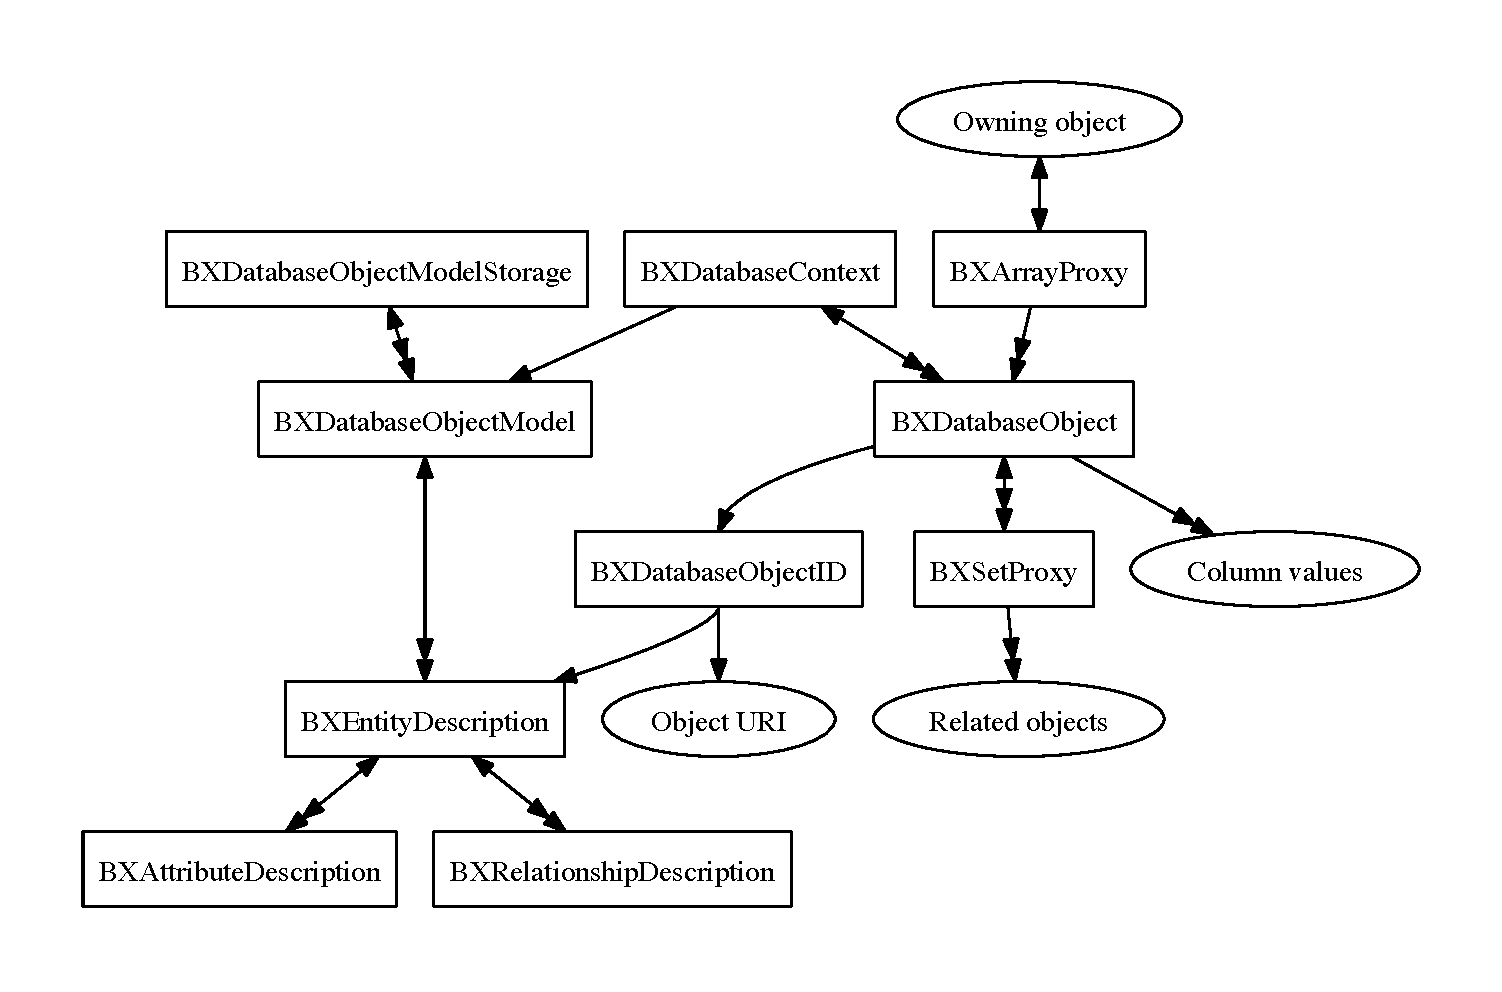
\includegraphics[width=\textwidth]{object-relationships}
\caption{Relationships between Base\+Ten's objects}
\end{DoxyImage}
 
\begin{DoxyImage}
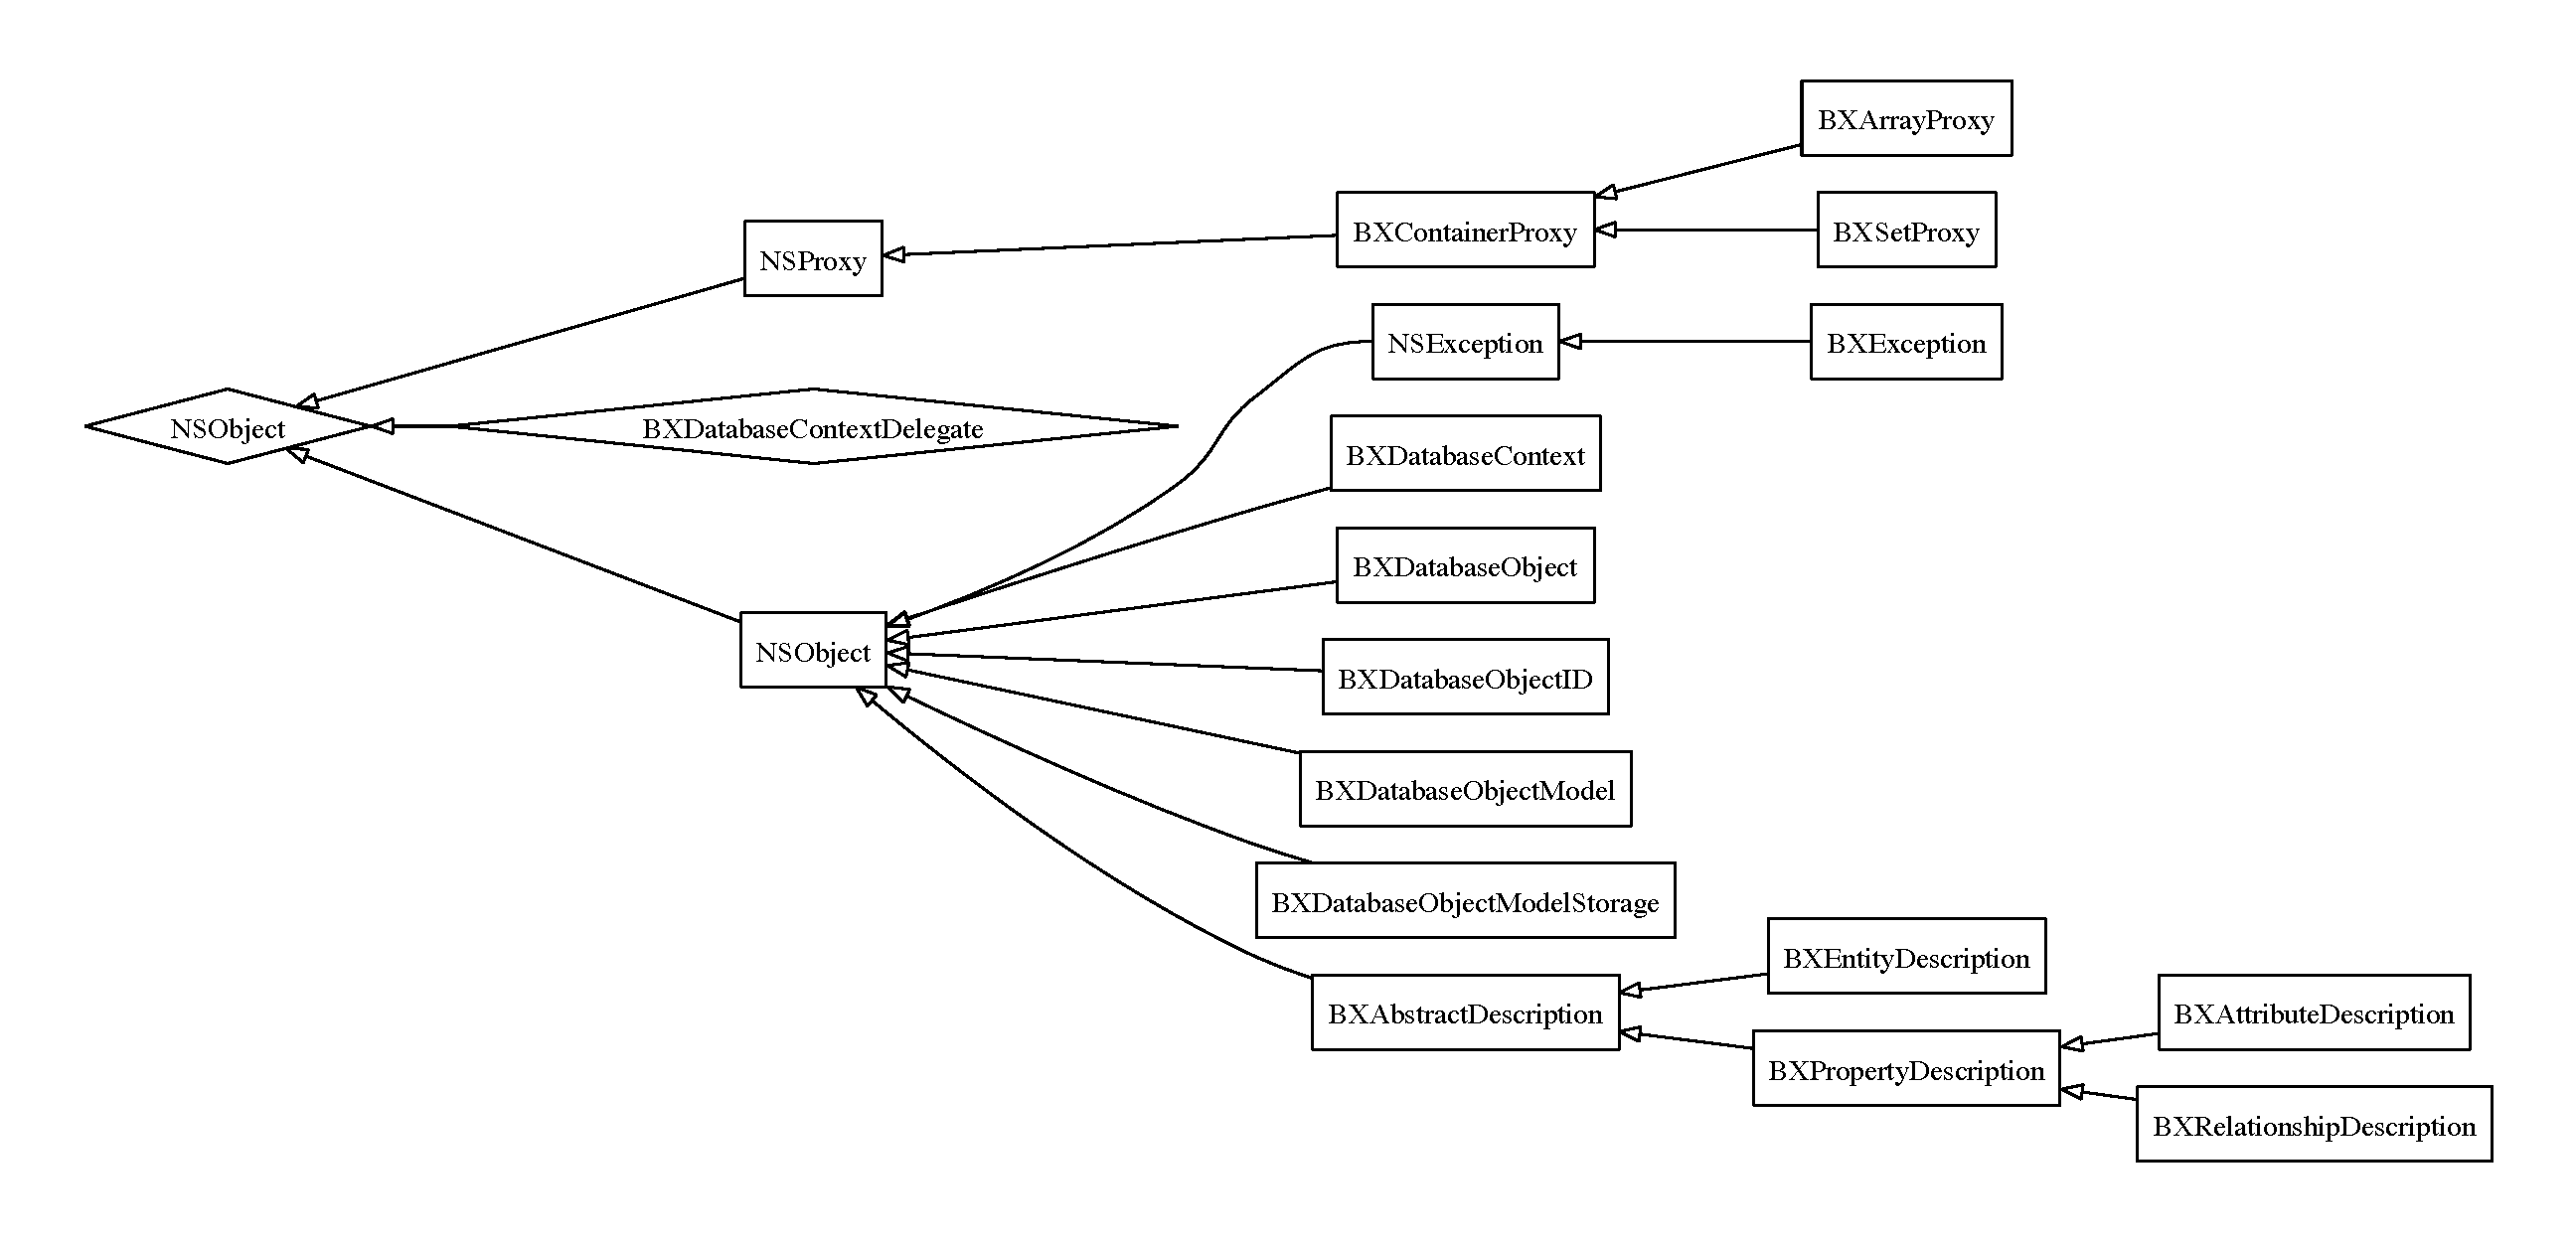
\includegraphics[width=\textwidth]{class-hierarchy}
\caption{Base\+Ten class hierarchy}
\end{DoxyImage}
 \hypertarget{baseten_assistant}{}\section{Base\+Ten Assistant}\label{baseten_assistant}
Base\+Ten Assistant is a simple database management application distributed with Base\+Ten framework. It has its own help that is available from within the application. In short, it has the following features\+: \begin{DoxyItemize}
\item It can be used to enable or disable tables and views for use with Base\+Ten. \item It can refresh the tables that Base\+Ten uses to determine relationships between entities. \item It can list entities' attributes and relationships as they are available when using the framework. \item It can create a database schema from an Xcode data model. \item It can create a chart of the database schema that can be displayed using Graphviz or Omni\+Graffle. \end{DoxyItemize}
\hypertarget{getting_started}{}\section{Getting started}\label{getting_started}
Typically accessing a database consists roughly of the following steps\+: 
\begin{DoxyItemize}
\item \hyperlink{getting_started_creating_a_database_context}{Creating an instance of B\+X\+Database\+Context} 
\item \hyperlink{getting_started_connecting_to_a_database}{Connecting to a database} 
\item \hyperlink{getting_started_getting_an_entity_and_a_predicate}{Getting an entity description from the context and possibly creating an N\+S\+Predicate for reducing the number of fetched objects} 
\item \hyperlink{getting_started_performing_a_fetch}{Performing a fetch using the entity and the predicate} 
\item \hyperlink{getting_started_handling_the_results}{Handling the results} 
\item \hyperlink{getting_started_creating_objects}{Creating new objects} 
\end{DoxyItemize}Here is a small walkthrough with sample code. More examples are available in the Base\+Ten Subversion repository and at \href{http://basetenframework.org}{\tt http\+://basetenframework.\+org}.

 
  \lstset{language=[Objective]C, backgroundcolor=\color[rgb]{0.84,0.87,0.90}, rulecolor=\color[gray]{0.53}, frame=single, framesep=0pt, framextopmargin=2pt, framexbottommargin=2pt, fontadjust, columns=fullflexible, captionpos=b}
  \begin{lstlisting}[caption=A simple command line tool that uses BaseTen]
  #import <Foundation/Foundation.h>
  #import <BaseTen/BaseTen.h>
 
  int main (int argc, char** argv)
  {
      NSURL* databaseURI = [NSURL URLWithString: @"pgsql://username@localhost/database"];
      BXDatabaseContext* ctx = [[BXDatabaseContext alloc] initWithDatabaseURI: databaseURI];
  
      [ctx connectSync: NULL];
      BXEntityDescription* entity = [[ctx databaseObjectModel] entityForTable: @"table"];
      NSArray* result = [ctx executeFetchForEntity: entity withPredicate: nil error: NULL];
 
      for (BXDatabaseObject* object in result)
      {
          NSLog (@"Object ID: %@ column: %@", 
                 [[object objectID] URIRepresentation], [object valueForKey: @"column"]);
      }
 
      NSDictionary* values = [NSDictionary dictionaryWithObject: @"newValue" forKey: @"column"];
      BXDatabaseObject* newObject = [ctx createObjectForEntity: entity 
                                      withFieldValues: values error: NULL];
      NSLog (@"new object: %@", newObject);
 
      return 0;
  }
  \end{lstlisting} 
   \hypertarget{getting_started_creating_a_database_context}{}\subsection{Creating a database context}\label{getting_started_creating_a_database_context}
The designated initializer of B\+X\+Database\+Context is -\/init\+With\+Database\+U\+R\+I\+:. -\/init is also available but the context does require an U\+R\+I before connecting.

B\+X\+Database\+Context requires the U\+R\+I to be formatted as follows\+:~\newline
 {\ttfamily pgsql\+://username\+:password@host/database\+\_\+name}. Currently, as Postgre\+S\+Q\+L is the only supported database, only {\ttfamily pgsql\+://} U\+R\+Is are allowed. In command line tools, all parameters are required except for the password, the need for which depends on the database configuration.

Various methods in B\+X\+Database\+Context take a double pointer to an N\+S\+Error object as a parameter. if the called method fails, the N\+S\+Error will be set on return. If the parameter is N\+U\+L\+L, the default error handler raises a \hyperlink{interface_b_x_exception}{B\+X\+Exception}. B\+X\+Database\+Context's delegate may change this behaviour.\hypertarget{getting_started_connecting_to_a_database}{}\subsection{Connecting to a database}\label{getting_started_connecting_to_a_database}
 
  \begin{lstlisting}
  [ctx connectSync: NULL];
  \end{lstlisting}
   

Connection to the database may be made synchronously using the method -\/connect\+Sync. Applications that use an N\+S\+Run\+Loop also have the option to use -\/connect\+Async. The method returns immediately. When the connection attempt has finished, the context's delegate will be called and notifications will be posted to the context's notification center (accessed with -\/notification\+Center).

In App\+Kit applications, the easiest way to connect to the database is to use the I\+B\+Action -\/connect\+:. In addition to attempting the connection asynchronously, it also presents a number of panels to the user, if some required information is missing from the U\+R\+I. The panels allow the user to specify their username, password and the database host making U\+R\+Is like {\ttfamily pgsql\+:///{\itshape database\+\_\+name}} allowed. Additionally a {\itshape k\+B\+X\+Connection\+Setup\+Alert\+Did\+End\+Notification} will be posted when the user dismisses an alert panel, which is presented on failure.

Since {\itshape N\+U\+L\+L} is passed in place of an N\+S\+Error double pointer, a \hyperlink{interface_b_x_exception}{B\+X\+Exception} will be thrown on error. See B\+X\+Database\+Context's documentation for details on error handling.\hypertarget{getting_started_getting_an_entity_and_a_predicate}{}\subsection{Getting a B\+X\+Entity\+Description and an N\+S\+Predicate}\label{getting_started_getting_an_entity_and_a_predicate}
 
  \begin{lstlisting}
  BXEntityDescription* entity = [[ctx databaseObjectModel] entityForTable: @"table"];
  \end{lstlisting}
   

B\+X\+Entity\+Descriptions are used to specify tables for fetches. For getting a specific entity description, \hyperlink{interface_b_x_database_object_model}{B\+X\+Database\+Object\+Model} has two methods\+: -\/entity\+For\+Table\+: and -\/entity\+For\+Table\+:in\+Schema\+:. Entity descriptions may be accessed before making a connection in which case the database context will check their existence on connect.

N\+S\+Predicates are created by various Cocoa objects and may be passed directly to B\+X\+Database\+Context. One way to create ad-\/hoc predicates is by using N\+S\+Predicate's method -\/predicate\+With\+Format\+:. In this example, we fetch all the objects instead of filtering them, though.\hypertarget{getting_started_performing_a_fetch}{}\subsection{Performing a fetch using the entity and the predicate}\label{getting_started_performing_a_fetch}
 
  \begin{lstlisting}
  NSArray* result = [ctx executeFetchForEntity: entity withPredicate: nil error: NULL];
  \end{lstlisting}
   

B\+X\+Database\+Context's method -\/execute\+Fetch\+For\+Entity\+:with\+Predicate\+:error\+: and its variations may be used to fetch objects from the database. The method takes a \hyperlink{interface_b_x_entity_description}{B\+X\+Entity\+Description} and an N\+S\+Predicate and performs a fetch synchronously. The fetched objects are returned in an N\+S\+Array.\hypertarget{getting_started_handling_the_results}{}\subsection{Handling the results}\label{getting_started_handling_the_results}
 
  \begin{lstlisting}
  for (BXDatabaseObject* object in result)
  {
     NSLog (@"Object ID: %@ column: %@", 
            [[object objectID] URIRepresentation], [object valueForKey: @"column"]);
  } 
  \end{lstlisting}
   

Since \hyperlink{interface_b_x_database_object}{B\+X\+Database\+Object} conforms to {\itshape N\+S\+Key\+Value\+Observing}, methods -\/value\+For\+Key\+: and -\/set\+Value\+:for\+Key\+: are available. See \hyperlink{accessing_values}{Accessing object values} for details.\hypertarget{getting_started_creating_objects}{}\subsection{Creating a new object}\label{getting_started_creating_objects}
 
  \begin{lstlisting}
  NSDictionary* values = [NSDictionary dictionaryWithObject: @"newValue" forKey: @"column"];
  BXDatabaseObject* newObject = [ctx createObjectForEntity: entity 
                                  withFieldValues: values error: NULL];
  NSLog (@"new object: %@", newObject);
  \end{lstlisting}
   

New rows are inserted with B\+X\+Database\+Context's method -\/create\+Object\+For\+Entity\+:with\+Field\+Values\+:error\+:. The values dictionary may contain initial values for both attributes and to-\/one relationships in case the target entity contains the foreign key. \hypertarget{accessing_values}{}\section{Accessing object values}\label{accessing_values}
B\+X\+Database\+Objects implement N\+S\+Key\+Value\+Coding and object values may thus be accessed with -\/value\+For\+Key\+: and -\/set\+Value\+:for\+Key\+:. The key will be the column name. As with N\+S\+Managed\+Object, methods like -\/{\itshape key} and -\/set{\itshape Key}\+: are also automatically available.

Column values are converted to Foundation objects based on the column type. Currently, there is no way to affect the type conversion. Instead, custom getters may be written for preprocessing fetched objects. To support this, the column values may also be accessed using \hyperlink{interface_b_x_database_object_a0576661b8930420dce5248584dfc1add}{-\/primitive\+Value\+For\+Key\+:}. Similarly -\/set\+Primitive\+Value\+:for\+Key\+: may be used to set a column value.

Currently handled data types are listed in \hyperlink{database_types}{Handled Postgre\+S\+Q\+L types}.

 
\begin{sidewaysfigure}
 
\begin{DoxyImage}
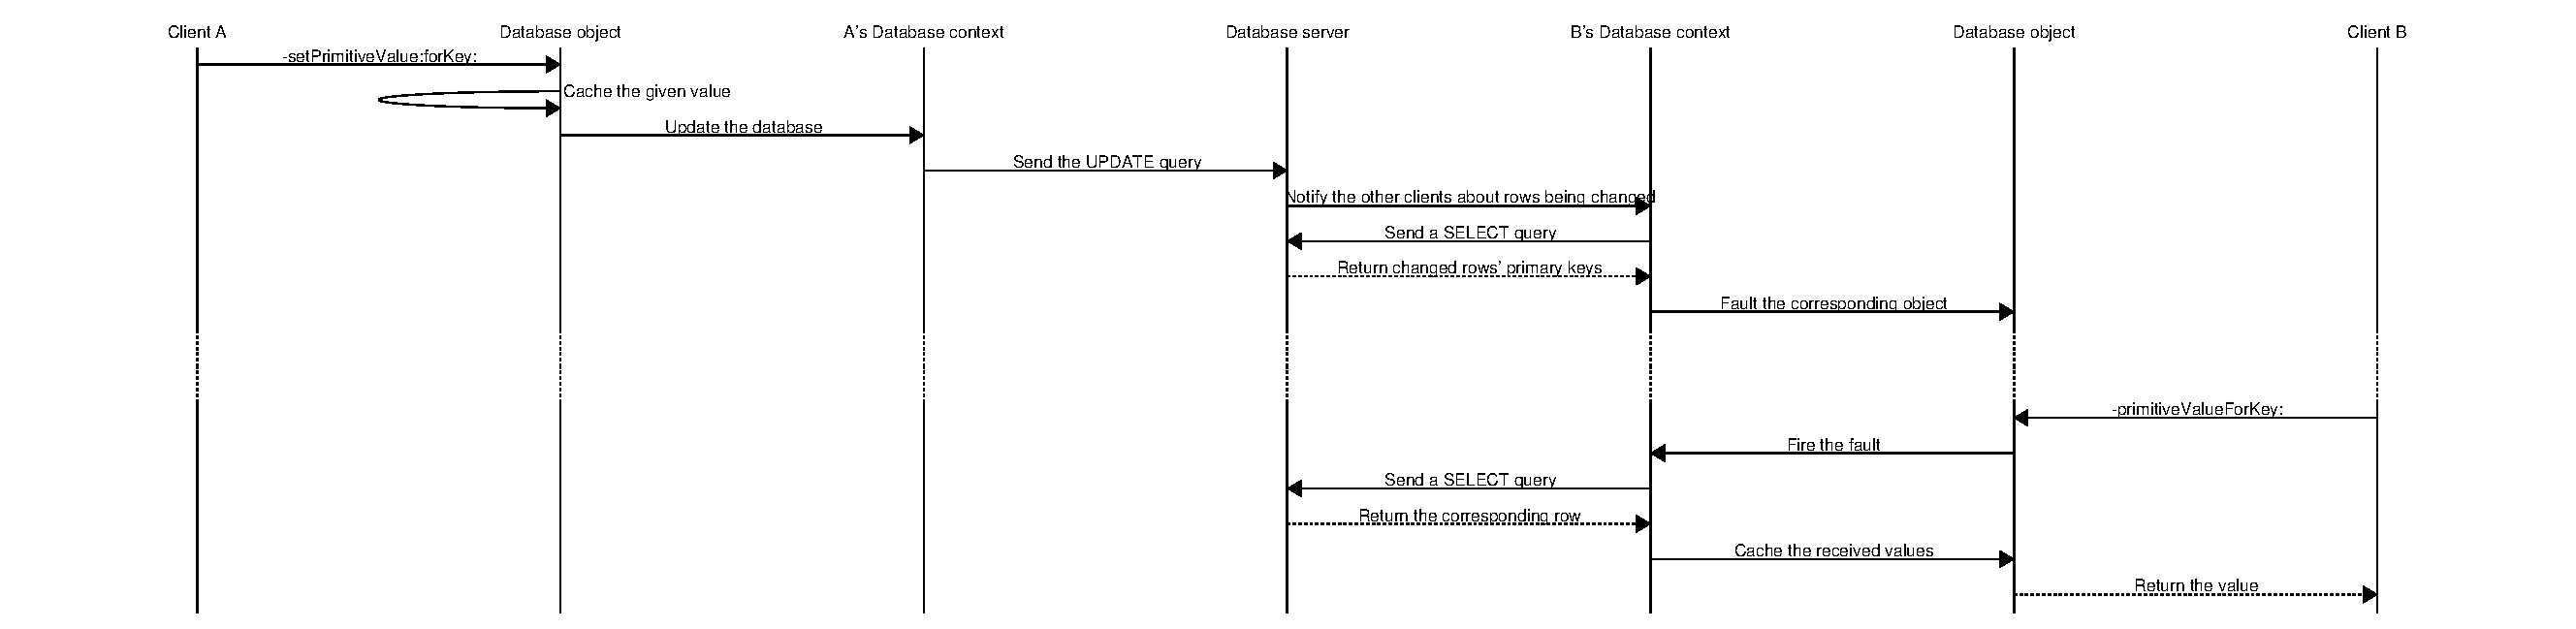
\includegraphics[width=\textheight]{update-change-propagation}
\caption{Objects being accessed by other clients are automatically faulted as part of the update process.}
\end{DoxyImage}
  
\end{sidewaysfigure}
 \hypertarget{sql_views}{}\section{S\+Q\+L views}\label{sql_views}
Contents of S\+Q\+L views may be manipulated using database objects provided that some conditions are met. Unlike tables, views don't have primary keys but Base\+Ten still needs to be able to reference individual rows. If a view has a group of columns that can act as a primary key, the columns may be marked as a primary key with the assistant, after which the view may be enabled.

Views also lack foreign keys. Despite this entities that correspond to views may have relationships provided that a certain condition is met\+: the view needs to have the column or columns of an underlying table that form a foreign key, and the columns' names need to match. In this case, relationships will be created between the view and the target table as well as the view and all the views that are based on the target table and contain the columns the foreign key references to. This applies to the complete view hierarchy.

Postgre\+S\+Q\+L allows I\+N\+S\+E\+R\+T and U\+P\+D\+A\+T\+E queries to target views if rules have been created to handle them. In this case, the view contents may be modified also with Base\+Ten. \hypertarget{database_types}{}\section{Handled Postgre\+S\+Q\+L types}\label{database_types}
Composite types, domains and types not listed here are currently returned as N\+S\+Data. Array types are returned as N\+S\+Arrays of the respective type or N\+S\+Arrays of N\+S\+Data objects.

\begin{table}[h]\begin{TabularC}{2}
\hline
\rowcolor{lightgray}{\bf {\bfseries Postgre\+S\+Q\+L type} }&{\bf {\bfseries Cocoa type}  }\\\cline{1-2}
aclitem &(A private class)  \\\cline{1-2}
bigint, bigserial &N\+S\+Number  \\\cline{1-2}
bit &N\+S\+String  \\\cline{1-2}
boolean &N\+S\+Number  \\\cline{1-2}
bytea &N\+S\+Data  \\\cline{1-2}
char, bpchar &N\+S\+String  \\\cline{1-2}
date &N\+S\+Date  \\\cline{1-2}
decimal, numeric &N\+S\+Decimal\+Number  \\\cline{1-2}
double precision &N\+S\+Number  \\\cline{1-2}
int2vector &N\+S\+Array of N\+S\+Numbers  \\\cline{1-2}
integer, serial &N\+S\+Number  \\\cline{1-2}
name &N\+S\+String  \\\cline{1-2}
oid &N\+S\+Number  \\\cline{1-2}
point &N\+S\+Value  \\\cline{1-2}
real &N\+S\+Number  \\\cline{1-2}
smallint &N\+S\+Number  \\\cline{1-2}
text &N\+S\+String  \\\cline{1-2}
time &N\+S\+Date  \\\cline{1-2}
time with time zone &N\+S\+Date  \\\cline{1-2}
timestamp &N\+S\+Date  \\\cline{1-2}
timestamp with time zone &N\+S\+Date  \\\cline{1-2}
varbit &N\+S\+String  \\\cline{1-2}
varchar &N\+S\+String  \\\cline{1-2}
uuid &N\+S\+String  \\\cline{1-2}
xml &N\+S\+Data or N\+S\+X\+M\+L\+Document  \\\cline{1-2}
\end{TabularNC}
\centering
\caption{Type conversion}
\end{table}
\hypertarget{database_types_string_handling}{}\subsection{String types}\label{database_types_string_handling}
When N\+S\+Strings are passed to the database, they are normalized to Unicode N\+F\+D. In case the database's encoding isn't Unicode (U\+T\+F-\/8), Postgre\+S\+Q\+L will handle the conversion.

Even if the database's encoding is Unicode, Postgre\+S\+Q\+L compares bytes, not Unicode characters, in strings as of version 8.\+3. Thus, comparison within the database could fail when done with non-\/normalized strings or strings in N\+F\+C.\hypertarget{database_types_date_handling}{}\subsection{Date and time types}\label{database_types_date_handling}
Cocoa's and Core Foundation's date classes store the date as seconds from a reference date, 2001-\/01-\/01 00\+:00\+:00 U\+T\+C. S\+Q\+L times and timestamps, on the other hand, might have an associated time zone specified as an offset to G\+M\+T. In Postgre\+S\+Q\+L 8.\+3, removing the time zone information by casting truncates the value. Casting a time or a timestamp lacking a time zone assigns the current time zone to it instead of converting.

Base\+Ten does several things to cope with this\+: \begin{DoxyItemize}
\item It sets the connection's time zone to U\+T\+C. \item It assigns U\+T\+C to times and timestamps that don't have a time zone. \item It converts received times and timestamps in other time zones to U\+T\+C. \item N\+S\+Calendar\+Dates passed as parameters will be converted to U\+T\+C.\end{DoxyItemize}
Therefore, N\+S\+Dates received from the server should in fact contain the offset from their point in time to the reference date. To ease handling, the date is set to 2001-\/01-\/01 in case of time types. This allows -\/\mbox{[}N\+S\+Date time\+Interval\+Since\+Reference\+Date\mbox{]} to return the time's difference to midnight in seconds.

N\+S\+Dates are converted to their date representation using N\+S\+Calendar and its underlying I\+C\+U library. I\+C\+U specifies a single cut-\/over date for the switch from Julian to Gregorian calendar, which is 1582-\/10-\/04. (It isn't currently possible to specify a different cut-\/over date to N\+S\+Calendar.) N\+S\+Dates before this point will be converted to Julian calendar dates. The rationale for this is that timestamps can't be passed directly to Postgre\+S\+Q\+L, and N\+S\+Calendar seems to be the best option for representing timestamps as dates. Postgre\+S\+Q\+L, on the other hand, uses Julian days (number of days since January 1, 4713 B\+C\+E with fraction, length of the year specified as 365.\+2425 days) for date calculations, and most likely converts them to Gregorian calendar dates for presentation. Thus, your mileage may vary when calculating dates within the database.

\begin{DoxyNote}{Note}
In versions earlier than 1.\+7, date handling depended on several factors, such as the current time zone and the server's time zone. This is no longer the case. Also, all date and time types are currently returned as N\+S\+Date, not N\+S\+Calendar\+Date.
\end{DoxyNote}
\hypertarget{database_types_xml_handling}{}\subsection{The X\+M\+L type}\label{database_types_xml_handling}
Postgre\+S\+Q\+L's xml data type handles both X\+M\+L documents and content fragments. Base\+Ten creates N\+S\+Data objects from them by default, but if the table also has a constraint like {\itshape C\+H\+E\+C\+K (xml\+\_\+column I\+S D\+O\+C\+U\+M\+E\+N\+T)}, N\+S\+X\+M\+L\+Documents will be created instead. The constraint mustn't contain any other conditions, but there may be additional C\+H\+E\+C\+K constraints.\hypertarget{database_types_custom_database_types}{}\subsection{Requirements for custom base data types}\label{database_types_custom_database_types}
In case of Base\+Ten-\/enabled tables, column contents are compared on update to determine, which columns did actually change. Thus, any custom base data types (created with {\itshape C\+R\+E\+A\+T\+E T\+Y\+P\+E}) used in these tables need to have the equality operator {\itshape =}. Currently, the operator needs to be accessible using the default search path. In case the custom type is such that the concept of equality doesn't apply, the operator may always return {\itshape false}. In this case the value for the column will always be fetched when the corresponding row changes.

Base\+Ten provides custom equality operators for Postgre\+S\+Q\+L's geometric types, for which the default equality operator would only compare equal areas. \hypertarget{relationships}{}\section{Relationships}\label{relationships}
Base\+Ten supports the same types of relationships as Core Data\+: one-\/to-\/one, one-\/to-\/many and many-\/to-\/many. After Base\+Ten schema has been installed, relationships are created using foreign keys as shown in the following table.

\begin{table}[h]\begin{TabularC}{2}
\hline
\rowcolor{lightgray}{\bf {\bfseries Relationship type} }&{\bf {\bfseries Required conditions}  }\\\cline{1-2}
One-\/to-\/many &A foreign key constraint on the many-\/side.  \\\cline{1-2}
One-\/to-\/one &A foreign key constraint the columns of which also have an unique constraint.  \\\cline{1-2}
Many-\/to-\/many &A helper table that has foreign keys referencing two other tables. The foreign key columns also need to form the table's primary key.  \\\cline{1-2}
\end{TabularNC}
\centering
\caption{Required conditions for relationsips}
\end{table}


\begin{DoxyNote}{Note}
Before Base\+Ten 1.\+8, relationships were only available in enabled tables and views.
\end{DoxyNote}
\hypertarget{relationships_relationship_naming}{}\subsection{Relationship naming}\label{relationships_relationship_naming}
Relationship names are determined from foreign key names. For one-\/to-\/one and one-\/to-\/many relationships, the foreign key's name should have the form {\itshape name1\+\_\+\+\_\+name2}, where {\itshape name1} is the relationship's name from the foreign key's side, and {\itshape name2} is the inverse relationship's name. If the foreign key's name doesn't contain two consecutive underscores, a generated name is used for the inverse relationship. Similarly, if the foreign key's name begins with two underscores, a generated name is used for the relationship. The generated name has the format {\itshape schema\+\_\+table\+\_\+foreignkey}.

Many-\/to-\/many relationships have the same name as the foreign key that references the target table.

Base\+Ten Assistant generates foreign keys with names like this, but if creating or altering the database schema isn't an option, a set of identical relationships is created with different names. Each relationship has the same name as the target table, with the word “\+Set” appended in the case of to-\/many relationships.

The latter naming is also available with views, while the former is not.

In case the two relationships created into the same entity have matching names, the one named after the table and its inverse relationship are removed. In case two relationships created into one entity using different foreign keys have matching names, they will both be removed with their inverse relationships.

\begin{table}[h]\begin{TabularC}{2}
\hline
\rowcolor{lightgray}{\bf {\bfseries Relationship type} }&{\bf {\bfseries Available names}  }\\\cline{1-2}
One-\/to-\/many (inverse, from the foreign key's side) &{\itshape target}Set, first part of the foreign key's name  \\\cline{1-2}
One-\/to-\/many (from the referenced side) &{\itshape target}, second part of the foreign key's name  \\\cline{1-2}
One-\/to-\/one (from the foreign key's side) &{\itshape target}, first part of the foreign key's name  \\\cline{1-2}
One-\/to-\/one (from the referenced side) &{\itshape target}, second part of the foreign key's name  \\\cline{1-2}
Many-\/to-\/many &{\itshape target}Set, name of the foreign key that references the target table  \\\cline{1-2}
\end{TabularNC}
\centering
\caption{Relationship names}
\end{table}


\begin{DoxyNote}{Note}
The relationship names used before version 1.\+7 are still available. They won't be listed by Base\+Ten Assistant, though, and using them will call \hyperlink{_b_x_logger_8h_aebc9da21ce1d8bd8e13dee02d91e1e7d}{B\+X\+Deprecation\+Warning}.
\end{DoxyNote}
\hypertarget{relationships_relationship_naming_example}{}\subsection{Relationship example}\label{relationships_relationship_naming_example}
Consider the following case\+:  
  \lstset{language=SQL, backgroundcolor=\color[rgb]{0.84,0.87,0.90}, rulecolor=\color[gray]{0.53}, frame=single, framesep=0pt, framextopmargin=2pt, framexbottommargin=2pt, fontadjust, columns=fullflexible, captionpos=b}
  \begin{lstlisting}[caption=Tables with a one-to-many relationship]
  CREATE TABLE person (
      id SERIAL PRIMARY KEY,
      firstname VARCHAR (255),
      surname VARCHAR (255)
  );
 
  CREATE TABLE email (
      id SERIAL PRIMARY KEY,
      address VARCHAR (255),
      person_id INTEGER REFERENCES person (id)
  );
  \end{lstlisting} 
   

Lets say we have two objects\+: {\itshape a\+Person} and {\itshape an\+Email} which have been fetched from the person and email tables, respectively.~\newline
 {\ttfamily \mbox{[}a\+Person value\+For\+Key\+:@\char`\"{}email\+Set\char`\"{}\mbox{]}} will now return a collection of {\itshape email} objects.~\newline
 {\ttfamily \mbox{[}an\+Email value\+For\+Key\+:@\char`\"{}person\char`\"{}\mbox{]}} will return a single {\itshape person} object.

If we modify the previous example by adding an unique constraint, we get a one-\/to-\/one relationship\+:

 
  \begin{lstlisting}
  ALTER TABLE email ADD UNIQUE (person_id);
  \end{lstlisting} 
   

Now both of the following messages will return a single object from the corresponding table\+:~\newline
 {\ttfamily \mbox{[}a\+Person value\+For\+Key\+:@\char`\"{}email\char`\"{}\mbox{]}}~\newline
 {\ttfamily \mbox{[}an\+Email value\+For\+Key\+:@\char`\"{}person\char`\"{}\mbox{]}}

Many-\/to-\/many relationships are modeled with helper tables. The helper table needs to have columns to contain both tables' primary keys.

Another example\+:  
  \begin{lstlisting}[caption=Tables with a many-to-many relationship]
  CREATE TABLE person (
      id SERIAL PRIMARY KEY,
      firstname VARCHAR (255),
      surname VARCHAR (255)
  );
 
  CREATE TABLE title (
      id SERIAL PRIMARY KEY,
      name VARCHAR (255)
  );
 
  CREATE TABLE person_title_rel (
      person_id INTEGER REFERENCES person (id),
      title_id INTEGER REFERENCES title (id),
      PRIMARY KEY (person_id, title_id)
  );
  \end{lstlisting} 
   

Lets say {\itshape a\+Person} has been fetched from the person table and {\itshape a\+Title} from the title table. In this case,~\newline
 {\ttfamily \mbox{[}a\+Person value\+For\+Key\+:@\char`\"{}title\+Set\char`\"{}\mbox{]}} will return a collection of title objects and ~\newline
 {\ttfamily \mbox{[}a\+Title value\+For\+Key\+:@\char`\"{}person\+Set\char`\"{}\mbox{]}} a collection of person objects.~\newline
 Any two foreign keys in one table will be interpreted as a many-\/to-\/many relationship, if they also form the table's primary key. Objects from the helper table may be retrieved as with one-\/to-\/many relationships\+:~\newline
 {\ttfamily \mbox{[}a\+Person value\+For\+Key\+:@\char`\"{}person\+\_\+title\+\_\+rel\+Set\char`\"{}\mbox{]}}. \hypertarget{predicates}{}\section{Predicates}\label{predicates}
Cocoa predicates are used to fetch objects that match certain criteria. Key paths in predicates correspond to entity attributes and relationships.

Most types of predicates and expressions are converted to S\+Q\+L and sent to the database server. Others cause the returned object set to be filtered again on the client side. Specifically, the following use cases work in this manner\+: The affected part of the predicate is replaced with {\itshape true} (or {\itshape false}, if the part is inside an odd number of N\+O\+T predicates), and excess objects are removed from the result set after it has been received.


\begin{DoxyItemize}
\item Use of N\+S\+Custom\+Selector\+Predicate\+Operator\+Type 
\item A modifier other than N\+S\+Direct\+Predicate\+Modifier in combination with any of the following\+: 
\begin{DoxyItemize}
\item N\+S\+Begins\+With\+Predicate\+Operator\+Type 
\item N\+S\+Ends\+With\+Predicate\+Operator\+Type 
\item N\+S\+Matches\+Predicate\+Operator\+Type 
\item N\+S\+Like\+Predicate\+Operator\+Type 
\item N\+S\+Contains\+Predicate\+Operator\+Type 
\item N\+S\+In\+Predicate\+Operator\+Type 
\end{DoxyItemize}
\item Use of any of the following predicate options\+: 
\begin{DoxyItemize}
\item N\+S\+Diacritic\+Insensitive\+Predicate\+Option 
\item N\+S\+Normalized\+Predicate\+Option 
\item N\+S\+Locale\+Sensitive\+Predicate\+Option 
\end{DoxyItemize}
\item Use of any of the following expression types\+: 
\begin{DoxyItemize}
\item N\+S\+Subquery\+Expression\+Type 
\item N\+S\+Union\+Set\+Expression\+Type 
\item N\+S\+Intersect\+Set\+Expression\+Type 
\item N\+S\+Minus\+Set\+Expression\+Type 
\item N\+S\+Block\+Expression\+Type 
\end{DoxyItemize}
\item Use of a function expression with a custom target and selector 
\item Use of a function expression with any of the following predefined selectors\+: 
\begin{DoxyItemize}
\item average\+: 
\item cast\+Object\+:to\+Type\+: 
\item max\+: 
\item median\+: 
\item min\+: 
\item mode\+: 
\item random 
\item random\+: 
\item randomn\+: 
\item stddev\+: 
\end{DoxyItemize}
\end{DoxyItemize}\hypertarget{tracking_changes}{}\section{Tracking database changes}\label{tracking_changes}
\hyperlink{interface_b_x_database_object}{B\+X\+Database\+Object} conforms to N\+S\+Key\+Value\+Observing and uses self-\/updating collections for storing related objects; changes in them may thus be tracked with K\+V\+O.

\hyperlink{interface_b_x_synchronized_array_controller}{B\+X\+Synchronized\+Array\+Controller}'s contents will be updated automatically. B\+X\+Database\+Context's fetch methods also have the option to return a self-\/updating array instead of an ordinary one. In this case, the collection's owner has to be specified for K\+V\+O notifications to be posted. See the collection classes' documentation for details.

Another, a more low-\/level means of tracking changes is observing N\+S\+Notifications. Notifications on entity changes will be posted to the relevant context's notification center. The notification object will be a \hyperlink{interface_b_x_entity_description}{B\+X\+Entity\+Description} which corresponds to the table where the change happened. The names of the notifications are\+: \begin{DoxyItemize}
\item {\itshape k\+B\+X\+Insert\+Notification} on database {\itshape I\+N\+S\+E\+R\+T} \item {\itshape k\+B\+X\+Update\+Notification} on database {\itshape U\+P\+D\+A\+T\+E} \item {\itshape k\+B\+X\+Delete\+Notification} on database {\itshape D\+E\+L\+E\+T\+E}\end{DoxyItemize}
At the time the notifications are posted, database objects and self-\/updating collections will already have been updated.\hypertarget{tracking_changes_trigger_effects}{}\subsection{Effects of triggers}\label{tracking_changes_trigger_effects}
When inserting, updating or deleting rows, Base\+Ten notices (and posts notifications of) changes that occur as a result of database triggers or rules firing. The only requirement is that said changes are to entities other than the one being changed by Base\+Ten; changes to the same entity will be ignored. \hypertarget{using_appkit_classes}{}\section{Using Base\+Ten\+App\+Kit}\label{using_appkit_classes}
When Base\+Ten\+App\+Kit is linked to an application, B\+X\+Database\+Context gains some additional capabilities. If given a partial database U\+R\+I, it will present a number of connection panels when -\/connect\+: is called.

B\+X\+Database\+Objects may be used much in the same manner as N\+S\+Managed\+Objects to populate various Cocoa views. To handle some situations unique to Base\+Ten, some N\+S\+Controller subclasses have been provided with the framework. For now, the only directly usable one is \hyperlink{interface_b_x_synchronized_array_controller}{B\+X\+Synchronized\+Array\+Controller}. Additionally, there is \hyperlink{protocol_b_x_controller-p}{B\+X\+Controller} and additions to N\+S\+Controller for creating controller subclasses.

Base\+Ten\+App\+Kit contains a plug-\/in for Interface Builder. The plug-\/in should get loaded automatically if the framework is added to a project.

\begin{DoxyNote}{Note}
Under some circumstances the outlets and actions won't show up when the plug-\/in has been loaded for the first time. If this happens, save and close your document and open it again. Also relaunching Interface Builder has solved the issue.
\end{DoxyNote}
\hypertarget{using_appkit_classes_bxsynchronizedarraycontroller}{}\subsection{B\+X\+Synchronized\+Array\+Controller}\label{using_appkit_classes_bxsynchronizedarraycontroller}
Compared to N\+S\+Array\+Controller, \hyperlink{interface_b_x_synchronized_array_controller}{B\+X\+Synchronized\+Array\+Controller} can do the following things\+: 
\begin{DoxyItemize}
\item It can present errors to the user when creating a new object fails. 
\item It can get a \hyperlink{interface_b_x_entity_description}{B\+X\+Entity\+Description} from its database context and fetch objects using it. N\+S\+Entity\+Descriptions cannot be used because they are Core\+Data-\/specific. 
\item It can lock the edited row in the database when an editing session begins. 
\item It can provide the selected objects' ids. 
\end{DoxyItemize}

\hyperlink{interface_b_x_synchronized_array_controller}{B\+X\+Synchronized\+Array\+Controller} shouldn't be set to entity mode; the user interface for this isn't even available in Interface Builder. It also doesn't make use of a managed object context.

\hyperlink{interface_b_x_synchronized_array_controller}{B\+X\+Synchronized\+Array\+Controller}'s Content Set may be bound to another synchronized array controller with a key path that represents a relationship. In case of a one-\/to-\/many relationship, the foreign key field values will also be set when -\/new\+Object or -\/create\+Object\+: gets called.\hypertarget{using_appkit_classes_using_bxdatabasecontext_ib}{}\subsection{Using B\+X\+Database\+Context from Interface Builder}\label{using_appkit_classes_using_bxdatabasecontext_ib}

\begin{DoxyEnumerate}
\item Load the Base\+Ten plug-\/in. 
\item Create a new nib file. 
\item Drag a database context from the library to the file. 
\item Select the database context and choose Attributes from the inspector's pop-\/up menu. 
\item Enter a valid database U\+R\+I, {\ttfamily pgsql\+:///{\itshape database\+\_\+name}} at minimum. 
\end{DoxyEnumerate}\hypertarget{using_appkit_classes_using_bxsynchronizedarraycontroller_ib}{}\subsection{Using B\+X\+Synchronized\+Array\+Controller from Interface Builder}\label{using_appkit_classes_using_bxsynchronizedarraycontroller_ib}

\begin{DoxyEnumerate}
\item Drag a \hyperlink{interface_b_x_synchronized_array_controller}{B\+X\+Synchronized\+Array\+Controller} from the library to the file. 
\item Select the array controller and choose Attributes from the inspector's pop-\/up menu. 
\item Enter a table name into the field. 
\begin{DoxyItemize}
\item The schema field may be left empty, in which case {\itshape public} will be used. 
\end{DoxyItemize}
\item Bind the Cocoa views to the controller. 
\item Bind the array controller to the database context using the Database Context binding or connect the database\+Context outlet. 
\item Test the interface. The views should be populated using the database. 
\end{DoxyEnumerate}\hypertarget{using_appkit_classes_using_value_transformers_ib}{}\subsection{Using Base\+Ten\+App\+Kit's value transformers from Interface Builder}\label{using_appkit_classes_using_value_transformers_ib}
When database rows get locked, it might be desirable to disable editing and indicate this visually in the user interface. Most App\+Kit's classes, have an Editable binding, and some, like N\+S\+Table\+Column, have bindings that affect the display of their value. Lets say a table column's {\itshape Value} is bound to a B\+X\+Array\+Controller using {\itshape my\+\_\+key} as the model key path. Base\+Ten\+App\+Kit could then be used to set the rows to be conditionally editable like this\+: 
\begin{DoxyEnumerate}
\item Select the table column inside its table view 
\item Open the Bindings Inspector 
\item Click the Editable binding 
\item Set the binding to the array controller and set the controller key to {\itshape arranged\+Objects}. 
\item Set the model key to {\itshape status\+Info.\+my\+\_\+key}. 
\item Set the value transformer to {\itshape \hyperlink{interface_b_x_object_status_to_editable_transformer}{B\+X\+Object\+Status\+To\+Editable\+Transformer}}. 
\end{DoxyEnumerate}The rows may also be coloured so that their status is visible\+: 
\begin{DoxyEnumerate}
\item Inspecting the same column as in the previous example, click the Text Color binding. 
\item Set the binding to the array controller and set the controller key to {\itshape arranged\+Objects}. 
\item Set the model key to {\itshape status\+Info.\+my\+\_\+key}. 
\item Set the value transformer to {\itshape \hyperlink{interface_b_x_object_status_to_color_transformer}{B\+X\+Object\+Status\+To\+Color\+Transformer}}. 
\end{DoxyEnumerate}\hypertarget{autocommit_manual_commit}{}\section{Commit modes and locking}\label{autocommit_manual_commit}
B\+X\+Database\+Context has two modes for handling transactions, which affect queries sent to the database and the way the context's undo manager is used. In both cases, the transaction isolation level is set to R\+E\+A\+D C\+O\+M\+M\+I\+T\+T\+E\+D meaning that changes committed by other connections will be received. The commit mode is set using -\/set\+Autocommits\+:. Generally, autocommit is well-\/suited for non-\/document-\/based applications. Manual commit is well-\/suited for document-\/based applications, provided that changes are committed frequently enough.\hypertarget{autocommit_manual_commit_autocommit}{}\subsection{Autocommit}\label{autocommit_manual_commit_autocommit}
When using autocommit, each query creates its own transaction and changes get propagated immediately to other clients. Undo works at the level of -\/\mbox{[}\hyperlink{interface_b_x_database_object}{B\+X\+Database\+Object} set\+Primitive\+Value\+:for\+Key\+:\mbox{]}. For each change an invocation of the method is added to the undo manager with the earlier value as a parameter.\hypertarget{autocommit_manual_commit_manual_commit}{}\subsection{Manual commit}\label{autocommit_manual_commit_manual_commit}
In manual commit mode, a savepoint is added after each change. Undo causes a R\+O\+L\+L\+B\+A\+C\+K T\+O S\+A\+V\+E\+P\+O\+I\+N\+T query to be sent. This causes not only the changes made by Base\+Ten to be reverted, but their possible side effects as well. For instance, if database triggers fire when a specific change is made, its effects will be reverted, too. When -\/commit\+: or -\/rollback is called, undo queue is emptied.

In case one client updates a row, Base\+Ten doesn't send the change to other clients immediately. Instead, it sends a notification indicating that the row is locked and changing it will cause the connection to block until the other client ends its transaction. \hyperlink{interface_b_x_database_object}{B\+X\+Database\+Object}'s method -\/is\+Locked\+For\+Key\+:, B\+X\+Database\+Object\+Status\+Info class and value transformers in Base\+Ten\+App\+Kit are useful for handling this situation. However, other than Base\+Ten clients don't cause the lock status to be set, and the connection could block.

The downside is that if -\/\mbox{[}B\+X\+Database\+Context commit\+:\mbox{]} or -\/\mbox{[}B\+X\+Database\+Context rollback\mbox{]} aren't called frequently enough, transactions could become very long, which is against their intended use. This causes server resources to be consumed.\hypertarget{autocommit_manual_commit_locking_rows}{}\subsection{Locking rows}\label{autocommit_manual_commit_locking_rows}
When a database connection sends U\+P\+D\+A\+T\+E and D\+E\+L\+E\+T\+E queries, the affected rows will be locked until the connection ends its transaction. If other connections try to change the rows, their queries will block. To handle this situation, Base\+Ten stores information about locked rows into its internal tables and notifies other Base\+Ten clients about them. \hyperlink{interface_b_x_synchronized_array_controller}{B\+X\+Synchronized\+Array\+Controller} also tries to lock rows when the editing session begins.

Lock information will be available using \hyperlink{interface_b_x_database_object}{B\+X\+Database\+Object}'s method -\/is\+Locked\+For\+Key\+:. B\+X\+Database\+Context has a method, -\/set\+Sends\+Lock\+Queries\+:, for enabling or disabling lock notifications. If the notifications are disabled, B\+X\+Database\+Context won't notify other clients but still reacts to received notifications.

When editing rows through \hyperlink{interface_b_x_synchronized_array_controller}{B\+X\+Synchronized\+Array\+Controller}, it tries to send a S\+E\+L\+E\+C\+T ... F\+O\+R U\+P\+D\+A\+T\+E N\+O\+W\+A\+I\+T query when the editing session begins. If the context is in autocommit mode, a transaction will also be started. If the query succeeds, a lock notification will be sent regardless of B\+X\+Database\+Context's setting. If the query fails, the editing session will be ended using -\/discard\+Editing. \hyperlink{interface_b_x_synchronized_array_controller}{B\+X\+Synchronized\+Array\+Controller}'s method -\/set\+Locks\+Rows\+On\+Begin\+Editing\+: can be used to disable this functionality.

To make the changes visible in the user interface, Base\+Ten\+App\+Kit has some N\+S\+Value\+Transformer subclasses. See \hyperlink{group__value__transformers}{Value Transformers} for details. \hypertarget{thread_safety}{}\section{Thread safety}\label{thread_safety}
For its mostly used parts, Base\+Ten isn't thread safe. In particular, B\+X\+Database\+Context needs to be used from the same thread in which its connection methods have been called. This is because it adds a run loop source to the thread's run loop.

The documented methods of the following classes are thread safe\+:

\begin{DoxyItemize}
\item \hyperlink{interface_b_x_entity_description}{B\+X\+Entity\+Description} \item \hyperlink{interface_b_x_attribute_description}{B\+X\+Attribute\+Description} \item \hyperlink{interface_b_x_relationship_description}{B\+X\+Relationship\+Description} \item \hyperlink{interface_b_x_database_object_i_d}{B\+X\+Database\+Object\+I\+D}\end{DoxyItemize}
Additionally, \hyperlink{interface_b_x_database_object}{B\+X\+Database\+Object}'s method -\/cached\+Value\+For\+Key\+: is thread safe. As a result, \hyperlink{interface_b_x_database_object}{B\+X\+Database\+Object}'s values may be accessed from multiple threads as soon as they have been fetched.

One possibility to make use of multiple threads is to create a database context for each thread, but see \hyperlink{multiple_contexts}{the next chapter}. \hypertarget{multiple_contexts}{}\section{Using multiple database contexts}\label{multiple_contexts}
In general, there aren't many reasons to have multiple database contexts in an application that connects to a single database. One possibility to make the context available everywhere it's needed is to make it a property of the N\+S\+Application delegate or an N\+S\+Document subclass.

Advantages\+: \begin{DoxyItemize}
\item Thread safety. Since database contexts should be created and used from within a single thread, it might be advantageous to create one for each thread. \item Transaction isolation. One could want to query the database state outside the current transaction. \item Privilege separation. One might want to access the database using roles with different privileges. \item Different commit modes.\end{DoxyItemize}
Disadvantages\+: \begin{DoxyItemize}
\item Increased memory usage on the server. Each database context makes a connection to the database (two in manual commit mode). These require an amount of shared memory on the server. This limits the number of clients who can connect simultaneously. \item Increased memory and network usage on the client side. Database objects are uniqued and updated within a context, so each context requires its own copy of the objects. Each context also needs to update its objects on its own. \item Database objects cannot be passed from one context to another. This causes problems. \end{DoxyItemize}
\hypertarget{linking_to_baseten}{}\section{Linking to Base\+Ten and Base\+Ten\+App\+Kit}\label{linking_to_baseten}
Mac O\+S X's linker specifies paths to dynamic libraries (including frameworks) using a the install name of the library. The install name is specified in the library itself. Base\+Ten and Base\+Ten\+App\+Kit distributed on the disk image have their install names set to a location inside the loading application's bundle, in the Frameworks folder. When linking to the frameworks in Xcode, a Copy Files build phase should be added for the application target\+: 
\begin{DoxyEnumerate}
\item Right-\/click your application target in the Groups \& Files table 
\item Select Add, New Build Phase and New Copy Files Build Phase 
\item Select Frameworks as the destination 
\item Click the disclosure triangle next to your target 
\item Drag Base\+Ten and Base\+Ten\+App\+Kit inside the new build phase 
\end{DoxyEnumerate}

The frameworks are built with the -\/headerpad\+\_\+max\+\_\+install\+\_\+names linker option, so changing the install names with tools like install\+\_\+name\+\_\+tool should also be possible. When building Base\+Ten and Base\+Ten\+App\+Kit using the Debug configuration, the install name is left empty, which causes it to be set to the build directory. \hypertarget{building_baseten}{}\section{Building Base\+Ten}\label{building_baseten}
For a successful build, Xcode 3.\+1 and Mac O\+S X 10.\+5 S\+D\+K are required.

Base\+Ten has several subprojects, namely Base\+Ten\+App\+Kit and a plug-\/in for Interface Builder 3. The default target in Base\+Ten.\+xcodeproj, {\itshape Base\+Ten + G\+C}, builds them as well; the plug-\/in and the App\+Kit framework will appear in the subprojects' build folders, which are set to the default folder. The built files will be either in {\itshape build} folders in the subprojects' folders or in the user-\/specified build folder. The documentation will be in the {\itshape Documentation} folder.\hypertarget{building_baseten_building_for_the_release_dmg}{}\subsection{Building for the release disk image}\label{building_baseten_building_for_the_release_dmg}
The files needed to build the release disk image are in the S\+V\+N repository as well. Doxygen is needed during the process. To create the D\+M\+G, follow these steps\+: 
\begin{DoxyEnumerate}
\item From the checked-\/out directory, {\ttfamily cd Release\+D\+M\+G}. 
\item The default location for the built files is {\itshape Base\+Ten-\/dmg-\/build} in the current directory. To set a custom path, edit the {\itshape S\+Y\+M\+R\+O\+O\+T} variable in {\itshape create\+\_\+release\+\_\+dmg.\+sh}. 
\item Do {\ttfamily ./create\+\_\+release\+\_\+dmg.sh}. The built D\+M\+G will appear in the {\itshape Release\+D\+M\+G} folder. 
\begin{DoxyItemize}
\item If you don't have La\+Te\+X installed, do {\ttfamily ./create\+\_\+release\+\_\+dmg.sh -\/--without-\/latex} instead. The P\+D\+F manual won't be included on the D\+M\+G, though. 
\end{DoxyItemize}
\end{DoxyEnumerate}
\chapter{Database administration}
\label{database_usage}
\hypertarget{database_usage}{}
 \section*{Topics}  \begin{DoxyItemize}
\item \hyperlink{baseten_enabling}{Enabling relations for use with Base\+Ten} \item \hyperlink{database_dumps}{Making a database dump} \item \hyperlink{postgresql_installation}{Postgre\+S\+Q\+L installation} \end{DoxyItemize}
\hypertarget{baseten_enabling}{}\section{Enabling relations for use with Base\+Ten}\label{baseten_enabling}
Some tables are created in Base\+Ten schema to track changes in other relations and storing relationships between tables and views. The association is based on relation names.

While this arrangement allows clients to fault only changed objects, it has some unfortunate side effects\+: \begin{DoxyItemize}
\item Altering relations' names after having them enabled will not work. To rename relations, they need to be disabled first and re-\/enabled afterwards. \item Altering relations' primary keys will not work. Again, disabling and re-\/enabling is required. \item Altering relations' columns will not work. Again, disabling and re-\/enabling is required. \item Altering relations' foreign keys causes Base\+Ten's relationship information to become out-\/of-\/date and needing to be refreshed.\end{DoxyItemize}
All this can be done using Base\+Ten Assistant.

\begin{DoxyNote}{Note}
In version 1.\+5, relations and Base\+Ten's tables were associated with each other based on relation names. This didn't work for all names, though, and made renaming enabled relations impossible. In versions 1.\+6 through 1.\+6.\+2, the association was based on relation oids. While this made renaming relations possible, it also made dumping database contents exceedingly difficult.
\end{DoxyNote}
\hypertarget{baseten_enabling_sql_enabling}{}\subsection{Enabling relations and updating relationship cache using S\+Q\+L functions}\label{baseten_enabling_sql_enabling}
In addition to using Base\+Ten Assistant, it is possible to enable and disable tables with S\+Q\+L functions. The functions are {\itshape baseten.\+enable (oid)} and {\itshape baseten.\+disable (oid)}. The object identifier argument can be looked up from Postgre\+S\+Q\+L's system tables, {\itshape pg\+\_\+class} and {\itshape pg\+\_\+namespace}.

Views' primary keys are stored in {\itshape baseten.\+view\+\_\+pkey}. The table has three columns\+: {\itshape nspname}, {\itshape relname} and {\itshape attname}, which correspond to the view's schema name, the view's name and each primary key column's name respectively. To enable a view, its primary key needs to be specified first.

Relationships and view hierarchies among other things are stored in automatically-\/generated tables. These should be refreshed with the S\+Q\+L function {\itshape baseten.\+refresh\+\_\+caches ()} after all changes to views, primary keys and foreign keys. \hypertarget{database_dumps}{}\section{Making a database dump}\label{database_dumps}
After having been in use, the Base\+Ten schema might contain some temporary information. The temporary information is removed periodically when the database is queried, but for creating installation scripts it might be desirable to remove all unnecessary data. This can be done from Base\+Ten Assistant or by running the S\+Q\+L function {\itshape baseten.\+prune ()}.

For Base\+Ten schema to work, the table contents for most tables are needed, so dumps excluding the data are not recommended. \hypertarget{postgresql_installation}{}\section{Postgre\+S\+Q\+L installation}\label{postgresql_installation}
Postgre\+S\+Q\+L is distributed as an Installer package at the following address\+:~\newline
 \href{http://www.postgresql.org/download/macosx}{\tt http\+://www.\+postgresql.\+org/download/macosx} Another option is to build the server from source. Here's a brief tutorial. 
\begin{DoxyEnumerate}
\item Get the latest Postgre\+S\+Q\+L source release (8.\+2 or later) from \href{http://www.postgresql.org/ftp/source}{\tt http\+://www.\+postgresql.\+org/ftp/source}. 
\item Uncompress, configure, make, \mbox{[}sudo\mbox{]} make install. On Mac O\+S X, Bonjour and Open\+S\+S\+L are available, so {\ttfamily ./configure ---\/with-\/bonjour ---\/with-\/openssl \&\& make \&\& sudo make install} probably gives the expected results. 
\item It's usually a good idea to create a separate user and group for Postgre\+S\+Q\+L, but Mac O\+S X already comes with a database-\/specific user\+: for mysql. We'll just use that and hope Postgre\+S\+Q\+L doesn't mind. 
\item Make {\itshape mysql} the owner of the Postgre\+S\+Q\+L folder, then sudo to {\itshape mysql}\+:~\newline
 {\ttfamily  sudo chown -\/\+R mysql\+:mysql /usr/local/pgsql~\newline
 sudo -\/u mysql -\/s }  
\item Initialize the Postgre\+S\+Q\+L database folder. We'll use en\+\_\+\+U\+S.\+U\+T\+F-\/8 as the default locale\+:~\newline
{\ttfamily L\+C\+\_\+\+A\+L\+L=en\+\_\+\+U\+S.\+U\+T\+F-\/8 /usr/local/pgsql/bin/initdb -\/\+D \textbackslash{}~\newline
 /usr/local/pgsql/data} 
\item Launch the Postgre\+S\+Q\+L server itself\+:~\newline
 {\ttfamily  /usr/local/pgsql/bin/pg\+\_\+ctl -\/\+D /usr/local/pgsql/data \textbackslash{}~\newline
 -\/l /usr/local/pgsql/data/pg.log start } 
\item Create a superuser account for yourself. This way, you don't have to sudo to mysql to create new databases and users.~\newline
 {\ttfamily /usr/local/pgsql/bin/createuser {\itshape your-\/short-\/user-\/name}}  
\item Exit the {\itshape mysql} sudo and create a database. If you create a database with your short user name, psql will connect to it by default.~\newline
 {\ttfamily  exit~\newline
 /usr/local/pgsql/bin/createdb {\itshape your-\/short-\/user-\/name} }  
\end{DoxyEnumerate}
\chapter{Module Documentation}
\hypertarget{group__baseten}{}\section{Base\+Ten}
\label{group__baseten}\index{Base\+Ten@{Base\+Ten}}
\subsection*{Classes}
\begin{DoxyCompactItemize}
\item 
class \hyperlink{interface_b_x_database_object}{B\+X\+Database\+Object}
\item 
class \hyperlink{interface_b_x_database_object_i_d}{B\+X\+Database\+Object\+I\+D}
\item 
class \hyperlink{interface_b_x_database_object_model}{B\+X\+Database\+Object\+Model}
\item 
class \hyperlink{interface_b_x_database_object_model_storage}{B\+X\+Database\+Object\+Model\+Storage}
\item 
class \hyperlink{interface_b_x_exception}{B\+X\+Exception}
\item 
class \hyperlink{interface_b_x_object_status_info}{B\+X\+Object\+Status\+Info}
\end{DoxyCompactItemize}
\subsection*{Modules}
\begin{DoxyCompactItemize}
\item 
\hyperlink{group__descriptions}{Descriptions}
\item 
\hyperlink{group__auto__containers}{Self-\/updating collections}
\end{DoxyCompactItemize}


\subsection{Detailed Description}
Base\+Ten is linked to Foundation, Core\+Data, Security, I\+O\+Kit and System\+Configuration frameworks and libcrypto, libssl and libstdc++ dynamic libraries. In addition, it is weakly linked to App\+Kit framework. Therefore it can be used to develop applications that don't require the graphical user interface. 
\hypertarget{group__descriptions}{}\section{Descriptions}
\label{group__descriptions}\index{Descriptions@{Descriptions}}
\subsection*{Classes}
\begin{DoxyCompactItemize}
\item 
class \hyperlink{interface_b_x_abstract_description}{B\+X\+Abstract\+Description}
\item 
class \hyperlink{interface_b_x_attribute_description}{B\+X\+Attribute\+Description}
\item 
class \hyperlink{interface_b_x_entity_description}{B\+X\+Entity\+Description}
\item 
class \hyperlink{interface_b_x_property_description}{B\+X\+Property\+Description}
\item 
class \hyperlink{interface_b_x_relationship_description}{B\+X\+Relationship\+Description}
\end{DoxyCompactItemize}


\subsection{Detailed Description}
Database introspection. 
\hypertarget{group__auto__containers}{}\section{Self-\/updating collections}
\label{group__auto__containers}\index{Self-\/updating collections@{Self-\/updating collections}}
\subsection*{Classes}
\begin{DoxyCompactItemize}
\item 
class \hyperlink{interface_b_x_array_proxy}{B\+X\+Array\+Proxy}
\item 
class \hyperlink{interface_b_x_container_proxy}{B\+X\+Container\+Proxy}
\item 
class \hyperlink{interface_b_x_set_proxy}{B\+X\+Set\+Proxy}
\end{DoxyCompactItemize}


\subsection{Detailed Description}
Collections updated by the database context. The context will change the collection's contents according to its filter predicate after each relevant modification to the database. 
\hypertarget{group__baseten__appkit}{}\section{Base\+Ten\+App\+Kit}
\label{group__baseten__appkit}\index{Base\+Ten\+App\+Kit@{Base\+Ten\+App\+Kit}}
\subsection*{Classes}
\begin{DoxyCompactItemize}
\item 
class \hyperlink{interface_b_x_net_service_connector}{B\+X\+Net\+Service\+Connector}
\item 
class \hyperlink{interface_b_x_synchronized_array_controller}{B\+X\+Synchronized\+Array\+Controller}
\end{DoxyCompactItemize}
\subsection*{Modules}
\begin{DoxyCompactItemize}
\item 
\hyperlink{group__value__transformers}{Value Transformers}
\end{DoxyCompactItemize}


\subsection{Detailed Description}
Base\+Ten\+App\+Kit is a separate framework with App\+Kit bindings. It contains a subclass of N\+S\+Array\+Controller, namely \hyperlink{interface_b_x_synchronized_array_controller}{B\+X\+Synchronized\+Array\+Controller}, generic connection panels for use with Bonjour and manually entered addresses and value transformers. 
\hypertarget{group__value__transformers}{}\section{Value Transformers}
\label{group__value__transformers}\index{Value Transformers@{Value Transformers}}
\subsection*{Classes}
\begin{DoxyCompactItemize}
\item 
class \hyperlink{interface_b_x_object_status_to_color_transformer}{B\+X\+Object\+Status\+To\+Color\+Transformer}
\item 
class \hyperlink{interface_b_x_object_status_to_editable_transformer}{B\+X\+Object\+Status\+To\+Editable\+Transformer}
\end{DoxyCompactItemize}


\subsection{Detailed Description}
Transform database objects' status to various information. \hyperlink{interface_b_x_database_object}{B\+X\+Database\+Object} has \hyperlink{interface_b_x_database_object_a265a128ae31aff014eff278ec66ae1da}{status\+Info (\+B\+X\+Database\+Object)} method which returns a proxy for retrieving object's status. The status may then be passed to N\+S\+Value\+Transformer subclasses. For example, an N\+S\+Table\+Column's editable binding may be bound to a key path like array\+Controller.\+arranged\+Objects.\+status\+Info.\+some\+\_\+key\+\_\+name and the value transformer may then be set to \hyperlink{interface_b_x_object_status_to_editable_transformer}{B\+X\+Object\+Status\+To\+Editable\+Transformer}. 
\chapter{Class Documentation}
\hypertarget{interface_b_x_abstract_description}{}\section{B\+X\+Abstract\+Description Class Reference}
\label{interface_b_x_abstract_description}\index{B\+X\+Abstract\+Description@{B\+X\+Abstract\+Description}}


\subsection{Overview}
An abstract superclass for various description classes. 

\begin{DoxyNote}{Note}
This class's documented methods are thread-\/safe. Creating objects, however, is not. 

For this class to work in non-\/\+G\+C applications, the corresponding database context must be retained as well. 
\end{DoxyNote}
\subsection*{Instance Methods}
\begin{DoxyCompactItemize}
\item 
\hypertarget{interface_b_x_abstract_description_aa71e1031743fd50054b420da87987a58}{}(N\+S\+String $\ast$) -\/ \hyperlink{interface_b_x_abstract_description_aa71e1031743fd50054b420da87987a58}{name}\label{interface_b_x_abstract_description_aa71e1031743fd50054b420da87987a58}

\end{DoxyCompactItemize}


The documentation for this class was generated from the following files\+:\begin{DoxyCompactItemize}
\item 
B\+X\+Abstract\+Description.\+h\item 
B\+X\+Abstract\+Description.\+m\end{DoxyCompactItemize}

\hypertarget{interface_b_x_array_proxy}{}\section{B\+X\+Array\+Proxy Class Reference}
\label{interface_b_x_array_proxy}\index{B\+X\+Array\+Proxy@{B\+X\+Array\+Proxy}}


\subsection{Overview}
An N\+S\+Array or N\+S\+Mutable\+Array-\/style self-\/updating container proxy. 

The documentation for this class was generated from the following files\+:\begin{DoxyCompactItemize}
\item 
B\+X\+Array\+Proxy.\+h\item 
B\+X\+Array\+Proxy.\+m\end{DoxyCompactItemize}

\hypertarget{interface_b_x_attribute_description}{}\section{B\+X\+Attribute\+Description Class Reference}
\label{interface_b_x_attribute_description}\index{B\+X\+Attribute\+Description@{B\+X\+Attribute\+Description}}


\subsection{Overview}
An attribute description contains information about a column in a specific entity. 

\begin{DoxyNote}{Note}
This class's documented methods are thread-\/safe. Creating objects, however, is not. 

For this class to work in non-\/\+G\+C applications, the corresponding database context must be retained as well. 
\end{DoxyNote}
\subsection*{Instance Methods}
\begin{DoxyCompactItemize}
\item 
\hypertarget{interface_b_x_attribute_description_a2be964c3a5713f86b3ebd31731082f0d}{}(Class) -\/ \hyperlink{interface_b_x_attribute_description_a2be964c3a5713f86b3ebd31731082f0d}{attribute\+Value\+Class}\label{interface_b_x_attribute_description_a2be964c3a5713f86b3ebd31731082f0d}

\item 
\hypertarget{interface_b_x_attribute_description_ae3de5cf075e4c797d3967a395913bd09}{}(N\+S\+String $\ast$) -\/ \hyperlink{interface_b_x_attribute_description_ae3de5cf075e4c797d3967a395913bd09}{attribute\+Value\+Class\+Name}\label{interface_b_x_attribute_description_ae3de5cf075e4c797d3967a395913bd09}

\item 
\hypertarget{interface_b_x_attribute_description_a9f638b3f3ba6b32a574c7c4ecfe07fc9}{}(N\+S\+String $\ast$) -\/ \hyperlink{interface_b_x_attribute_description_a9f638b3f3ba6b32a574c7c4ecfe07fc9}{database\+Type\+Name}\label{interface_b_x_attribute_description_a9f638b3f3ba6b32a574c7c4ecfe07fc9}

\item 
\hypertarget{interface_b_x_attribute_description_a5adc25c5ff33178b308970d2693ebbc0}{}(B\+O\+O\+L) -\/ \hyperlink{interface_b_x_attribute_description_a5adc25c5ff33178b308970d2693ebbc0}{is\+Array}\label{interface_b_x_attribute_description_a5adc25c5ff33178b308970d2693ebbc0}

\item 
(B\+O\+O\+L) -\/ \hyperlink{interface_b_x_attribute_description_aa71d11dc86b0740d549b5038e0bdc6f7}{is\+Excluded}
\item 
\hypertarget{interface_b_x_attribute_description_a0bc6901318f8729f8064797a706c9497}{}(B\+O\+O\+L) -\/ \hyperlink{interface_b_x_attribute_description_a0bc6901318f8729f8064797a706c9497}{is\+Primary\+Key}\label{interface_b_x_attribute_description_a0bc6901318f8729f8064797a706c9497}

\item 
\hypertarget{interface_b_x_attribute_description_ae7bbe3be6cdd4ab556b56c1b1ab7ddc5}{}(enum \hyperlink{_b_x_constants_8h_a4640a84a78f6764e1f92041225c8e81e}{B\+X\+Property\+Kind}) -\/ \hyperlink{interface_b_x_attribute_description_ae7bbe3be6cdd4ab556b56c1b1ab7ddc5}{property\+Kind}{\ttfamily  \mbox{[}implementation\mbox{]}}\label{interface_b_x_attribute_description_ae7bbe3be6cdd4ab556b56c1b1ab7ddc5}

\end{DoxyCompactItemize}


\subsection{Method Documentation}
\hypertarget{interface_b_x_attribute_description_aa71d11dc86b0740d549b5038e0bdc6f7}{}\index{B\+X\+Attribute\+Description@{B\+X\+Attribute\+Description}!is\+Excluded@{is\+Excluded}}
\index{is\+Excluded@{is\+Excluded}!B\+X\+Attribute\+Description@{B\+X\+Attribute\+Description}}
\subsubsection[{is\+Excluded}]{\setlength{\rightskip}{0pt plus 5cm}-\/ (B\+O\+O\+L) is\+Excluded 
\begin{DoxyParamCaption}
{}
\end{DoxyParamCaption}
}\label{interface_b_x_attribute_description_aa71d11dc86b0740d549b5038e0bdc6f7}


Whether the attribute will be excluded from fetches and queried only when needed. 

\begin{DoxySeeAlso}{See also}
B\+X\+Database\+Context\+::execute\+Fetch\+For\+Entity\+:with\+Predicate\+:excluding\+Fields\+:error\+: 
\end{DoxySeeAlso}


The documentation for this class was generated from the following files\+:\begin{DoxyCompactItemize}
\item 
B\+X\+Attribute\+Description.\+h\item 
B\+X\+Attribute\+Description.\+m\end{DoxyCompactItemize}

\hypertarget{interface_b_x_container_proxy}{}\section{B\+X\+Container\+Proxy Class Reference}
\label{interface_b_x_container_proxy}\index{B\+X\+Container\+Proxy@{B\+X\+Container\+Proxy}}


\subsection{Overview}
A generic self-\/updating container proxy. 

The documentation for this class was generated from the following files\+:\begin{DoxyCompactItemize}
\item 
B\+X\+Container\+Proxy.\+h\item 
B\+X\+Container\+Proxy.\+m\end{DoxyCompactItemize}

\hypertarget{protocol_b_x_database_context_delegate-p}{}\section{$<$B\+X\+Database\+Context\+Delegate$>$ Protocol Reference}
\label{protocol_b_x_database_context_delegate-p}\index{$<$\+B\+X\+Database\+Context\+Delegate$>$@{$<$\+B\+X\+Database\+Context\+Delegate$>$}}


\subsection{Overview}
The protocol the database context's delegate needs to implement. \begin{DoxyNote}{Note}
Most of the protocol is declared optional. 
\end{DoxyNote}
\subsection*{Instance Methods}
\begin{DoxyCompactItemize}
\item 
(void) -\/ \hyperlink{protocol_b_x_database_context_delegate-p_a8876f51cb221e1e637d670ad28e2fb70}{database\+Context\+:failed\+To\+Connect\+:}
\item 
(void) -\/ \hyperlink{protocol_b_x_database_context_delegate-p_a7225b66321a98e0c78dc46743517167c}{database\+Context\+:had\+Error\+:will\+Be\+Passed\+On\+:}
\item 
(void) -\/ \hyperlink{protocol_b_x_database_context_delegate-p_aec9d16c1c021751c1133d8a731192d8e}{database\+Context\+:had\+Reconnection\+Error\+:}
\item 
(enum \hyperlink{_b_x_constants_8h_a80b9c289a6af363458e99988befceba3}{B\+X\+Certificate\+Policy}) -\/ \hyperlink{protocol_b_x_database_context_delegate-p_a84b5137af0edbf8be886bd6ddf2e0d9c}{database\+Context\+:handle\+Invalid\+Trust\+:result\+:}
\item 
(void) -\/ \hyperlink{protocol_b_x_database_context_delegate-p_a5e80c96e9141bb55345bdc311bf0daa0}{database\+Context\+:lost\+Connection\+:}
\item 
(void) -\/ \hyperlink{protocol_b_x_database_context_delegate-p_a57b544628f1bc31d6bf965eba463dce9}{database\+Context\+:network\+Status\+Changed\+:}
\item 
(void) -\/ \hyperlink{protocol_b_x_database_context_delegate-p_adbf6c93035fa905af1687cb140722d75}{database\+Context\+Connection\+Failure\+Alert\+Dismissed\+:}
\item 
(void) -\/ \hyperlink{protocol_b_x_database_context_delegate-p_a408a0aec2c29c263828cf2892ca48fe3}{database\+Context\+Connection\+Succeeded\+:}
\item 
(enum \hyperlink{_b_x_constants_8h_aa90c820a219290fe23398cb49a4a9316}{B\+X\+S\+S\+L\+Mode}) -\/ \hyperlink{protocol_b_x_database_context_delegate-p_ad9b0cd8d7c44982849aec02146827664}{S\+S\+L\+Mode\+For\+Database\+Context\+:}
\end{DoxyCompactItemize}


\subsection{Method Documentation}
\hypertarget{protocol_b_x_database_context_delegate-p_a8876f51cb221e1e637d670ad28e2fb70}{}\index{B\+X\+Database\+Context\+Delegate-\/p@{B\+X\+Database\+Context\+Delegate-\/p}!database\+Context\+:failed\+To\+Connect\+:@{database\+Context\+:failed\+To\+Connect\+:}}
\index{database\+Context\+:failed\+To\+Connect\+:@{database\+Context\+:failed\+To\+Connect\+:}!B\+X\+Database\+Context\+Delegate-\/p@{B\+X\+Database\+Context\+Delegate-\/p}}
\subsubsection[{database\+Context\+:failed\+To\+Connect\+:}]{\setlength{\rightskip}{0pt plus 5cm}-\/ (void) database\+Context\+: 
\begin{DoxyParamCaption}
\item[{(B\+X\+Database\+Context $\ast$)}]{ctx}
\item[{failedToConnect:(N\+S\+Error $\ast$)}]{error}
\end{DoxyParamCaption}
\hspace{0.3cm}{\ttfamily [optional]}}\label{protocol_b_x_database_context_delegate-p_a8876f51cb221e1e637d670ad28e2fb70}
Callback for a failed connection. Called after a failed asynchronous connection attempt. 
\begin{DoxyParams}{Parameters}
{\em ctx} & The database context that initiated the connection. \\
\hline
{\em error} & The connection error. \\
\hline
\end{DoxyParams}
\hypertarget{protocol_b_x_database_context_delegate-p_a7225b66321a98e0c78dc46743517167c}{}\index{B\+X\+Database\+Context\+Delegate-\/p@{B\+X\+Database\+Context\+Delegate-\/p}!database\+Context\+:had\+Error\+:will\+Be\+Passed\+On\+:@{database\+Context\+:had\+Error\+:will\+Be\+Passed\+On\+:}}
\index{database\+Context\+:had\+Error\+:will\+Be\+Passed\+On\+:@{database\+Context\+:had\+Error\+:will\+Be\+Passed\+On\+:}!B\+X\+Database\+Context\+Delegate-\/p@{B\+X\+Database\+Context\+Delegate-\/p}}
\subsubsection[{database\+Context\+:had\+Error\+:will\+Be\+Passed\+On\+:}]{\setlength{\rightskip}{0pt plus 5cm}-\/ (void) database\+Context\+: 
\begin{DoxyParamCaption}
\item[{(B\+X\+Database\+Context $\ast$)}]{context}
\item[{hadError:(N\+S\+Error $\ast$)}]{an\+Error}
\item[{willBePassedOn:(B\+O\+O\+L)}]{will\+Be\+Passed\+On}
\end{DoxyParamCaption}
\hspace{0.3cm}{\ttfamily [optional]}}\label{protocol_b_x_database_context_delegate-p_a7225b66321a98e0c78dc46743517167c}
Handle an error. Various methods in B\+X\+Database\+Context have an N\+S\+Error$\ast$$\ast$ parameter. In addition, the context has an error\+Handler\+Delegate outlet. If no error handler has been set, the database context will handle errors itself.

When the N\+S\+Error$\ast$$\ast$ parameter has been supplied to the methods, no action will be taken and the error is assumed to have been handled. If the parameter is N\+U\+L\+L and an error occurs, a \hyperlink{interface_b_x_exception}{B\+X\+Exception} named {\itshape k\+B\+X\+Exception\+Unhandled\+Error} will be thrown.


\begin{DoxyParams}{Parameters}
{\em context} & The database context from which the error originated. \\
\hline
{\em an\+Error} & The error. \\
\hline
{\em will\+Be\+Passed\+On} & Whether the calling method's N\+S\+Error$\ast$$\ast$ parameter was set or not. \\
\hline
\end{DoxyParams}
\hypertarget{protocol_b_x_database_context_delegate-p_aec9d16c1c021751c1133d8a731192d8e}{}\index{B\+X\+Database\+Context\+Delegate-\/p@{B\+X\+Database\+Context\+Delegate-\/p}!database\+Context\+:had\+Reconnection\+Error\+:@{database\+Context\+:had\+Reconnection\+Error\+:}}
\index{database\+Context\+:had\+Reconnection\+Error\+:@{database\+Context\+:had\+Reconnection\+Error\+:}!B\+X\+Database\+Context\+Delegate-\/p@{B\+X\+Database\+Context\+Delegate-\/p}}
\subsubsection[{database\+Context\+:had\+Reconnection\+Error\+:}]{\setlength{\rightskip}{0pt plus 5cm}-\/ (void) database\+Context\+: 
\begin{DoxyParamCaption}
\item[{(B\+X\+Database\+Context $\ast$)}]{context}
\item[{hadReconnectionError:(N\+S\+Error $\ast$)}]{error}
\end{DoxyParamCaption}
\hspace{0.3cm}{\ttfamily [optional]}}\label{protocol_b_x_database_context_delegate-p_aec9d16c1c021751c1133d8a731192d8e}
Handle failure during connection loss recovery. Called after recovery was attempted after a database connection had been lost but the attempt failed.

By default in App\+Kit applications the error will be presented to the user as an application modal alert panel.

Foundation applications will log the error.

\begin{DoxyNote}{Note}
-\/database\+Context\+:had\+Error\+:will\+Be\+Passed\+On\+: won't be called for this error. 
\end{DoxyNote}
\hypertarget{protocol_b_x_database_context_delegate-p_a84b5137af0edbf8be886bd6ddf2e0d9c}{}\index{B\+X\+Database\+Context\+Delegate-\/p@{B\+X\+Database\+Context\+Delegate-\/p}!database\+Context\+:handle\+Invalid\+Trust\+:result\+:@{database\+Context\+:handle\+Invalid\+Trust\+:result\+:}}
\index{database\+Context\+:handle\+Invalid\+Trust\+:result\+:@{database\+Context\+:handle\+Invalid\+Trust\+:result\+:}!B\+X\+Database\+Context\+Delegate-\/p@{B\+X\+Database\+Context\+Delegate-\/p}}
\subsubsection[{database\+Context\+:handle\+Invalid\+Trust\+:result\+:}]{\setlength{\rightskip}{0pt plus 5cm}-\/ (enum {\bf B\+X\+Certificate\+Policy}) database\+Context\+: 
\begin{DoxyParamCaption}
\item[{(B\+X\+Database\+Context $\ast$)}]{ctx}
\item[{handleInvalidTrust:(Sec\+Trust\+Ref)}]{trust}
\item[{result:(Sec\+Trust\+Result\+Type)}]{result}
\end{DoxyParamCaption}
\hspace{0.3cm}{\ttfamily [optional]}}\label{protocol_b_x_database_context_delegate-p_a84b5137af0edbf8be886bd6ddf2e0d9c}
Policy for invalid trust. The server certificate will be verified using the system keychain. On failure this method will be called. The delegate may then accept or deny the certificate or, in case the application has been linked to the Base\+Ten\+App\+Kit framework, ask the context to display a trust panel to the user. 
\begin{DoxyParams}{Parameters}
{\em ctx} & The database context making the connection \\
\hline
{\em trust} & A trust created from the certificate \\
\hline
{\em result} & Initial verification result \\
\hline
\end{DoxyParams}
\hypertarget{protocol_b_x_database_context_delegate-p_a5e80c96e9141bb55345bdc311bf0daa0}{}\index{B\+X\+Database\+Context\+Delegate-\/p@{B\+X\+Database\+Context\+Delegate-\/p}!database\+Context\+:lost\+Connection\+:@{database\+Context\+:lost\+Connection\+:}}
\index{database\+Context\+:lost\+Connection\+:@{database\+Context\+:lost\+Connection\+:}!B\+X\+Database\+Context\+Delegate-\/p@{B\+X\+Database\+Context\+Delegate-\/p}}
\subsubsection[{database\+Context\+:lost\+Connection\+:}]{\setlength{\rightskip}{0pt plus 5cm}-\/ (void) database\+Context\+: 
\begin{DoxyParamCaption}
\item[{(B\+X\+Database\+Context $\ast$)}]{context}
\item[{lostConnection:(N\+S\+Error $\ast$)}]{error}
\end{DoxyParamCaption}
\hspace{0.3cm}{\ttfamily [optional]}}\label{protocol_b_x_database_context_delegate-p_a5e80c96e9141bb55345bdc311bf0daa0}
Handle connection loss. Called when a database connection is lost either unintentionally or by system sleep. In both cases a recovery attempter will be included with the error.

By default in App\+Kit applications the error will be presented to the user as an application modal alert panel. If they choose not to reconnect or the attempt fails for some reason, the context will be set to return {\itshape nil} for all non-\/cached object values.

Foundation applications will throw a \hyperlink{interface_b_x_exception}{B\+X\+Exception} named {\itshape k\+B\+X\+Exception\+Unhandled\+Error}.

\begin{DoxyNote}{Note}
-\/database\+Context\+:had\+Error\+:will\+Be\+Passed\+On\+: won't be called for this error. 
\end{DoxyNote}
\hypertarget{protocol_b_x_database_context_delegate-p_a57b544628f1bc31d6bf965eba463dce9}{}\index{B\+X\+Database\+Context\+Delegate-\/p@{B\+X\+Database\+Context\+Delegate-\/p}!database\+Context\+:network\+Status\+Changed\+:@{database\+Context\+:network\+Status\+Changed\+:}}
\index{database\+Context\+:network\+Status\+Changed\+:@{database\+Context\+:network\+Status\+Changed\+:}!B\+X\+Database\+Context\+Delegate-\/p@{B\+X\+Database\+Context\+Delegate-\/p}}
\subsubsection[{database\+Context\+:network\+Status\+Changed\+:}]{\setlength{\rightskip}{0pt plus 5cm}-\/ (void) database\+Context\+: 
\begin{DoxyParamCaption}
\item[{(B\+X\+Database\+Context $\ast$)}]{context}
\item[{networkStatusChanged:(S\+C\+Network\+Connection\+Flags)}]{new\+Flags}
\end{DoxyParamCaption}
\hspace{0.3cm}{\ttfamily [optional]}}\label{protocol_b_x_database_context_delegate-p_a57b544628f1bc31d6bf965eba463dce9}
Network status change. Changes in network status are received from System Configuration framework. \begin{DoxyNote}{Note}
The default implementation does nothing but this might change in the future. 
\end{DoxyNote}
\hypertarget{protocol_b_x_database_context_delegate-p_adbf6c93035fa905af1687cb140722d75}{}\index{B\+X\+Database\+Context\+Delegate-\/p@{B\+X\+Database\+Context\+Delegate-\/p}!database\+Context\+Connection\+Failure\+Alert\+Dismissed\+:@{database\+Context\+Connection\+Failure\+Alert\+Dismissed\+:}}
\index{database\+Context\+Connection\+Failure\+Alert\+Dismissed\+:@{database\+Context\+Connection\+Failure\+Alert\+Dismissed\+:}!B\+X\+Database\+Context\+Delegate-\/p@{B\+X\+Database\+Context\+Delegate-\/p}}
\subsubsection[{database\+Context\+Connection\+Failure\+Alert\+Dismissed\+:}]{\setlength{\rightskip}{0pt plus 5cm}-\/ (void) database\+Context\+Connection\+Failure\+Alert\+Dismissed\+: 
\begin{DoxyParamCaption}
\item[{(B\+X\+Database\+Context $\ast$)}]{ctx}
\end{DoxyParamCaption}
\hspace{0.3cm}{\ttfamily [optional]}}\label{protocol_b_x_database_context_delegate-p_adbf6c93035fa905af1687cb140722d75}
Callback for a failed connection. When Base\+Ten\+App\+Kit is linked, B\+X\+Database\+Context automatically displays an alert panel. This method will be called after the user has dismissed the panel. 
\begin{DoxyParams}{Parameters}
{\em ctx} & The database context that initiated the connection. \\
\hline
\end{DoxyParams}
\hypertarget{protocol_b_x_database_context_delegate-p_a408a0aec2c29c263828cf2892ca48fe3}{}\index{B\+X\+Database\+Context\+Delegate-\/p@{B\+X\+Database\+Context\+Delegate-\/p}!database\+Context\+Connection\+Succeeded\+:@{database\+Context\+Connection\+Succeeded\+:}}
\index{database\+Context\+Connection\+Succeeded\+:@{database\+Context\+Connection\+Succeeded\+:}!B\+X\+Database\+Context\+Delegate-\/p@{B\+X\+Database\+Context\+Delegate-\/p}}
\subsubsection[{database\+Context\+Connection\+Succeeded\+:}]{\setlength{\rightskip}{0pt plus 5cm}-\/ (void) database\+Context\+Connection\+Succeeded\+: 
\begin{DoxyParamCaption}
\item[{(B\+X\+Database\+Context $\ast$)}]{ctx}
\end{DoxyParamCaption}
\hspace{0.3cm}{\ttfamily [optional]}}\label{protocol_b_x_database_context_delegate-p_a408a0aec2c29c263828cf2892ca48fe3}
Callback for a successful connection. Called after a successful asynchronous connection attempt. 
\begin{DoxyParams}{Parameters}
{\em ctx} & The database context that initiated the connection. \\
\hline
\end{DoxyParams}
\hypertarget{protocol_b_x_database_context_delegate-p_ad9b0cd8d7c44982849aec02146827664}{}\index{B\+X\+Database\+Context\+Delegate-\/p@{B\+X\+Database\+Context\+Delegate-\/p}!S\+S\+L\+Mode\+For\+Database\+Context\+:@{S\+S\+L\+Mode\+For\+Database\+Context\+:}}
\index{S\+S\+L\+Mode\+For\+Database\+Context\+:@{S\+S\+L\+Mode\+For\+Database\+Context\+:}!B\+X\+Database\+Context\+Delegate-\/p@{B\+X\+Database\+Context\+Delegate-\/p}}
\subsubsection[{S\+S\+L\+Mode\+For\+Database\+Context\+:}]{\setlength{\rightskip}{0pt plus 5cm}-\/ (enum {\bf B\+X\+S\+S\+L\+Mode}) S\+S\+L\+Mode\+For\+Database\+Context\+: 
\begin{DoxyParamCaption}
\item[{(B\+X\+Database\+Context $\ast$)}]{ctx}
\end{DoxyParamCaption}
\hspace{0.3cm}{\ttfamily [optional]}}\label{protocol_b_x_database_context_delegate-p_ad9b0cd8d7c44982849aec02146827664}
Secure connection mode for the context. The mode may be one of require, disable and prefer. In prefer mode, a secure connection will be attempted. If this fails for other reason than a certificate verification problem, an insecure connection will be tried. 

The documentation for this protocol was generated from the following file\+:\begin{DoxyCompactItemize}
\item 
B\+X\+Database\+Context\+Delegate\+Protocol.\+h\end{DoxyCompactItemize}

\hypertarget{interface_b_x_database_object}{}\section{B\+X\+Database\+Object Class Reference}
\label{interface_b_x_database_object}\index{B\+X\+Database\+Object@{B\+X\+Database\+Object}}


\subsection{Overview}
A class that represents a single row in a database table. 

The objects returned by the database context are instances of this class or its subclasses. The class is K\+V\+C-\/compliant. It is not thread-\/safe for the most part, i.\+e. if methods of an \hyperlink{interface_b_x_database_object}{B\+X\+Database\+Object} instance will be called from different threads the result is undefined and deadlocks are possible.

Retrieving cached values is thread safe. This could be useful in situations, where worker threads need access to the object's contents but the contents have been fetched earlier. \subsection*{Instance Methods}
\begin{DoxyCompactItemize}
\item 
(id) -\/ \hyperlink{interface_b_x_database_object_aab8dce45cac76c0f46d101bd162d4045}{cached\+Value\+For\+Key\+:}
\item 
(N\+S\+Dictionary $\ast$) -\/ \hyperlink{interface_b_x_database_object_ae6f09f3e379fd669797d9d05330dcd97}{cached\+Values}
\item 
\hypertarget{interface_b_x_database_object_a2ef9884712a89c2e20c8a08cd46a3ec7}{}(id) -\/ \hyperlink{interface_b_x_database_object_a2ef9884712a89c2e20c8a08cd46a3ec7}{copy\+With\+Zone\+:}{\ttfamily  \mbox{[}implementation\mbox{]}}\label{interface_b_x_database_object_a2ef9884712a89c2e20c8a08cd46a3ec7}

\item 
(B\+X\+Database\+Context $\ast$) -\/ \hyperlink{interface_b_x_database_object_a5c59c1541c04976f7d427bedda08da2f}{database\+Context}
\item 
\hypertarget{interface_b_x_database_object_a071b3579cf57575dcf28b8ababcd962a}{}(void) -\/ \hyperlink{interface_b_x_database_object_a071b3579cf57575dcf28b8ababcd962a}{dealloc}{\ttfamily  \mbox{[}implementation\mbox{]}}\label{interface_b_x_database_object_a071b3579cf57575dcf28b8ababcd962a}

\item 
\hypertarget{interface_b_x_database_object_a670e2b54915aa6068d683da023fa184e}{}(\hyperlink{interface_b_x_entity_description}{B\+X\+Entity\+Description} $\ast$) -\/ \hyperlink{interface_b_x_database_object_a670e2b54915aa6068d683da023fa184e}{entity}\label{interface_b_x_database_object_a670e2b54915aa6068d683da023fa184e}

\item 
(void) -\/ \hyperlink{interface_b_x_database_object_ae766a9251fdbd0922b31018205403476}{fault\+Key\+:}
\item 
(B\+O\+O\+L) -\/ \hyperlink{interface_b_x_database_object_a67f1cf0086f127d01033c1e8529ef7ab}{is\+Deleted}
\item 
(B\+O\+O\+L) -\/ \hyperlink{interface_b_x_database_object_ac3a11ada46b86e3476336e7a1f2e8c5d}{is\+Equal\+:}{\ttfamily  \mbox{[}implementation\mbox{]}}
\item 
(int) -\/ \hyperlink{interface_b_x_database_object_a9f500828e88ff9ed10e0f124987f5c1c}{is\+Fault\+Key\+:}
\item 
(B\+O\+O\+L) -\/ \hyperlink{interface_b_x_database_object_ab95e2fd29daf1ed8e1a816600718861d}{is\+Inserted}
\item 
(B\+O\+O\+L) -\/ \hyperlink{interface_b_x_database_object_aa366f2489aafa4d2783432d6b3012014}{is\+Locked\+For\+Key\+:}
\item 
(id) -\/ \hyperlink{interface_b_x_database_object_af3a31b0a842e890b508772c96f18bc89}{object\+For\+Key\+:}
\item 
(\hyperlink{interface_b_x_database_object_i_d}{B\+X\+Database\+Object\+I\+D} $\ast$) -\/ \hyperlink{interface_b_x_database_object_a84005bb56ea3b7be6edcfec01ad292f2}{object\+I\+D}
\item 
(N\+S\+Array $\ast$) -\/ \hyperlink{interface_b_x_database_object_a1c36b5b332a5f61be2e6080de8a933da}{objects\+For\+Keys\+:}
\item 
(N\+S\+Predicate $\ast$) -\/ \hyperlink{interface_b_x_database_object_ad5e110fe26d2dc26e2da4ac882a100d2}{predicate}
\item 
(id) -\/ \hyperlink{interface_b_x_database_object_a0576661b8930420dce5248584dfc1add}{primitive\+Value\+For\+Key\+:}
\item 
(void) -\/ \hyperlink{interface_b_x_database_object_ab4d3738a5d4bcd6fd89ffcb7fb6fe6e5}{set\+Primitive\+Value\+:for\+Key\+:}
\item 
(void) -\/ \hyperlink{interface_b_x_database_object_a02643433ee57009f9c316c040e086016}{set\+Primitive\+Values\+For\+Keys\+With\+Dictionary\+:}
\item 
(id$<$ \hyperlink{interface_b_x_object_status_info}{B\+X\+Object\+Status\+Info} $>$) -\/ \hyperlink{interface_b_x_database_object_a265a128ae31aff014eff278ec66ae1da}{status\+Info}
\item 
(B\+O\+O\+L) -\/ \hyperlink{interface_b_x_database_object_ade326897773ce523f74b3f3c9394da2b}{validate\+For\+Delete\+:}
\item 
(B\+O\+O\+L) -\/ \hyperlink{interface_b_x_database_object_a83a8a9a412b73e0ef13c7c59faa364d4}{validate\+Value\+:for\+Key\+:error\+:}
\item 
(N\+S\+Array $\ast$) -\/ \hyperlink{interface_b_x_database_object_a5e0891622abd6b9503e9477bc9cb1b17}{values\+For\+Keys\+:}
\end{DoxyCompactItemize}
\begin{Indent}{\bf Methods that subclasses might override}\par
{\em \begin{DoxyNote}{Note}
When fetching values, \hyperlink{interface_b_x_database_object_a0576661b8930420dce5248584dfc1add}{primitive\+Value\+For\+Key\+: (\+B\+X\+Database\+Object)} will always be used. 
\end{DoxyNote}
}\begin{DoxyCompactItemize}
\item 
\hypertarget{interface_b_x_database_object_adacc62fe9895e903abd1fc59cec4747b}{}(id) -\/ \hyperlink{interface_b_x_database_object_adacc62fe9895e903abd1fc59cec4747b}{init}\label{interface_b_x_database_object_adacc62fe9895e903abd1fc59cec4747b}

\item 
(void) -\/ \hyperlink{interface_b_x_database_object_a90389b13acef42186f2db93af6dec846}{awake\+From\+Fetch}
\item 
(void) -\/ \hyperlink{interface_b_x_database_object_a96552f2c3bf37a0cd4fdf0b168478721}{awake\+From\+Insert}
\item 
(void) -\/ \hyperlink{interface_b_x_database_object_a8a731aea00168c1e9467a184faf69310}{did\+Turn\+Into\+Fault}
\end{DoxyCompactItemize}
\end{Indent}
\subsection*{Class Methods}
\begin{DoxyCompactItemize}
\item 
\hypertarget{interface_b_x_database_object_af9bc7098dd9851cd0bc5a10d65e5b686}{}(B\+O\+O\+L) + \hyperlink{interface_b_x_database_object_af9bc7098dd9851cd0bc5a10d65e5b686}{access\+Instance\+Variables\+Directly}{\ttfamily  \mbox{[}implementation\mbox{]}}\label{interface_b_x_database_object_af9bc7098dd9851cd0bc5a10d65e5b686}

\item 
\hypertarget{interface_b_x_database_object_a7431be6ff93be18d354b37a426dc5144}{}(B\+O\+O\+L) + \hyperlink{interface_b_x_database_object_a7431be6ff93be18d354b37a426dc5144}{automatically\+Notifies\+Observers\+For\+Key\+:}{\ttfamily  \mbox{[}implementation\mbox{]}}\label{interface_b_x_database_object_a7431be6ff93be18d354b37a426dc5144}

\end{DoxyCompactItemize}


\subsection{Method Documentation}
\hypertarget{interface_b_x_database_object_a90389b13acef42186f2db93af6dec846}{}\index{B\+X\+Database\+Object@{B\+X\+Database\+Object}!awake\+From\+Fetch@{awake\+From\+Fetch}}
\index{awake\+From\+Fetch@{awake\+From\+Fetch}!B\+X\+Database\+Object@{B\+X\+Database\+Object}}
\subsubsection[{awake\+From\+Fetch}]{\setlength{\rightskip}{0pt plus 5cm}-\/ (void) awake\+From\+Fetch 
\begin{DoxyParamCaption}
{}
\end{DoxyParamCaption}
}\label{interface_b_x_database_object_a90389b13acef42186f2db93af6dec846}


Callback for deserializing the row. 

Called once after a fetch or firing a fault. \hypertarget{interface_b_x_database_object_a96552f2c3bf37a0cd4fdf0b168478721}{}\index{B\+X\+Database\+Object@{B\+X\+Database\+Object}!awake\+From\+Insert@{awake\+From\+Insert}}
\index{awake\+From\+Insert@{awake\+From\+Insert}!B\+X\+Database\+Object@{B\+X\+Database\+Object}}
\subsubsection[{awake\+From\+Insert}]{\setlength{\rightskip}{0pt plus 5cm}-\/ (void) awake\+From\+Insert 
\begin{DoxyParamCaption}
{}
\end{DoxyParamCaption}
}\label{interface_b_x_database_object_a96552f2c3bf37a0cd4fdf0b168478721}


Callback for inserting the row into the database. 

\begin{DoxyNote}{Note}
This method will be called before posting insert notifications and adding the object to self-\/updating collections. 

B\+X\+Database\+Context may create new objects during redo causing their -\/awake\+From\+Insert method to be invoked. This could be checked by sending -\/is\+Redoing to the context's undo manager. 
\end{DoxyNote}
\hypertarget{interface_b_x_database_object_aab8dce45cac76c0f46d101bd162d4045}{}\index{B\+X\+Database\+Object@{B\+X\+Database\+Object}!cached\+Value\+For\+Key\+:@{cached\+Value\+For\+Key\+:}}
\index{cached\+Value\+For\+Key\+:@{cached\+Value\+For\+Key\+:}!B\+X\+Database\+Object@{B\+X\+Database\+Object}}
\subsubsection[{cached\+Value\+For\+Key\+:}]{\setlength{\rightskip}{0pt plus 5cm}-\/ (id) cached\+Value\+For\+Key\+: 
\begin{DoxyParamCaption}
\item[{(N\+S\+String $\ast$)}]{a\+Key}
\end{DoxyParamCaption}
}\label{interface_b_x_database_object_aab8dce45cac76c0f46d101bd162d4045}


Value from the object's cache. 

This method is thread-\/safe and doesn't cause a fault to fire. \begin{DoxyReturn}{Returns}
The value in question or nil, if it has not been fetched from the database yet. N\+S\+Nulls represent nil values. 
\end{DoxyReturn}
\hypertarget{interface_b_x_database_object_ae6f09f3e379fd669797d9d05330dcd97}{}\index{B\+X\+Database\+Object@{B\+X\+Database\+Object}!cached\+Values@{cached\+Values}}
\index{cached\+Values@{cached\+Values}!B\+X\+Database\+Object@{B\+X\+Database\+Object}}
\subsubsection[{cached\+Values}]{\setlength{\rightskip}{0pt plus 5cm}-\/ (N\+S\+Dictionary $\ast$) cached\+Values 
\begin{DoxyParamCaption}
{}
\end{DoxyParamCaption}
}\label{interface_b_x_database_object_ae6f09f3e379fd669797d9d05330dcd97}


Values from the object's cache. 

This method is thread-\/safe and doesn't cause a fault to fire. \begin{DoxyReturn}{Returns}
An N\+S\+Dictionary which contains the cached values. 
\end{DoxyReturn}
\hypertarget{interface_b_x_database_object_a5c59c1541c04976f7d427bedda08da2f}{}\index{B\+X\+Database\+Object@{B\+X\+Database\+Object}!database\+Context@{database\+Context}}
\index{database\+Context@{database\+Context}!B\+X\+Database\+Object@{B\+X\+Database\+Object}}
\subsubsection[{database\+Context}]{\setlength{\rightskip}{0pt plus 5cm}-\/ (B\+X\+Database\+Context $\ast$) database\+Context 
\begin{DoxyParamCaption}
{}
\end{DoxyParamCaption}
}\label{interface_b_x_database_object_a5c59c1541c04976f7d427bedda08da2f}


The database context to which this object is registered. 

This method doesn't cause a fault to fire. \hypertarget{interface_b_x_database_object_a8a731aea00168c1e9467a184faf69310}{}\index{B\+X\+Database\+Object@{B\+X\+Database\+Object}!did\+Turn\+Into\+Fault@{did\+Turn\+Into\+Fault}}
\index{did\+Turn\+Into\+Fault@{did\+Turn\+Into\+Fault}!B\+X\+Database\+Object@{B\+X\+Database\+Object}}
\subsubsection[{did\+Turn\+Into\+Fault}]{\setlength{\rightskip}{0pt plus 5cm}-\/ (void) did\+Turn\+Into\+Fault 
\begin{DoxyParamCaption}
{}
\end{DoxyParamCaption}
}\label{interface_b_x_database_object_a8a731aea00168c1e9467a184faf69310}


Callback for turning into a fault. 

This method will be called if any of the object's fields is faulted. \hypertarget{interface_b_x_database_object_ae766a9251fdbd0922b31018205403476}{}\index{B\+X\+Database\+Object@{B\+X\+Database\+Object}!fault\+Key\+:@{fault\+Key\+:}}
\index{fault\+Key\+:@{fault\+Key\+:}!B\+X\+Database\+Object@{B\+X\+Database\+Object}}
\subsubsection[{fault\+Key\+:}]{\setlength{\rightskip}{0pt plus 5cm}-\/ (void) fault\+Key\+: 
\begin{DoxyParamCaption}
\item[{(N\+S\+String $\ast$)}]{a\+Key}
\end{DoxyParamCaption}
}\label{interface_b_x_database_object_ae766a9251fdbd0922b31018205403476}


Fault the given key. 

The object's cached value or related object will be released. A new fetch won't be performed until any of the object's values is requested. 
\begin{DoxyParams}{Parameters}
{\em a\+Key} & The key to fault. If nil, all values will be removed. \\
\hline
\end{DoxyParams}
\hypertarget{interface_b_x_database_object_a67f1cf0086f127d01033c1e8529ef7ab}{}\index{B\+X\+Database\+Object@{B\+X\+Database\+Object}!is\+Deleted@{is\+Deleted}}
\index{is\+Deleted@{is\+Deleted}!B\+X\+Database\+Object@{B\+X\+Database\+Object}}
\subsubsection[{is\+Deleted}]{\setlength{\rightskip}{0pt plus 5cm}-\/ (B\+O\+O\+L) is\+Deleted 
\begin{DoxyParamCaption}
{}
\end{DoxyParamCaption}
}\label{interface_b_x_database_object_a67f1cf0086f127d01033c1e8529ef7ab}


Whether the object has beed deleted or is going to be deleted in the next commit. 

This method doesn't cause a fault to fire. \hypertarget{interface_b_x_database_object_ac3a11ada46b86e3476336e7a1f2e8c5d}{}\index{B\+X\+Database\+Object@{B\+X\+Database\+Object}!is\+Equal\+:@{is\+Equal\+:}}
\index{is\+Equal\+:@{is\+Equal\+:}!B\+X\+Database\+Object@{B\+X\+Database\+Object}}
\subsubsection[{is\+Equal\+:}]{\setlength{\rightskip}{0pt plus 5cm}-\/ (B\+O\+O\+L) is\+Equal\+: 
\begin{DoxyParamCaption}
\item[{({\bf B\+X\+Database\+Object} $\ast$)}]{an\+Object}
\end{DoxyParamCaption}
\hspace{0.3cm}{\ttfamily [implementation]}}\label{interface_b_x_database_object_ac3a11ada46b86e3476336e7a1f2e8c5d}


Test object equality. 

Currently objects are considered equal if they are managed by the same database context and their object I\+Ds are equal. This method doesn't cause a fault to fire. \hypertarget{interface_b_x_database_object_a9f500828e88ff9ed10e0f124987f5c1c}{}\index{B\+X\+Database\+Object@{B\+X\+Database\+Object}!is\+Fault\+Key\+:@{is\+Fault\+Key\+:}}
\index{is\+Fault\+Key\+:@{is\+Fault\+Key\+:}!B\+X\+Database\+Object@{B\+X\+Database\+Object}}
\subsubsection[{is\+Fault\+Key\+:}]{\setlength{\rightskip}{0pt plus 5cm}-\/ (int) is\+Fault\+Key\+: 
\begin{DoxyParamCaption}
\item[{(N\+S\+String $\ast$)}]{a\+Key}
\end{DoxyParamCaption}
}\label{interface_b_x_database_object_a9f500828e88ff9ed10e0f124987f5c1c}


Whether the given key is faulted or not. 

This method doesn't cause a fault to fire. 
\begin{DoxyParams}{Parameters}
{\em a\+Key} & An N\+S\+String. May be nil, in which case the object is considered a fault if value for any of its keys is not cached. \\
\hline
\end{DoxyParams}
\begin{DoxyNote}{Note}
The database's internal fields, which are excluded by default, will be considered when determining whether an object is a fault. 
\end{DoxyNote}
\begin{DoxyReturn}{Returns}
0 if the corresponding value is in cache, 1 if not, -\/1 if the key is unknown. 
\end{DoxyReturn}
\hypertarget{interface_b_x_database_object_ab95e2fd29daf1ed8e1a816600718861d}{}\index{B\+X\+Database\+Object@{B\+X\+Database\+Object}!is\+Inserted@{is\+Inserted}}
\index{is\+Inserted@{is\+Inserted}!B\+X\+Database\+Object@{B\+X\+Database\+Object}}
\subsubsection[{is\+Inserted}]{\setlength{\rightskip}{0pt plus 5cm}-\/ (B\+O\+O\+L) is\+Inserted 
\begin{DoxyParamCaption}
{}
\end{DoxyParamCaption}
}\label{interface_b_x_database_object_ab95e2fd29daf1ed8e1a816600718861d}


Whether the object has been inserted to the database in a previous transaction. 

If the object has been deleted, this method returns Y\+E\+S. This method doesn't cause a fault to fire. \hypertarget{interface_b_x_database_object_aa366f2489aafa4d2783432d6b3012014}{}\index{B\+X\+Database\+Object@{B\+X\+Database\+Object}!is\+Locked\+For\+Key\+:@{is\+Locked\+For\+Key\+:}}
\index{is\+Locked\+For\+Key\+:@{is\+Locked\+For\+Key\+:}!B\+X\+Database\+Object@{B\+X\+Database\+Object}}
\subsubsection[{is\+Locked\+For\+Key\+:}]{\setlength{\rightskip}{0pt plus 5cm}-\/ (B\+O\+O\+L) is\+Locked\+For\+Key\+: 
\begin{DoxyParamCaption}
\item[{(N\+S\+String $\ast$)}]{a\+Key}
\end{DoxyParamCaption}
}\label{interface_b_x_database_object_aa366f2489aafa4d2783432d6b3012014}


Whether the given key is locked locked or not. 

Returns Y\+E\+S if modifying the given key would block. Current implementation locks the whole object when any key gets locked. This method doesn't cause a fault to fire. \hypertarget{interface_b_x_database_object_af3a31b0a842e890b508772c96f18bc89}{}\index{B\+X\+Database\+Object@{B\+X\+Database\+Object}!object\+For\+Key\+:@{object\+For\+Key\+:}}
\index{object\+For\+Key\+:@{object\+For\+Key\+:}!B\+X\+Database\+Object@{B\+X\+Database\+Object}}
\subsubsection[{object\+For\+Key\+:}]{\setlength{\rightskip}{0pt plus 5cm}-\/ (id) object\+For\+Key\+: 
\begin{DoxyParamCaption}
\item[{({\bf B\+X\+Attribute\+Description} $\ast$)}]{a\+Key}
\end{DoxyParamCaption}
}\label{interface_b_x_database_object_af3a31b0a842e890b508772c96f18bc89}


Value or objects from the database. 

Look up the value from cache or ask the database context to fetch it. Currently this method calls \hyperlink{interface_b_x_database_object_a0576661b8930420dce5248584dfc1add}{primitive\+Value\+For\+Key\+:}. 
\begin{DoxyParams}{Parameters}
{\em a\+Key} & A \hyperlink{interface_b_x_attribute_description}{B\+X\+Attribute\+Description}. \\
\hline
\end{DoxyParams}
\begin{DoxyReturn}{Returns}
An object or an N\+S\+Array of B\+X\+Database\+Objects. 
\end{DoxyReturn}
\hypertarget{interface_b_x_database_object_a84005bb56ea3b7be6edcfec01ad292f2}{}\index{B\+X\+Database\+Object@{B\+X\+Database\+Object}!object\+I\+D@{object\+I\+D}}
\index{object\+I\+D@{object\+I\+D}!B\+X\+Database\+Object@{B\+X\+Database\+Object}}
\subsubsection[{object\+I\+D}]{\setlength{\rightskip}{0pt plus 5cm}-\/ ({\bf B\+X\+Database\+Object\+I\+D} $\ast$) object\+I\+D 
\begin{DoxyParamCaption}
{}
\end{DoxyParamCaption}
}\label{interface_b_x_database_object_a84005bb56ea3b7be6edcfec01ad292f2}


The object I\+D. 

This method doesn't cause a fault to fire. \hypertarget{interface_b_x_database_object_a1c36b5b332a5f61be2e6080de8a933da}{}\index{B\+X\+Database\+Object@{B\+X\+Database\+Object}!objects\+For\+Keys\+:@{objects\+For\+Keys\+:}}
\index{objects\+For\+Keys\+:@{objects\+For\+Keys\+:}!B\+X\+Database\+Object@{B\+X\+Database\+Object}}
\subsubsection[{objects\+For\+Keys\+:}]{\setlength{\rightskip}{0pt plus 5cm}-\/ (N\+S\+Array $\ast$) objects\+For\+Keys\+: 
\begin{DoxyParamCaption}
\item[{(N\+S\+Array $\ast$)}]{keys}
\end{DoxyParamCaption}
}\label{interface_b_x_database_object_a1c36b5b332a5f61be2e6080de8a933da}


A convenience method for retrieving values for multiple keys. 


\begin{DoxyParams}{Parameters}
{\em keys} & An N\+S\+Array of B\+X\+Attribute\+Descriptions. \\
\hline
\end{DoxyParams}
\begin{DoxyReturn}{Returns}
The requested values. 
\end{DoxyReturn}
\hypertarget{interface_b_x_database_object_ad5e110fe26d2dc26e2da4ac882a100d2}{}\index{B\+X\+Database\+Object@{B\+X\+Database\+Object}!predicate@{predicate}}
\index{predicate@{predicate}!B\+X\+Database\+Object@{B\+X\+Database\+Object}}
\subsubsection[{predicate}]{\setlength{\rightskip}{0pt plus 5cm}-\/ (N\+S\+Predicate $\ast$) predicate 
\begin{DoxyParamCaption}
{}
\end{DoxyParamCaption}
}\label{interface_b_x_database_object_ad5e110fe26d2dc26e2da4ac882a100d2}


Predicate for this object. 

This method might cause a fault to fire. \hypertarget{interface_b_x_database_object_a0576661b8930420dce5248584dfc1add}{}\index{B\+X\+Database\+Object@{B\+X\+Database\+Object}!primitive\+Value\+For\+Key\+:@{primitive\+Value\+For\+Key\+:}}
\index{primitive\+Value\+For\+Key\+:@{primitive\+Value\+For\+Key\+:}!B\+X\+Database\+Object@{B\+X\+Database\+Object}}
\subsubsection[{primitive\+Value\+For\+Key\+:}]{\setlength{\rightskip}{0pt plus 5cm}-\/ (id) primitive\+Value\+For\+Key\+: 
\begin{DoxyParamCaption}
\item[{(N\+S\+String $\ast$)}]{a\+Key}
\end{DoxyParamCaption}
}\label{interface_b_x_database_object_a0576661b8930420dce5248584dfc1add}


Value or objects from the database. 

Look up the value from cache or ask the database context to fetch it. Calls super's implementation of -\/value\+For\+Undefined\+Key\+: if the key isn't known. 
\begin{DoxyParams}{Parameters}
{\em a\+Key} & Name of the column or a relationship. \\
\hline
\end{DoxyParams}
\begin{DoxyReturn}{Returns}
nil for null values. Otherwise an object or a self-\/updating N\+S\+Set-\/style collection of B\+X\+Database\+Objects. 
\end{DoxyReturn}
\hypertarget{interface_b_x_database_object_ab4d3738a5d4bcd6fd89ffcb7fb6fe6e5}{}\index{B\+X\+Database\+Object@{B\+X\+Database\+Object}!set\+Primitive\+Value\+:for\+Key\+:@{set\+Primitive\+Value\+:for\+Key\+:}}
\index{set\+Primitive\+Value\+:for\+Key\+:@{set\+Primitive\+Value\+:for\+Key\+:}!B\+X\+Database\+Object@{B\+X\+Database\+Object}}
\subsubsection[{set\+Primitive\+Value\+:for\+Key\+:}]{\setlength{\rightskip}{0pt plus 5cm}-\/ (void) set\+Primitive\+Value\+: 
\begin{DoxyParamCaption}
\item[{(id)}]{a\+Val}
\item[{forKey:(N\+S\+String $\ast$)}]{a\+Key}
\end{DoxyParamCaption}
}\label{interface_b_x_database_object_ab4d3738a5d4bcd6fd89ffcb7fb6fe6e5}


Set value for a given key in the database. 


\begin{DoxyParams}{Parameters}
{\em a\+Val} & The new value. May be nil for ordinary columns. \\
\hline
{\em a\+Key} & An N\+S\+String. \\
\hline
\end{DoxyParams}
\hypertarget{interface_b_x_database_object_a02643433ee57009f9c316c040e086016}{}\index{B\+X\+Database\+Object@{B\+X\+Database\+Object}!set\+Primitive\+Values\+For\+Keys\+With\+Dictionary\+:@{set\+Primitive\+Values\+For\+Keys\+With\+Dictionary\+:}}
\index{set\+Primitive\+Values\+For\+Keys\+With\+Dictionary\+:@{set\+Primitive\+Values\+For\+Keys\+With\+Dictionary\+:}!B\+X\+Database\+Object@{B\+X\+Database\+Object}}
\subsubsection[{set\+Primitive\+Values\+For\+Keys\+With\+Dictionary\+:}]{\setlength{\rightskip}{0pt plus 5cm}-\/ (void) set\+Primitive\+Values\+For\+Keys\+With\+Dictionary\+: 
\begin{DoxyParamCaption}
\item[{(N\+S\+Dictionary $\ast$)}]{a\+Dict}
\end{DoxyParamCaption}
}\label{interface_b_x_database_object_a02643433ee57009f9c316c040e086016}


Set multiple values. 

This is not merely a convenience method; invoking this is potentially much faster than repeatedly using \hyperlink{interface_b_x_database_object_ab4d3738a5d4bcd6fd89ffcb7fb6fe6e5}{set\+Primitive\+Value\+:for\+Key\+:}. However, for foreign keys, \hyperlink{interface_b_x_database_object_ab4d3738a5d4bcd6fd89ffcb7fb6fe6e5}{set\+Primitive\+Value\+:for\+Key\+:} should be used instead or the collection proxy be modified directly. \hypertarget{interface_b_x_database_object_a265a128ae31aff014eff278ec66ae1da}{}\index{B\+X\+Database\+Object@{B\+X\+Database\+Object}!status\+Info@{status\+Info}}
\index{status\+Info@{status\+Info}!B\+X\+Database\+Object@{B\+X\+Database\+Object}}
\subsubsection[{status\+Info}]{\setlength{\rightskip}{0pt plus 5cm}-\/ (id$<$ {\bf B\+X\+Object\+Status\+Info} $>$) status\+Info 
\begin{DoxyParamCaption}
{}
\end{DoxyParamCaption}
}\label{interface_b_x_database_object_a265a128ae31aff014eff278ec66ae1da}


A proxy for monitoring the object's status. 

Returns a proxy that can be used with \hyperlink{interface_b_x_object_status_to_editable_transformer}{B\+X\+Object\+Status\+To\+Editable\+Transformer} and \hyperlink{interface_b_x_object_status_to_color_transformer}{B\+X\+Object\+Status\+To\+Color\+Transformer}. This method doesn't cause a fault to fire. \hypertarget{interface_b_x_database_object_ade326897773ce523f74b3f3c9394da2b}{}\index{B\+X\+Database\+Object@{B\+X\+Database\+Object}!validate\+For\+Delete\+:@{validate\+For\+Delete\+:}}
\index{validate\+For\+Delete\+:@{validate\+For\+Delete\+:}!B\+X\+Database\+Object@{B\+X\+Database\+Object}}
\subsubsection[{validate\+For\+Delete\+:}]{\setlength{\rightskip}{0pt plus 5cm}-\/ (B\+O\+O\+L) validate\+For\+Delete\+: 
\begin{DoxyParamCaption}
\item[{(N\+S\+Error $\ast$$\ast$)}]{out\+Error}
\end{DoxyParamCaption}
}\label{interface_b_x_database_object_ade326897773ce523f74b3f3c9394da2b}


Determines whether the receiver can be deleted in its current state. 

Currently, only inverse relationships' delete rules are checked. This method could cause a fault to fire. \hypertarget{interface_b_x_database_object_a83a8a9a412b73e0ef13c7c59faa364d4}{}\index{B\+X\+Database\+Object@{B\+X\+Database\+Object}!validate\+Value\+:for\+Key\+:error\+:@{validate\+Value\+:for\+Key\+:error\+:}}
\index{validate\+Value\+:for\+Key\+:error\+:@{validate\+Value\+:for\+Key\+:error\+:}!B\+X\+Database\+Object@{B\+X\+Database\+Object}}
\subsubsection[{validate\+Value\+:for\+Key\+:error\+:}]{\setlength{\rightskip}{0pt plus 5cm}-\/ (B\+O\+O\+L) validate\+Value\+: 
\begin{DoxyParamCaption}
\item[{(id $\ast$)}]{io\+Value}
\item[{forKey:(N\+S\+String $\ast$)}]{key}
\item[{error:(N\+S\+Error $\ast$$\ast$)}]{out\+Error}
\end{DoxyParamCaption}
}\label{interface_b_x_database_object_a83a8a9a412b73e0ef13c7c59faa364d4}


Validate a value. 

Currently, only null constraints are checked. This method doesn't cause a fault to fire. \hypertarget{interface_b_x_database_object_a5e0891622abd6b9503e9477bc9cb1b17}{}\index{B\+X\+Database\+Object@{B\+X\+Database\+Object}!values\+For\+Keys\+:@{values\+For\+Keys\+:}}
\index{values\+For\+Keys\+:@{values\+For\+Keys\+:}!B\+X\+Database\+Object@{B\+X\+Database\+Object}}
\subsubsection[{values\+For\+Keys\+:}]{\setlength{\rightskip}{0pt plus 5cm}-\/ (N\+S\+Array $\ast$) values\+For\+Keys\+: 
\begin{DoxyParamCaption}
\item[{(N\+S\+Array $\ast$)}]{keys}
\end{DoxyParamCaption}
}\label{interface_b_x_database_object_a5e0891622abd6b9503e9477bc9cb1b17}


A convenience method for retrieving values for multiple keys. 


\begin{DoxyParams}{Parameters}
{\em keys} & An N\+S\+Array of N\+S\+Strings. \\
\hline
\end{DoxyParams}
\begin{DoxyReturn}{Returns}
The requested values. 
\end{DoxyReturn}


The documentation for this class was generated from the following files\+:\begin{DoxyCompactItemize}
\item 
B\+X\+Database\+Object.\+h\item 
B\+X\+Database\+Object.\+m\end{DoxyCompactItemize}

\hypertarget{interface_b_x_database_object_i_d}{}\section{B\+X\+Database\+Object\+I\+D Class Reference}
\label{interface_b_x_database_object_i_d}\index{B\+X\+Database\+Object\+I\+D@{B\+X\+Database\+Object\+I\+D}}


\subsection{Overview}
A unique identifier for a database object. \subsection*{Instance Methods}
\begin{DoxyCompactItemize}
\item 
\hypertarget{interface_b_x_database_object_i_d_a75cf4f8ce403032759f475abb64d0b15}{}(id) -\/ \hyperlink{interface_b_x_database_object_i_d_a75cf4f8ce403032759f475abb64d0b15}{copy\+With\+Zone\+:}{\ttfamily  \mbox{[}implementation\mbox{]}}\label{interface_b_x_database_object_i_d_a75cf4f8ce403032759f475abb64d0b15}

\item 
\hypertarget{interface_b_x_database_object_i_d_a9aaca68782823f4b01b315b378f5af86}{}(\hyperlink{interface_b_x_entity_description}{B\+X\+Entity\+Description} $\ast$) -\/ \hyperlink{interface_b_x_database_object_i_d_a9aaca68782823f4b01b315b378f5af86}{entity}\label{interface_b_x_database_object_i_d_a9aaca68782823f4b01b315b378f5af86}

\item 
(id) -\/ \hyperlink{interface_b_x_database_object_i_d_a3af48f5a2b7f3bc4d3d3504a9c9bd327}{init\+With\+U\+R\+I\+:context\+:}
\item 
\hypertarget{interface_b_x_database_object_i_d_adf5263517c14cba9ba5cbbf62328743f}{}(N\+S\+Predicate $\ast$) -\/ \hyperlink{interface_b_x_database_object_i_d_adf5263517c14cba9ba5cbbf62328743f}{predicate}\label{interface_b_x_database_object_i_d_adf5263517c14cba9ba5cbbf62328743f}

\item 
\hypertarget{interface_b_x_database_object_i_d_a07a3888859856043f99c9209cb6c40c3}{}(N\+S\+U\+R\+L $\ast$) -\/ \hyperlink{interface_b_x_database_object_i_d_a07a3888859856043f99c9209cb6c40c3}{U\+R\+I\+Representation}\label{interface_b_x_database_object_i_d_a07a3888859856043f99c9209cb6c40c3}

\end{DoxyCompactItemize}


\subsection{Method Documentation}
\hypertarget{interface_b_x_database_object_i_d_a3af48f5a2b7f3bc4d3d3504a9c9bd327}{}\index{B\+X\+Database\+Object\+I\+D@{B\+X\+Database\+Object\+I\+D}!init\+With\+U\+R\+I\+:context\+:@{init\+With\+U\+R\+I\+:context\+:}}
\index{init\+With\+U\+R\+I\+:context\+:@{init\+With\+U\+R\+I\+:context\+:}!B\+X\+Database\+Object\+I\+D@{B\+X\+Database\+Object\+I\+D}}
\subsubsection[{init\+With\+U\+R\+I\+:context\+:}]{\setlength{\rightskip}{0pt plus 5cm}-\/ (id) init\+With\+U\+R\+I\+: 
\begin{DoxyParamCaption}
\item[{(N\+S\+U\+R\+L $\ast$)}]{an\+U\+R\+I}
\item[{context:(B\+X\+Database\+Context $\ast$)}]{context}
\end{DoxyParamCaption}
}\label{interface_b_x_database_object_i_d_a3af48f5a2b7f3bc4d3d3504a9c9bd327}


Create an object identifier from an N\+S\+U\+R\+L. 

\begin{DoxyNote}{Note}
This is not the designated initializer. 
\end{DoxyNote}


The documentation for this class was generated from the following files\+:\begin{DoxyCompactItemize}
\item 
B\+X\+Database\+Object\+I\+D.\+h\item 
B\+X\+Database\+Object\+I\+D.\+m\end{DoxyCompactItemize}

\hypertarget{interface_b_x_database_object_model}{}\section{B\+X\+Database\+Object\+Model Class Reference}
\label{interface_b_x_database_object_model}\index{B\+X\+Database\+Object\+Model@{B\+X\+Database\+Object\+Model}}


\subsection{Overview}
The database object model. 

A database object model stores the entity descriptions for a database at a certain U\+R\+I.

\begin{DoxyNote}{Note}
This class is thread-\/safe. 
\end{DoxyNote}
\subsection*{Instance Methods}
\begin{DoxyCompactItemize}
\item 
(N\+S\+Array $\ast$) -\/ \hyperlink{interface_b_x_database_object_model_a0f740cda8a4a174a1d911f81410900f8}{entities}
\item 
(N\+S\+Dictionary $\ast$) -\/ \hyperlink{interface_b_x_database_object_model_ac388762ca0b04d498f0def9d7e3e18eb}{entities\+By\+Schema\+And\+Name\+:reload\+:error\+:}
\item 
\hypertarget{interface_b_x_database_object_model_ada917c7ab034ad9d735dc89f716b5ec0}{}(\hyperlink{interface_b_x_entity_description}{B\+X\+Entity\+Description} $\ast$) -\/ \hyperlink{interface_b_x_database_object_model_ada917c7ab034ad9d735dc89f716b5ec0}{entity\+For\+Table\+:}\label{interface_b_x_database_object_model_ada917c7ab034ad9d735dc89f716b5ec0}

\item 
(\hyperlink{interface_b_x_entity_description}{B\+X\+Entity\+Description} $\ast$) -\/ \hyperlink{interface_b_x_database_object_model_a4dcd50aebdc1a3166fa6c76a84baf1a1}{entity\+For\+Table\+:in\+Schema\+:}
\end{DoxyCompactItemize}


\subsection{Method Documentation}
\hypertarget{interface_b_x_database_object_model_a0f740cda8a4a174a1d911f81410900f8}{}\index{B\+X\+Database\+Object\+Model@{B\+X\+Database\+Object\+Model}!entities@{entities}}
\index{entities@{entities}!B\+X\+Database\+Object\+Model@{B\+X\+Database\+Object\+Model}}
\subsubsection[{entities}]{\setlength{\rightskip}{0pt plus 5cm}-\/ (N\+S\+Array $\ast$) entities 
\begin{DoxyParamCaption}
{}
\end{DoxyParamCaption}
}\label{interface_b_x_database_object_model_a0f740cda8a4a174a1d911f81410900f8}


All entities found in the database. 

Entities in private and metadata schemata won't be included. 
\begin{DoxyParams}{Parameters}
{\em out\+Error} & If an error occurs, this pointer is set to an N\+S\+Error instance. May be N\+U\+L\+L. \\
\hline
\end{DoxyParams}
\begin{DoxyReturn}{Returns}
An N\+S\+Array containing B\+X\+Entity\+Descriptions. 
\end{DoxyReturn}
\hypertarget{interface_b_x_database_object_model_ac388762ca0b04d498f0def9d7e3e18eb}{}\index{B\+X\+Database\+Object\+Model@{B\+X\+Database\+Object\+Model}!entities\+By\+Schema\+And\+Name\+:reload\+:error\+:@{entities\+By\+Schema\+And\+Name\+:reload\+:error\+:}}
\index{entities\+By\+Schema\+And\+Name\+:reload\+:error\+:@{entities\+By\+Schema\+And\+Name\+:reload\+:error\+:}!B\+X\+Database\+Object\+Model@{B\+X\+Database\+Object\+Model}}
\subsubsection[{entities\+By\+Schema\+And\+Name\+:reload\+:error\+:}]{\setlength{\rightskip}{0pt plus 5cm}-\/ (N\+S\+Dictionary $\ast$) entities\+By\+Schema\+And\+Name\+: 
\begin{DoxyParamCaption}
\item[{(B\+X\+Database\+Context $\ast$)}]{context}
\item[{reload:(B\+O\+O\+L)}]{should\+Reload}
\item[{error:(N\+S\+Error $\ast$$\ast$)}]{out\+Error}
\end{DoxyParamCaption}
}\label{interface_b_x_database_object_model_ac388762ca0b04d498f0def9d7e3e18eb}


All entities found in the database. 

Entities in private and metadata schemata won't be included. 
\begin{DoxyParams}{Parameters}
{\em reload} & Whether the entity list should be reloaded. \\
\hline
{\em out\+Error} & If an error occurs, this pointer is set to an N\+S\+Error instance. May be N\+U\+L\+L. \\
\hline
\end{DoxyParams}
\begin{DoxyReturn}{Returns}
An N\+S\+Dictionary with N\+S\+Strings corresponding to schema names as keys and N\+S\+Dictionarys as objects. Each of them will have N\+S\+Strings corresponding to relation names as keys and B\+X\+Entity\+Descriptions as objects. 
\end{DoxyReturn}
\hypertarget{interface_b_x_database_object_model_a4dcd50aebdc1a3166fa6c76a84baf1a1}{}\index{B\+X\+Database\+Object\+Model@{B\+X\+Database\+Object\+Model}!entity\+For\+Table\+:in\+Schema\+:@{entity\+For\+Table\+:in\+Schema\+:}}
\index{entity\+For\+Table\+:in\+Schema\+:@{entity\+For\+Table\+:in\+Schema\+:}!B\+X\+Database\+Object\+Model@{B\+X\+Database\+Object\+Model}}
\subsubsection[{entity\+For\+Table\+:in\+Schema\+:}]{\setlength{\rightskip}{0pt plus 5cm}-\/ ({\bf B\+X\+Entity\+Description} $\ast$) {\bf entity\+For\+Table\+:} 
\begin{DoxyParamCaption}
\item[{(N\+S\+String $\ast$)}]{name}
\item[{inSchema:(N\+S\+String $\ast$)}]{schema\+Name}
\end{DoxyParamCaption}
}\label{interface_b_x_database_object_model_a4dcd50aebdc1a3166fa6c76a84baf1a1}


Entity for a table in the given schema. 

\begin{DoxyNote}{Note}
Unlike Postgre\+S\+Q\+L, leaving {\itshape schema\+Name} unspecified does not cause the search path to be used but instead will search the {\itshape public} schema. 
\end{DoxyNote}


The documentation for this class was generated from the following files\+:\begin{DoxyCompactItemize}
\item 
B\+X\+Database\+Object\+Model.\+h\item 
B\+X\+Database\+Object\+Model.\+m\end{DoxyCompactItemize}

\hypertarget{interface_b_x_database_object_model_storage}{}\section{B\+X\+Database\+Object\+Model\+Storage Class Reference}
\label{interface_b_x_database_object_model_storage}\index{B\+X\+Database\+Object\+Model\+Storage@{B\+X\+Database\+Object\+Model\+Storage}}


\subsection{Overview}
The database object model storage. 

A database object model storage associates a common database object model with each database U\+R\+I.

\begin{DoxyNote}{Note}
This class is thread-\/safe. 
\end{DoxyNote}
\subsection*{Instance Methods}
\begin{DoxyCompactItemize}
\item 
(\hyperlink{interface_b_x_database_object_model}{B\+X\+Database\+Object\+Model} $\ast$) -\/ \hyperlink{interface_b_x_database_object_model_storage_a1df7737072a379ffb781525046a266c9}{object\+Model\+For\+U\+R\+I\+:}
\end{DoxyCompactItemize}
\subsection*{Class Methods}
\begin{DoxyCompactItemize}
\item 
\hypertarget{interface_b_x_database_object_model_storage_a8179ec92744bedaaf4c17282d6d819f6}{}(id) + \hyperlink{interface_b_x_database_object_model_storage_a8179ec92744bedaaf4c17282d6d819f6}{default\+Storage}\label{interface_b_x_database_object_model_storage_a8179ec92744bedaaf4c17282d6d819f6}

\end{DoxyCompactItemize}


\subsection{Method Documentation}
\hypertarget{interface_b_x_database_object_model_storage_a1df7737072a379ffb781525046a266c9}{}\index{B\+X\+Database\+Object\+Model\+Storage@{B\+X\+Database\+Object\+Model\+Storage}!object\+Model\+For\+U\+R\+I\+:@{object\+Model\+For\+U\+R\+I\+:}}
\index{object\+Model\+For\+U\+R\+I\+:@{object\+Model\+For\+U\+R\+I\+:}!B\+X\+Database\+Object\+Model\+Storage@{B\+X\+Database\+Object\+Model\+Storage}}
\subsubsection[{object\+Model\+For\+U\+R\+I\+:}]{\setlength{\rightskip}{0pt plus 5cm}-\/ ({\bf B\+X\+Database\+Object\+Model} $\ast$) object\+Model\+For\+U\+R\+I\+: 
\begin{DoxyParamCaption}
\item[{(N\+S\+U\+R\+L $\ast$)}]{database\+U\+R\+I}
\end{DoxyParamCaption}
}\label{interface_b_x_database_object_model_storage_a1df7737072a379ffb781525046a266c9}


The object model for a given database U\+R\+I. 


\begin{DoxyParams}{Parameters}
{\em database\+U\+R\+I} & The database U\+R\+I. \\
\hline
\end{DoxyParams}
\begin{DoxyReturn}{Returns}
The common \hyperlink{interface_b_x_database_object_model}{B\+X\+Database\+Object\+Model}. 
\end{DoxyReturn}


The documentation for this class was generated from the following files\+:\begin{DoxyCompactItemize}
\item 
B\+X\+Database\+Object\+Model\+Storage.\+h\item 
B\+X\+Database\+Object\+Model\+Storage.\+m\end{DoxyCompactItemize}

\hypertarget{interface_b_x_entity_description}{}\section{B\+X\+Entity\+Description Class Reference}
\label{interface_b_x_entity_description}\index{B\+X\+Entity\+Description@{B\+X\+Entity\+Description}}


\subsection{Overview}
An entity description contains information about a specific table or view in a given database. 

Only one entity description instance is created for a combination of a database U\+R\+I, a schema and a table.

\begin{DoxyNote}{Note}
This class's documented methods are thread-\/safe. Creating objects, however, is not. 

For this class to work in non-\/\+G\+C applications, the corresponding database context must be retained as well. 
\end{DoxyNote}
\subsection*{Instance Methods}
\begin{DoxyCompactItemize}
\item 
(N\+S\+Dictionary $\ast$) -\/ \hyperlink{interface_b_x_entity_description_aec04219f4604dae1bfdac0f46864e2a2}{attributes\+By\+Name}
\item 
\hypertarget{interface_b_x_entity_description_a59e879954a6b5b306b4d717989625ba2}{}(id) -\/ \hyperlink{interface_b_x_entity_description_a59e879954a6b5b306b4d717989625ba2}{copy\+With\+Zone\+:}{\ttfamily  \mbox{[}implementation\mbox{]}}\label{interface_b_x_entity_description_a59e879954a6b5b306b4d717989625ba2}

\item 
(Class) -\/ \hyperlink{interface_b_x_entity_description_a9b0743ba6503d46910c050c3e9870af4}{database\+Object\+Class}
\item 
\hypertarget{interface_b_x_entity_description_ac7e64cdf53b810e1d2416ca5e7a01062}{}(N\+S\+U\+R\+L $\ast$) -\/ \hyperlink{interface_b_x_entity_description_ac7e64cdf53b810e1d2416ca5e7a01062}{database\+U\+R\+I}\label{interface_b_x_entity_description_ac7e64cdf53b810e1d2416ca5e7a01062}

\item 
(N\+S\+Array $\ast$) -\/ \hyperlink{interface_b_x_entity_description_a97ba11f96ac36aa1109c42dfb291242b}{fields}
\item 
\hypertarget{interface_b_x_entity_description_a626da2f72c1d472f873a684a30098280}{}(B\+O\+O\+L) -\/ \hyperlink{interface_b_x_entity_description_a626da2f72c1d472f873a684a30098280}{is\+Enabled}\label{interface_b_x_entity_description_a626da2f72c1d472f873a684a30098280}

\item 
(B\+O\+O\+L) -\/ \hyperlink{interface_b_x_entity_description_a0ece23ac0e8fe5ee9d66103306cbeb7b}{is\+Validated}
\item 
\hypertarget{interface_b_x_entity_description_a61d405d5a9533ba248a3b2d1f402a5c6}{}(B\+O\+O\+L) -\/ \hyperlink{interface_b_x_entity_description_a61d405d5a9533ba248a3b2d1f402a5c6}{is\+View}\label{interface_b_x_entity_description_a61d405d5a9533ba248a3b2d1f402a5c6}

\item 
\hypertarget{interface_b_x_entity_description_a1ba9bfd60940a145c99f69528cde0063}{}(N\+S\+Array $\ast$) -\/ \hyperlink{interface_b_x_entity_description_a1ba9bfd60940a145c99f69528cde0063}{object\+I\+Ds}\label{interface_b_x_entity_description_a1ba9bfd60940a145c99f69528cde0063}

\item 
(N\+S\+Array $\ast$) -\/ \hyperlink{interface_b_x_entity_description_a58dcb8ea7e1074ddb2c590c3507768b1}{primary\+Key\+Fields}
\item 
(N\+S\+Dictionary $\ast$) -\/ \hyperlink{interface_b_x_entity_description_a8123d917345a8b6a81d44fbf95e4860a}{relationships\+By\+Name}
\item 
\hypertarget{interface_b_x_entity_description_aba35834b6bb7a182a3cdcb70e1c6b3d3}{}(N\+S\+String $\ast$) -\/ \hyperlink{interface_b_x_entity_description_aba35834b6bb7a182a3cdcb70e1c6b3d3}{schema\+Name}\label{interface_b_x_entity_description_aba35834b6bb7a182a3cdcb70e1c6b3d3}

\item 
(void) -\/ \hyperlink{interface_b_x_entity_description_a3e9f8ff9b56f2008d12e0df5681fa09f}{set\+Database\+Object\+Class\+:}
\end{DoxyCompactItemize}


\subsection{Method Documentation}
\hypertarget{interface_b_x_entity_description_aec04219f4604dae1bfdac0f46864e2a2}{}\index{B\+X\+Entity\+Description@{B\+X\+Entity\+Description}!attributes\+By\+Name@{attributes\+By\+Name}}
\index{attributes\+By\+Name@{attributes\+By\+Name}!B\+X\+Entity\+Description@{B\+X\+Entity\+Description}}
\subsubsection[{attributes\+By\+Name}]{\setlength{\rightskip}{0pt plus 5cm}-\/ (N\+S\+Dictionary $\ast$) attributes\+By\+Name 
\begin{DoxyParamCaption}
{}
\end{DoxyParamCaption}
}\label{interface_b_x_entity_description_aec04219f4604dae1bfdac0f46864e2a2}


Attributes for this entity. 

Primary key fields and other fields for this entity. \begin{DoxyReturn}{Returns}
An N\+S\+Dictionary with N\+S\+Strings as keys and B\+X\+Attribute\+Descriptions as objects. 
\end{DoxyReturn}
\begin{DoxySeeAlso}{See also}
\hyperlink{interface_b_x_entity_description_a0ece23ac0e8fe5ee9d66103306cbeb7b}{-\/ is\+Validated} 
\end{DoxySeeAlso}
\hypertarget{interface_b_x_entity_description_a9b0743ba6503d46910c050c3e9870af4}{}\index{B\+X\+Entity\+Description@{B\+X\+Entity\+Description}!database\+Object\+Class@{database\+Object\+Class}}
\index{database\+Object\+Class@{database\+Object\+Class}!B\+X\+Entity\+Description@{B\+X\+Entity\+Description}}
\subsubsection[{database\+Object\+Class}]{\setlength{\rightskip}{0pt plus 5cm}-\/ (Class) database\+Object\+Class 
\begin{DoxyParamCaption}
{}
\end{DoxyParamCaption}
}\label{interface_b_x_entity_description_a9b0743ba6503d46910c050c3e9870af4}


The class for this entity. 

\begin{DoxyReturn}{Returns}
The default class is \hyperlink{interface_b_x_database_object}{B\+X\+Database\+Object}. 
\end{DoxyReturn}
\hypertarget{interface_b_x_entity_description_a97ba11f96ac36aa1109c42dfb291242b}{}\index{B\+X\+Entity\+Description@{B\+X\+Entity\+Description}!fields@{fields}}
\index{fields@{fields}!B\+X\+Entity\+Description@{B\+X\+Entity\+Description}}
\subsubsection[{fields}]{\setlength{\rightskip}{0pt plus 5cm}-\/ (N\+S\+Array $\ast$) fields 
\begin{DoxyParamCaption}
{}
\end{DoxyParamCaption}
}\label{interface_b_x_entity_description_a97ba11f96ac36aa1109c42dfb291242b}


Non-\/primary key fields for this entity. 

\begin{DoxyReturn}{Returns}
An array of B\+X\+Attribute\+Descriptions 
\end{DoxyReturn}
\begin{DoxySeeAlso}{See also}
\hyperlink{interface_b_x_entity_description_a0ece23ac0e8fe5ee9d66103306cbeb7b}{-\/ is\+Validated} 
\end{DoxySeeAlso}
\hypertarget{interface_b_x_entity_description_a0ece23ac0e8fe5ee9d66103306cbeb7b}{}\index{B\+X\+Entity\+Description@{B\+X\+Entity\+Description}!is\+Validated@{is\+Validated}}
\index{is\+Validated@{is\+Validated}!B\+X\+Entity\+Description@{B\+X\+Entity\+Description}}
\subsubsection[{is\+Validated}]{\setlength{\rightskip}{0pt plus 5cm}-\/ (B\+O\+O\+L) is\+Validated 
\begin{DoxyParamCaption}
{}
\end{DoxyParamCaption}
}\label{interface_b_x_entity_description_a0ece23ac0e8fe5ee9d66103306cbeb7b}


Entity validation. 

The entity will be validated after a database connection has been made. Afterwards, \hyperlink{interface_b_x_entity_description_a97ba11f96ac36aa1109c42dfb291242b}{fields}, \hyperlink{interface_b_x_entity_description_a58dcb8ea7e1074ddb2c590c3507768b1}{primary\+Key\+Fields}, \hyperlink{interface_b_x_entity_description_aec04219f4604dae1bfdac0f46864e2a2}{attributes\+By\+Name} and \hyperlink{interface_b_x_entity_description_a8123d917345a8b6a81d44fbf95e4860a}{relationships\+By\+Name} return meaningful values.

\begin{DoxyNote}{Note}
To call this safely, {\itshape m\+Validation\+Lock} should be acquired first. Our validation methods do this, though. 
\end{DoxyNote}
\hypertarget{interface_b_x_entity_description_a58dcb8ea7e1074ddb2c590c3507768b1}{}\index{B\+X\+Entity\+Description@{B\+X\+Entity\+Description}!primary\+Key\+Fields@{primary\+Key\+Fields}}
\index{primary\+Key\+Fields@{primary\+Key\+Fields}!B\+X\+Entity\+Description@{B\+X\+Entity\+Description}}
\subsubsection[{primary\+Key\+Fields}]{\setlength{\rightskip}{0pt plus 5cm}-\/ (N\+S\+Array $\ast$) primary\+Key\+Fields 
\begin{DoxyParamCaption}
{}
\end{DoxyParamCaption}
}\label{interface_b_x_entity_description_a58dcb8ea7e1074ddb2c590c3507768b1}


Primary key fields for this entity. 

The fields get determined automatically after database connection has been made. \begin{DoxyReturn}{Returns}
An array of B\+X\+Attribute\+Descriptions 
\end{DoxyReturn}
\begin{DoxySeeAlso}{See also}
\hyperlink{interface_b_x_entity_description_a0ece23ac0e8fe5ee9d66103306cbeb7b}{-\/ is\+Validated} 
\end{DoxySeeAlso}
\hypertarget{interface_b_x_entity_description_a8123d917345a8b6a81d44fbf95e4860a}{}\index{B\+X\+Entity\+Description@{B\+X\+Entity\+Description}!relationships\+By\+Name@{relationships\+By\+Name}}
\index{relationships\+By\+Name@{relationships\+By\+Name}!B\+X\+Entity\+Description@{B\+X\+Entity\+Description}}
\subsubsection[{relationships\+By\+Name}]{\setlength{\rightskip}{0pt plus 5cm}-\/ (N\+S\+Dictionary $\ast$) relationships\+By\+Name 
\begin{DoxyParamCaption}
{}
\end{DoxyParamCaption}
}\label{interface_b_x_entity_description_a8123d917345a8b6a81d44fbf95e4860a}


Relationships for this entity. 

\begin{DoxyReturn}{Returns}
An N\+S\+Dictionary with N\+S\+Strings as keys and B\+X\+Relationship\+Descriptions as objects. 
\end{DoxyReturn}
\hypertarget{interface_b_x_entity_description_a3e9f8ff9b56f2008d12e0df5681fa09f}{}\index{B\+X\+Entity\+Description@{B\+X\+Entity\+Description}!set\+Database\+Object\+Class\+:@{set\+Database\+Object\+Class\+:}}
\index{set\+Database\+Object\+Class\+:@{set\+Database\+Object\+Class\+:}!B\+X\+Entity\+Description@{B\+X\+Entity\+Description}}
\subsubsection[{set\+Database\+Object\+Class\+:}]{\setlength{\rightskip}{0pt plus 5cm}-\/ (void) set\+Database\+Object\+Class\+: 
\begin{DoxyParamCaption}
\item[{(Class)}]{cls}
\end{DoxyParamCaption}
}\label{interface_b_x_entity_description_a3e9f8ff9b56f2008d12e0df5681fa09f}


Set the class for this entity. 

Objects fetched using this entity will be instances of the given class, which needs to be a subclass of \hyperlink{interface_b_x_database_object}{B\+X\+Database\+Object}. 
\begin{DoxyParams}{Parameters}
{\em cls} & The object class. \\
\hline
\end{DoxyParams}
\begin{DoxyNote}{Note}
If objects have been fetched from this entity before setting a class, those objects might be returned by subsequent fetches. It is best to set the class before connecting to the database. 
\end{DoxyNote}


The documentation for this class was generated from the following files\+:\begin{DoxyCompactItemize}
\item 
B\+X\+Entity\+Description.\+h\item 
B\+X\+Entity\+Description.\+m\end{DoxyCompactItemize}

\hypertarget{interface_b_x_exception}{}\section{B\+X\+Exception Class Reference}
\label{interface_b_x_exception}\index{B\+X\+Exception@{B\+X\+Exception}}


\subsection{Overview}
A Base\+Ten-\/specific exception. 

The documentation for this class was generated from the following file\+:\begin{DoxyCompactItemize}
\item 
B\+X\+Exception.\+h\end{DoxyCompactItemize}

\hypertarget{interface_b_x_net_service_connector}{}\section{B\+X\+Net\+Service\+Connector Class Reference}
\label{interface_b_x_net_service_connector}\index{B\+X\+Net\+Service\+Connector@{B\+X\+Net\+Service\+Connector}}


\subsection{Overview}
A connection setup manager for use with Bonjour. 

Determines connection information from the database U\+R\+I and then presents dialogs for the missing information. \begin{DoxyNote}{Note}
Presently one is created automatically in B\+X\+Database\+Context\+::connect\+:. 
\end{DoxyNote}


The documentation for this class was generated from the following files\+:\begin{DoxyCompactItemize}
\item 
B\+X\+Net\+Service\+Connector.\+h\item 
B\+X\+Net\+Service\+Connector.\+m\end{DoxyCompactItemize}

\hypertarget{interface_b_x_object_status_info}{}\section{B\+X\+Object\+Status\+Info Class Reference}
\label{interface_b_x_object_status_info}\index{B\+X\+Object\+Status\+Info@{B\+X\+Object\+Status\+Info}}


\subsection{Overview}
A proxy for retrieving database object status. 

\begin{DoxySeeAlso}{See also}
Value\+Transformers 
\end{DoxySeeAlso}
\subsection*{Instance Methods}
\begin{DoxyCompactItemize}
\item 
(id) -\/ \hyperlink{interface_b_x_object_status_info_abdddcca55c0a3e7dab4145481c8b594c}{value\+For\+Key\+:}
\end{DoxyCompactItemize}


\subsection{Method Documentation}
\hypertarget{interface_b_x_object_status_info_abdddcca55c0a3e7dab4145481c8b594c}{}\index{B\+X\+Object\+Status\+Info@{B\+X\+Object\+Status\+Info}!value\+For\+Key\+:@{value\+For\+Key\+:}}
\index{value\+For\+Key\+:@{value\+For\+Key\+:}!B\+X\+Object\+Status\+Info@{B\+X\+Object\+Status\+Info}}
\subsubsection[{value\+For\+Key\+:}]{\setlength{\rightskip}{0pt plus 5cm}-\/ (id) value\+For\+Key\+: 
\begin{DoxyParamCaption}
\item[{(N\+S\+String $\ast$)}]{a\+Key}
\end{DoxyParamCaption}
}\label{interface_b_x_object_status_info_abdddcca55c0a3e7dab4145481c8b594c}


Returns a status constant for the given key. 

The constant may then be passed to value transformers in Base\+Ten\+App\+Kit. 
\begin{DoxyParams}{Parameters}
{\em a\+Key} & An N\+S\+String that corresponds to a field name. \\
\hline
\end{DoxyParams}
\begin{DoxyReturn}{Returns}
An N\+S\+Value that contains the constant. 
\end{DoxyReturn}


The documentation for this class was generated from the following files\+:\begin{DoxyCompactItemize}
\item 
B\+X\+Object\+Status\+Info.\+h\item 
B\+X\+Object\+Status\+Info.\+m\end{DoxyCompactItemize}

\hypertarget{interface_b_x_object_status_to_color_transformer}{}\section{B\+X\+Object\+Status\+To\+Color\+Transformer Class Reference}
\label{interface_b_x_object_status_to_color_transformer}\index{B\+X\+Object\+Status\+To\+Color\+Transformer@{B\+X\+Object\+Status\+To\+Color\+Transformer}}


\subsection{Overview}
Transforms an object status to a colour. 

Presently, grey corresponds to a locked object and red to a deleted object. 

The documentation for this class was generated from the following files\+:\begin{DoxyCompactItemize}
\item 
B\+X\+Object\+Status\+To\+Color\+Transformer.\+h\item 
B\+X\+Object\+Status\+To\+Color\+Transformer.\+m\end{DoxyCompactItemize}

\hypertarget{interface_b_x_object_status_to_editable_transformer}{}\section{B\+X\+Object\+Status\+To\+Editable\+Transformer Class Reference}
\label{interface_b_x_object_status_to_editable_transformer}\index{B\+X\+Object\+Status\+To\+Editable\+Transformer@{B\+X\+Object\+Status\+To\+Editable\+Transformer}}


\subsection{Overview}
Transforms and object's status into a boolean indicating, whether it's editable or not. 

If object has been edited or deleted in another transaction, it won't be editable. 

The documentation for this class was generated from the following files\+:\begin{DoxyCompactItemize}
\item 
B\+X\+Object\+Status\+To\+Editable\+Transformer.\+h\item 
B\+X\+Object\+Status\+To\+Editable\+Transformer.\+m\end{DoxyCompactItemize}

\hypertarget{interface_b_x_property_description}{}\section{B\+X\+Property\+Description Class Reference}
\label{interface_b_x_property_description}\index{B\+X\+Property\+Description@{B\+X\+Property\+Description}}


\subsection{Overview}
A superclass for various description classes. 

\begin{DoxyNote}{Note}
This class's documented methods are thread-\/safe. Creating objects, however, is not. 

For this class to work in non-\/\+G\+C applications, the corresponding database context must be retained as well. 
\end{DoxyNote}
\subsection*{Instance Methods}
\begin{DoxyCompactItemize}
\item 
\hypertarget{interface_b_x_property_description_aa7222b97f517fe220a5a3062443fab6e}{}(id) -\/ \hyperlink{interface_b_x_property_description_aa7222b97f517fe220a5a3062443fab6e}{copy\+With\+Zone\+:}{\ttfamily  \mbox{[}implementation\mbox{]}}\label{interface_b_x_property_description_aa7222b97f517fe220a5a3062443fab6e}

\item 
\hypertarget{interface_b_x_property_description_afbf668bb78c4c12fad3feb0e358c7757}{}(\hyperlink{interface_b_x_entity_description}{B\+X\+Entity\+Description} $\ast$) -\/ \hyperlink{interface_b_x_property_description_afbf668bb78c4c12fad3feb0e358c7757}{entity}\label{interface_b_x_property_description_afbf668bb78c4c12fad3feb0e358c7757}

\item 
\hypertarget{interface_b_x_property_description_a8ee6ae7def98be2424662df056eaad90}{}(B\+O\+O\+L) -\/ \hyperlink{interface_b_x_property_description_a8ee6ae7def98be2424662df056eaad90}{is\+Optional}\label{interface_b_x_property_description_a8ee6ae7def98be2424662df056eaad90}

\item 
\hypertarget{interface_b_x_property_description_a96293264d2bc612c78c41ea2cd851b3e}{}(enum \hyperlink{_b_x_constants_8h_a4640a84a78f6764e1f92041225c8e81e}{B\+X\+Property\+Kind}) -\/ \hyperlink{interface_b_x_property_description_a96293264d2bc612c78c41ea2cd851b3e}{property\+Kind}\label{interface_b_x_property_description_a96293264d2bc612c78c41ea2cd851b3e}

\end{DoxyCompactItemize}


The documentation for this class was generated from the following files\+:\begin{DoxyCompactItemize}
\item 
B\+X\+Property\+Description.\+h\item 
B\+X\+Property\+Description.\+m\end{DoxyCompactItemize}

\hypertarget{interface_b_x_relationship_description}{}\section{B\+X\+Relationship\+Description Class Reference}
\label{interface_b_x_relationship_description}\index{B\+X\+Relationship\+Description@{B\+X\+Relationship\+Description}}


\subsection{Overview}
A description for one-\/to-\/many relationships and a superclass for others. 

Relationships between entities are defined with foreign keys in the database. \begin{DoxyNote}{Note}
This class's documented methods are thread-\/safe. Creating objects, however, is not. 

For this class to work in non-\/\+G\+C applications, the corresponding database context must be retained as well. 
\end{DoxyNote}
\subsection*{Instance Methods}
\begin{DoxyCompactItemize}
\item 
\hypertarget{interface_b_x_relationship_description_aa550f316833c243c312171e5bb3e09ae}{}(N\+S\+Delete\+Rule) -\/ \hyperlink{interface_b_x_relationship_description_aa550f316833c243c312171e5bb3e09ae}{delete\+Rule}\label{interface_b_x_relationship_description_aa550f316833c243c312171e5bb3e09ae}

\item 
\hypertarget{interface_b_x_relationship_description_a01bbbe7495b6354fb02c79a85991bf10}{}(\hyperlink{interface_b_x_entity_description}{B\+X\+Entity\+Description} $\ast$) -\/ \hyperlink{interface_b_x_relationship_description_a01bbbe7495b6354fb02c79a85991bf10}{destination\+Entity}\label{interface_b_x_relationship_description_a01bbbe7495b6354fb02c79a85991bf10}

\item 
\hypertarget{interface_b_x_relationship_description_ae42b74c3cd6d89f2bdb3bc3a3e9e61a5}{}(\hyperlink{interface_b_x_relationship_description}{B\+X\+Relationship\+Description} $\ast$) -\/ \hyperlink{interface_b_x_relationship_description_ae42b74c3cd6d89f2bdb3bc3a3e9e61a5}{inverse\+Relationship}\label{interface_b_x_relationship_description_ae42b74c3cd6d89f2bdb3bc3a3e9e61a5}

\item 
\hypertarget{interface_b_x_relationship_description_aa506337af8cf3c7ae4f96945ec88c4df}{}(B\+O\+O\+L) -\/ \hyperlink{interface_b_x_relationship_description_aa506337af8cf3c7ae4f96945ec88c4df}{is\+Inverse}{\ttfamily  \mbox{[}implementation\mbox{]}}\label{interface_b_x_relationship_description_aa506337af8cf3c7ae4f96945ec88c4df}

\item 
\hypertarget{interface_b_x_relationship_description_a271bbcb3550988be4b73f0d4c719283c}{}(B\+O\+O\+L) -\/ \hyperlink{interface_b_x_relationship_description_a271bbcb3550988be4b73f0d4c719283c}{is\+To\+Many}\label{interface_b_x_relationship_description_a271bbcb3550988be4b73f0d4c719283c}

\item 
\hypertarget{interface_b_x_relationship_description_a4860a25e2d8036052e04f031776d075c}{}(enum \hyperlink{_b_x_constants_8h_a4640a84a78f6764e1f92041225c8e81e}{B\+X\+Property\+Kind}) -\/ \hyperlink{interface_b_x_relationship_description_a4860a25e2d8036052e04f031776d075c}{property\+Kind}{\ttfamily  \mbox{[}implementation\mbox{]}}\label{interface_b_x_relationship_description_a4860a25e2d8036052e04f031776d075c}

\end{DoxyCompactItemize}


The documentation for this class was generated from the following files\+:\begin{DoxyCompactItemize}
\item 
B\+X\+Relationship\+Description.\+h\item 
B\+X\+Relationship\+Description.\+m\end{DoxyCompactItemize}

\hypertarget{interface_b_x_set_proxy}{}\section{B\+X\+Set\+Proxy Class Reference}
\label{interface_b_x_set_proxy}\index{B\+X\+Set\+Proxy@{B\+X\+Set\+Proxy}}


\subsection{Overview}
An N\+S\+Mutable\+Set-\/style self-\/updating container proxy. 

The documentation for this class was generated from the following files\+:\begin{DoxyCompactItemize}
\item 
B\+X\+Set\+Proxy.\+h\item 
B\+X\+Set\+Proxy.\+m\end{DoxyCompactItemize}

\hypertarget{interface_b_x_synchronized_array_controller}{}\section{B\+X\+Synchronized\+Array\+Controller Class Reference}
\label{interface_b_x_synchronized_array_controller}\index{B\+X\+Synchronized\+Array\+Controller@{B\+X\+Synchronized\+Array\+Controller}}


\subsection{Overview}
An N\+S\+Array\+Controller subclass for use with Base\+Ten. 

A \hyperlink{interface_b_x_synchronized_array_controller}{B\+X\+Synchronized\+Array\+Controller} updates its contents automatically based on notifications received from a database context. In order to function, its database\+Context outlet needs to be connected. It may also fetch objects when the context connects. However, this option should not be enabled if the controller's contents are bound to a relationship in a database object. \subsection*{Instance Methods}
\begin{DoxyCompactItemize}
\item 
(id) -\/ \hyperlink{interface_b_x_synchronized_array_controller_a37ef1327299aaca85df1510ff254bef6}{create\+Object\+:}
\item 
\hypertarget{interface_b_x_synchronized_array_controller_ac66d8fc780c695f0d1388d8f68fc6f23}{}(B\+X\+Database\+Context $\ast$) -\/ \hyperlink{interface_b_x_synchronized_array_controller_ac66d8fc780c695f0d1388d8f68fc6f23}{database\+Context}\label{interface_b_x_synchronized_array_controller_ac66d8fc780c695f0d1388d8f68fc6f23}

\item 
\hypertarget{interface_b_x_synchronized_array_controller_a71cf14e06fca4db58b057848d91f3236}{}(\hyperlink{interface_b_x_entity_description}{B\+X\+Entity\+Description} $\ast$) -\/ \hyperlink{interface_b_x_synchronized_array_controller_a71cf14e06fca4db58b057848d91f3236}{entity\+Description}\label{interface_b_x_synchronized_array_controller_a71cf14e06fca4db58b057848d91f3236}

\item 
\hypertarget{interface_b_x_synchronized_array_controller_a0a34cb91f193da2b30112c1218d66b5b}{}(B\+O\+O\+L) -\/ \hyperlink{interface_b_x_synchronized_array_controller_a0a34cb91f193da2b30112c1218d66b5b}{fetches\+Automatically}\label{interface_b_x_synchronized_array_controller_a0a34cb91f193da2b30112c1218d66b5b}

\item 
\hypertarget{interface_b_x_synchronized_array_controller_a7877feacfc5cfaca8df9e1596a296bc4}{}(B\+O\+O\+L) -\/ \hyperlink{interface_b_x_synchronized_array_controller_a7877feacfc5cfaca8df9e1596a296bc4}{locks\+Rows\+On\+Begin\+Editing}\label{interface_b_x_synchronized_array_controller_a7877feacfc5cfaca8df9e1596a296bc4}

\item 
\hypertarget{interface_b_x_synchronized_array_controller_a55c39dfa499df6453f65c8835fcea9ce}{}(N\+S\+Array $\ast$) -\/ \hyperlink{interface_b_x_synchronized_array_controller_a55c39dfa499df6453f65c8835fcea9ce}{selected\+Object\+I\+Ds}\label{interface_b_x_synchronized_array_controller_a55c39dfa499df6453f65c8835fcea9ce}

\item 
(void) -\/ \hyperlink{interface_b_x_synchronized_array_controller_add89f8394886d43ce1f8f51a1b5c5f1d}{set\+Database\+Context\+:}
\item 
\hypertarget{interface_b_x_synchronized_array_controller_ae432317068c3e27867f7a69896c7b519}{}(void) -\/ \hyperlink{interface_b_x_synchronized_array_controller_ae432317068c3e27867f7a69896c7b519}{set\+Entity\+Description\+:}\label{interface_b_x_synchronized_array_controller_ae432317068c3e27867f7a69896c7b519}

\item 
(void) -\/ \hyperlink{interface_b_x_synchronized_array_controller_a5b7255ae4d2615c391a8b5461cd82d62}{set\+Fetches\+Automatically\+:}
\item 
(void) -\/ \hyperlink{interface_b_x_synchronized_array_controller_a1dbb697e1e8658fde5d59f2b1eace25f}{set\+Locks\+Rows\+On\+Begin\+Editing\+:}
\end{DoxyCompactItemize}
\begin{Indent}{\bf Methods used by the I\+B plugin}\par
{\em The controller will try to get an entity description when its database context based on these properties. This will occur when the context gets set and when the context connects. If a class name has also been set, the controller will call N\+S\+Class\+From\+String and set the entity's corresponding property. }\begin{DoxyCompactItemize}
\item 
\hypertarget{interface_b_x_synchronized_array_controller_ad5469de11657d55b2b0ce0b7158806d8}{}(N\+S\+String $\ast$) -\/ \hyperlink{interface_b_x_synchronized_array_controller_ad5469de11657d55b2b0ce0b7158806d8}{schema\+Name}\label{interface_b_x_synchronized_array_controller_ad5469de11657d55b2b0ce0b7158806d8}

\item 
\hypertarget{interface_b_x_synchronized_array_controller_af6a75bbcc92629c7cdceebb16284c4a5}{}(void) -\/ \hyperlink{interface_b_x_synchronized_array_controller_af6a75bbcc92629c7cdceebb16284c4a5}{set\+Schema\+Name\+:}\label{interface_b_x_synchronized_array_controller_af6a75bbcc92629c7cdceebb16284c4a5}

\item 
\hypertarget{interface_b_x_synchronized_array_controller_a6ddffbf2a957c9c492adfd36d9d78831}{}(N\+S\+String $\ast$) -\/ \hyperlink{interface_b_x_synchronized_array_controller_a6ddffbf2a957c9c492adfd36d9d78831}{table\+Name}\label{interface_b_x_synchronized_array_controller_a6ddffbf2a957c9c492adfd36d9d78831}

\item 
\hypertarget{interface_b_x_synchronized_array_controller_a3e6c79db00f483ad8293021a7a2b46f8}{}(void) -\/ \hyperlink{interface_b_x_synchronized_array_controller_a3e6c79db00f483ad8293021a7a2b46f8}{set\+Table\+Name\+:}\label{interface_b_x_synchronized_array_controller_a3e6c79db00f483ad8293021a7a2b46f8}

\item 
\hypertarget{interface_b_x_synchronized_array_controller_a8bf18491bebe11ba20b353763e7ac697}{}(N\+S\+String $\ast$) -\/ \hyperlink{interface_b_x_synchronized_array_controller_a8bf18491bebe11ba20b353763e7ac697}{database\+Object\+Class\+Name}\label{interface_b_x_synchronized_array_controller_a8bf18491bebe11ba20b353763e7ac697}

\item 
\hypertarget{interface_b_x_synchronized_array_controller_a0d2a8f1d22f5b0aef3f41a977f06abfc}{}(void) -\/ \hyperlink{interface_b_x_synchronized_array_controller_a0d2a8f1d22f5b0aef3f41a977f06abfc}{set\+Database\+Object\+Class\+Name\+:}\label{interface_b_x_synchronized_array_controller_a0d2a8f1d22f5b0aef3f41a977f06abfc}

\end{DoxyCompactItemize}
\end{Indent}
\begin{Indent}{\bf Overridden methods}\par
{\em Methods changed from N\+S\+Array\+Controller's implementation. }\begin{DoxyCompactItemize}
\item 
(N\+S\+Array $\ast$) -\/ \hyperlink{interface_b_x_synchronized_array_controller_a587959cfaba55da6923523b9ff8fe0cc}{exposed\+Bindings}{\ttfamily  \mbox{[}implementation\mbox{]}}
\item 
\hypertarget{interface_b_x_synchronized_array_controller_a01fbf2129c47c9419045a98c860a14e7}{}(void) -\/ {\bfseries bind\+:to\+Object\+:with\+Key\+Path\+:options\+:}{\ttfamily  \mbox{[}implementation\mbox{]}}\label{interface_b_x_synchronized_array_controller_a01fbf2129c47c9419045a98c860a14e7}

\item 
\hypertarget{interface_b_x_synchronized_array_controller_aa96b15db9625779882a961f8d3c9163b}{}(void) -\/ {\bfseries unbind\+:}{\ttfamily  \mbox{[}implementation\mbox{]}}\label{interface_b_x_synchronized_array_controller_aa96b15db9625779882a961f8d3c9163b}

\item 
\hypertarget{interface_b_x_synchronized_array_controller_a09f09b6bce743650d43483e065eb97af}{}(void) -\/ {\bfseries object\+Did\+Begin\+Editing\+:}{\ttfamily  \mbox{[}implementation\mbox{]}}\label{interface_b_x_synchronized_array_controller_a09f09b6bce743650d43483e065eb97af}

\item 
\hypertarget{interface_b_x_synchronized_array_controller_a4f105106d068a2b480dc5f51af84c705}{}(void) -\/ {\bfseries object\+Did\+End\+Editing\+:}{\ttfamily  \mbox{[}implementation\mbox{]}}\label{interface_b_x_synchronized_array_controller_a4f105106d068a2b480dc5f51af84c705}

\item 
(void) -\/ \hyperlink{interface_b_x_synchronized_array_controller_a612575f2b7d348b5d4e558a4f79ac384}{fetch\+:}{\ttfamily  \mbox{[}implementation\mbox{]}}
\item 
(B\+O\+O\+L) -\/ \hyperlink{interface_b_x_synchronized_array_controller_a75afbfa87d253787cc278a2d923e3835}{fetch\+With\+Request\+:merge\+:error\+:}{\ttfamily  \mbox{[}implementation\mbox{]}}
\item 
(id) -\/ \hyperlink{interface_b_x_synchronized_array_controller_a0c729a7a66ceb0b5cf2aed4c7cc85184}{new\+Object}{\ttfamily  \mbox{[}implementation\mbox{]}}
\item 
\hypertarget{interface_b_x_synchronized_array_controller_a0ae63e814a0a0a5d2e3d995ab71146d0}{}(void) -\/ {\bfseries insert\+Object\+:at\+Arranged\+Object\+Index\+:}{\ttfamily  \mbox{[}implementation\mbox{]}}\label{interface_b_x_synchronized_array_controller_a0ae63e814a0a0a5d2e3d995ab71146d0}

\item 
(void) -\/ \hyperlink{interface_b_x_synchronized_array_controller_a66992377b65b676a3ae2ba37a1605787}{remove\+Objects\+At\+Arranged\+Object\+Indexes\+:}{\ttfamily  \mbox{[}implementation\mbox{]}}
\item 
\hypertarget{interface_b_x_synchronized_array_controller_a8398e7617bb0166330384b1db8b2008a}{}(N\+S\+String $\ast$) -\/ {\bfseries entity\+Name}{\ttfamily  \mbox{[}implementation\mbox{]}}\label{interface_b_x_synchronized_array_controller_a8398e7617bb0166330384b1db8b2008a}

\item 
\hypertarget{interface_b_x_synchronized_array_controller_a53199301ebf0ce4125af52d48b0468cf}{}(void) -\/ {\bfseries set\+Entity\+Name\+:}{\ttfamily  \mbox{[}implementation\mbox{]}}\label{interface_b_x_synchronized_array_controller_a53199301ebf0ce4125af52d48b0468cf}

\item 
\hypertarget{interface_b_x_synchronized_array_controller_a3840c893f7918089c86bc7983f65f827}{}(N\+S\+Managed\+Object\+Context $\ast$) -\/ {\bfseries managed\+Object\+Context}{\ttfamily  \mbox{[}implementation\mbox{]}}\label{interface_b_x_synchronized_array_controller_a3840c893f7918089c86bc7983f65f827}

\item 
\hypertarget{interface_b_x_synchronized_array_controller_aa197a6417278d29f13df6dc20fb284f5}{}(void) -\/ {\bfseries set\+Managed\+Object\+Context\+:}{\ttfamily  \mbox{[}implementation\mbox{]}}\label{interface_b_x_synchronized_array_controller_aa197a6417278d29f13df6dc20fb284f5}

\item 
\hypertarget{interface_b_x_synchronized_array_controller_a574ca645df789870864cc047ecb689db}{}(B\+O\+O\+L) -\/ {\bfseries uses\+Lazy\+Fetching}{\ttfamily  \mbox{[}implementation\mbox{]}}\label{interface_b_x_synchronized_array_controller_a574ca645df789870864cc047ecb689db}

\item 
\hypertarget{interface_b_x_synchronized_array_controller_aa557f665ea0d01c456f612969d76e63a}{}(void) -\/ {\bfseries set\+Uses\+Lazy\+Fetching\+:}{\ttfamily  \mbox{[}implementation\mbox{]}}\label{interface_b_x_synchronized_array_controller_aa557f665ea0d01c456f612969d76e63a}

\item 
\hypertarget{interface_b_x_synchronized_array_controller_a9039caba64d8794080fcbe574323ecb0}{}(Class) -\/ {\bfseries object\+Class}{\ttfamily  \mbox{[}implementation\mbox{]}}\label{interface_b_x_synchronized_array_controller_a9039caba64d8794080fcbe574323ecb0}

\item 
\hypertarget{interface_b_x_synchronized_array_controller_abf651553a326c3b86a3b88bd965febe9}{}(void) -\/ {\bfseries set\+Object\+Class\+:}{\ttfamily  \mbox{[}implementation\mbox{]}}\label{interface_b_x_synchronized_array_controller_abf651553a326c3b86a3b88bd965febe9}

\end{DoxyCompactItemize}
\end{Indent}
\subsection*{Protected Attributes}
\begin{DoxyCompactItemize}
\item 
\hypertarget{interface_b_x_synchronized_array_controller_a988928090cda61c023ddfe9cbeb9bcd3}{}I\+B\+Outlet B\+X\+Database\+Context $\ast$ \hyperlink{interface_b_x_synchronized_array_controller_a988928090cda61c023ddfe9cbeb9bcd3}{database\+Context}\label{interface_b_x_synchronized_array_controller_a988928090cda61c023ddfe9cbeb9bcd3}

\item 
\hypertarget{interface_b_x_synchronized_array_controller_a18a52ae9ab49d6d9383726c5a97354ed}{}I\+B\+Outlet N\+S\+Window $\ast$ \hyperlink{interface_b_x_synchronized_array_controller_a18a52ae9ab49d6d9383726c5a97354ed}{modal\+Window}\label{interface_b_x_synchronized_array_controller_a18a52ae9ab49d6d9383726c5a97354ed}

\end{DoxyCompactItemize}


\subsection{Method Documentation}
\hypertarget{interface_b_x_synchronized_array_controller_a37ef1327299aaca85df1510ff254bef6}{}\index{B\+X\+Synchronized\+Array\+Controller@{B\+X\+Synchronized\+Array\+Controller}!create\+Object\+:@{create\+Object\+:}}
\index{create\+Object\+:@{create\+Object\+:}!B\+X\+Synchronized\+Array\+Controller@{B\+X\+Synchronized\+Array\+Controller}}
\subsubsection[{create\+Object\+:}]{\setlength{\rightskip}{0pt plus 5cm}-\/ (id) create\+Object\+: 
\begin{DoxyParamCaption}
\item[{(N\+S\+Error $\ast$$\ast$)}]{out\+Error}
\end{DoxyParamCaption}
}\label{interface_b_x_synchronized_array_controller_a37ef1327299aaca85df1510ff254bef6}


Create a new object. 

Calls -\/\mbox{[}B\+X\+Database\+Context create\+Object\+For\+Entity\+:with\+Field\+Values\+:error\+:\mbox{]}. If the receiver's content\+Set is bound to another \hyperlink{interface_b_x_synchronized_array_controller}{B\+X\+Synchronized\+Array\+Controller} using a key that refers to a to-\/many relationship, the created object's foreign key values will be set accordingly. 
\begin{DoxyParams}{Parameters}
{\em out\+Error} & Error returned by the database. If N\+U\+L\+L is passed and an error occurs, B\+X\+Database\+Context will raise an exception by default. \\
\hline
\end{DoxyParams}
\begin{DoxyReturn}{Returns}
An autoreleased \hyperlink{interface_b_x_database_object}{B\+X\+Database\+Object}. 
\end{DoxyReturn}
\begin{DoxySeeAlso}{See also}
\hyperlink{interface_b_x_synchronized_array_controller_a0c729a7a66ceb0b5cf2aed4c7cc85184}{-\/ new\+Object} 
\end{DoxySeeAlso}
\hypertarget{interface_b_x_synchronized_array_controller_a587959cfaba55da6923523b9ff8fe0cc}{}\index{B\+X\+Synchronized\+Array\+Controller@{B\+X\+Synchronized\+Array\+Controller}!exposed\+Bindings@{exposed\+Bindings}}
\index{exposed\+Bindings@{exposed\+Bindings}!B\+X\+Synchronized\+Array\+Controller@{B\+X\+Synchronized\+Array\+Controller}}
\subsubsection[{exposed\+Bindings}]{\setlength{\rightskip}{0pt plus 5cm}-\/ (N\+S\+Array $\ast$) exposed\+Bindings 
\begin{DoxyParamCaption}
{}
\end{DoxyParamCaption}
\hspace{0.3cm}{\ttfamily [implementation]}}\label{interface_b_x_synchronized_array_controller_a587959cfaba55da6923523b9ff8fe0cc}


Exposed bindings. 

managed\+Object\+Context is removed from bindings exposed by the superclass. \hypertarget{interface_b_x_synchronized_array_controller_a612575f2b7d348b5d4e558a4f79ac384}{}\index{B\+X\+Synchronized\+Array\+Controller@{B\+X\+Synchronized\+Array\+Controller}!fetch\+:@{fetch\+:}}
\index{fetch\+:@{fetch\+:}!B\+X\+Synchronized\+Array\+Controller@{B\+X\+Synchronized\+Array\+Controller}}
\subsubsection[{fetch\+:}]{\setlength{\rightskip}{0pt plus 5cm}-\/ (void) fetch\+: 
\begin{DoxyParamCaption}
\item[{(id)}]{sender}
\end{DoxyParamCaption}
\hspace{0.3cm}{\ttfamily [implementation]}}\label{interface_b_x_synchronized_array_controller_a612575f2b7d348b5d4e558a4f79ac384}


Perform a fetch. 

Calls -\/fetch\+With\+Request\+:merge\+:error\+:. If an error occurs, an alert sheet or panel is displayed. 
\begin{DoxyParams}{Parameters}
{\em sender} & Ignored. \\
\hline
\end{DoxyParams}
\hypertarget{interface_b_x_synchronized_array_controller_a75afbfa87d253787cc278a2d923e3835}{}\index{B\+X\+Synchronized\+Array\+Controller@{B\+X\+Synchronized\+Array\+Controller}!fetch\+With\+Request\+:merge\+:error\+:@{fetch\+With\+Request\+:merge\+:error\+:}}
\index{fetch\+With\+Request\+:merge\+:error\+:@{fetch\+With\+Request\+:merge\+:error\+:}!B\+X\+Synchronized\+Array\+Controller@{B\+X\+Synchronized\+Array\+Controller}}
\subsubsection[{fetch\+With\+Request\+:merge\+:error\+:}]{\setlength{\rightskip}{0pt plus 5cm}-\/ (B\+O\+O\+L) fetch\+With\+Request\+: 
\begin{DoxyParamCaption}
\item[{(N\+S\+Fetch\+Request $\ast$)}]{fetch\+Request}
\item[{merge:(B\+O\+O\+L)}]{merge}
\item[{error:(N\+S\+Error $\ast$$\ast$)}]{error}
\end{DoxyParamCaption}
\hspace{0.3cm}{\ttfamily [implementation]}}\label{interface_b_x_synchronized_array_controller_a75afbfa87d253787cc278a2d923e3835}


Perform a fetch. 

Fetch objects from the database. 
\begin{DoxyParams}{Parameters}
{\em fetch\+Reques} & Currently ignored. Pass nil. \\
\hline
{\em merge} & Whether the content should be replaced. If the receiver already has a collection, it won't be re-\/fetched, because the collection's contents will be automatically updated. \\
\hline
{\em error} & Error returned by the database. If N\+U\+L\+L is passed and an error occurs, B\+X\+Database\+Context will raise an exception by default. \\
\hline
\end{DoxyParams}
\begin{DoxyReturn}{Returns}
If the fetch was successful or it wasn't needed, the receiver will return Y\+E\+S. 
\end{DoxyReturn}
\hypertarget{interface_b_x_synchronized_array_controller_a0c729a7a66ceb0b5cf2aed4c7cc85184}{}\index{B\+X\+Synchronized\+Array\+Controller@{B\+X\+Synchronized\+Array\+Controller}!new\+Object@{new\+Object}}
\index{new\+Object@{new\+Object}!B\+X\+Synchronized\+Array\+Controller@{B\+X\+Synchronized\+Array\+Controller}}
\subsubsection[{new\+Object}]{\setlength{\rightskip}{0pt plus 5cm}-\/ (id) new\+Object 
\begin{DoxyParamCaption}
{}
\end{DoxyParamCaption}
\hspace{0.3cm}{\ttfamily [implementation]}}\label{interface_b_x_synchronized_array_controller_a0c729a7a66ceb0b5cf2aed4c7cc85184}


Create a new object. 

Calls \hyperlink{interface_b_x_synchronized_array_controller_a37ef1327299aaca85df1510ff254bef6}{create\+Object\+:}, which in turn calls -\/\mbox{[}B\+X\+Database\+Context create\+Object\+For\+Entity\+:with\+Field\+Values\+:error\+:\mbox{]}. If an error occurs, an alert sheet or panel will be displayed. If the receiver's content\+Set is bound to another \hyperlink{interface_b_x_synchronized_array_controller}{B\+X\+Synchronized\+Array\+Controller} using a key that refers to a to-\/many relationship, the created object's foreign key values will be set accordingly. \begin{DoxyReturn}{Returns}
A retained \hyperlink{interface_b_x_database_object}{B\+X\+Database\+Object}. 
\end{DoxyReturn}
\hypertarget{interface_b_x_synchronized_array_controller_a66992377b65b676a3ae2ba37a1605787}{}\index{B\+X\+Synchronized\+Array\+Controller@{B\+X\+Synchronized\+Array\+Controller}!remove\+Objects\+At\+Arranged\+Object\+Indexes\+:@{remove\+Objects\+At\+Arranged\+Object\+Indexes\+:}}
\index{remove\+Objects\+At\+Arranged\+Object\+Indexes\+:@{remove\+Objects\+At\+Arranged\+Object\+Indexes\+:}!B\+X\+Synchronized\+Array\+Controller@{B\+X\+Synchronized\+Array\+Controller}}
\subsubsection[{remove\+Objects\+At\+Arranged\+Object\+Indexes\+:}]{\setlength{\rightskip}{0pt plus 5cm}-\/ (void) remove\+Objects\+At\+Arranged\+Object\+Indexes\+: 
\begin{DoxyParamCaption}
\item[{(N\+S\+Index\+Set $\ast$)}]{indexes}
\end{DoxyParamCaption}
\hspace{0.3cm}{\ttfamily [implementation]}}\label{interface_b_x_synchronized_array_controller_a66992377b65b676a3ae2ba37a1605787}


Delete objects at specified indices. 

Deletes specified rows from the database. The objects will be marked deleted. If an error occurs, an alert sheet or panel will be displayed. \hypertarget{interface_b_x_synchronized_array_controller_add89f8394886d43ce1f8f51a1b5c5f1d}{}\index{B\+X\+Synchronized\+Array\+Controller@{B\+X\+Synchronized\+Array\+Controller}!set\+Database\+Context\+:@{set\+Database\+Context\+:}}
\index{set\+Database\+Context\+:@{set\+Database\+Context\+:}!B\+X\+Synchronized\+Array\+Controller@{B\+X\+Synchronized\+Array\+Controller}}
\subsubsection[{set\+Database\+Context\+:}]{\setlength{\rightskip}{0pt plus 5cm}-\/ (void) set\+Database\+Context\+: 
\begin{DoxyParamCaption}
\item[{(B\+X\+Database\+Context $\ast$)}]{ctx}
\end{DoxyParamCaption}
}\label{interface_b_x_synchronized_array_controller_add89f8394886d43ce1f8f51a1b5c5f1d}


Set the database context. 

\begin{DoxySeeAlso}{See also}
\hyperlink{interface_b_x_synchronized_array_controller_a5b7255ae4d2615c391a8b5461cd82d62}{-\/ set\+Fetches\+Automatically\+:} 
\end{DoxySeeAlso}
\hypertarget{interface_b_x_synchronized_array_controller_a5b7255ae4d2615c391a8b5461cd82d62}{}\index{B\+X\+Synchronized\+Array\+Controller@{B\+X\+Synchronized\+Array\+Controller}!set\+Fetches\+Automatically\+:@{set\+Fetches\+Automatically\+:}}
\index{set\+Fetches\+Automatically\+:@{set\+Fetches\+Automatically\+:}!B\+X\+Synchronized\+Array\+Controller@{B\+X\+Synchronized\+Array\+Controller}}
\subsubsection[{set\+Fetches\+Automatically\+:}]{\setlength{\rightskip}{0pt plus 5cm}-\/ (void) set\+Fetches\+Automatically\+: 
\begin{DoxyParamCaption}
\item[{(B\+O\+O\+L)}]{a\+Bool}
\end{DoxyParamCaption}
}\label{interface_b_x_synchronized_array_controller_a5b7255ae4d2615c391a8b5461cd82d62}


Set whether this controller fetches automatically. 

This causes the content to be fetched automatically when the array controller receives a connection notification or the array controller's database context is set and is already connected. \begin{DoxyNote}{Note}
Controllers the content of which is bound to other B\+X\+Synchronized\+Array\+Controllers should not fetch on connect. 
\end{DoxyNote}
\begin{DoxySeeAlso}{See also}
\hyperlink{interface_b_x_synchronized_array_controller_add89f8394886d43ce1f8f51a1b5c5f1d}{-\/ set\+Database\+Context\+:} 
\end{DoxySeeAlso}
\hypertarget{interface_b_x_synchronized_array_controller_a1dbb697e1e8658fde5d59f2b1eace25f}{}\index{B\+X\+Synchronized\+Array\+Controller@{B\+X\+Synchronized\+Array\+Controller}!set\+Locks\+Rows\+On\+Begin\+Editing\+:@{set\+Locks\+Rows\+On\+Begin\+Editing\+:}}
\index{set\+Locks\+Rows\+On\+Begin\+Editing\+:@{set\+Locks\+Rows\+On\+Begin\+Editing\+:}!B\+X\+Synchronized\+Array\+Controller@{B\+X\+Synchronized\+Array\+Controller}}
\subsubsection[{set\+Locks\+Rows\+On\+Begin\+Editing\+:}]{\setlength{\rightskip}{0pt plus 5cm}-\/ (void) set\+Locks\+Rows\+On\+Begin\+Editing\+: 
\begin{DoxyParamCaption}
\item[{(B\+O\+O\+L)}]{a\+Bool}
\end{DoxyParamCaption}
}\label{interface_b_x_synchronized_array_controller_a1dbb697e1e8658fde5d59f2b1eace25f}


Set whether the receiver begins a transaction for each editing session. 

Sets whether the receiver asks its database context to begin a transaction to lock the corresponding row when each editing session begins. Regardless of the context setting for sending lock notifications, other Base\+Ten clients will always be notified. When editing ends, the transaction will end as well. This is determined from calls to -\/object\+Did\+Begin\+Editing\+: and -\/object\+Did\+End\+Editing\+: declared in N\+S\+Editor protocol. The default is Y\+E\+S. \begin{DoxySeeAlso}{See also}
B\+X\+Database\+Context\+::set\+Sends\+Lock\+Queries\+: 
\end{DoxySeeAlso}


The documentation for this class was generated from the following files\+:\begin{DoxyCompactItemize}
\item 
B\+X\+Synchronized\+Array\+Controller.\+h\item 
B\+X\+Synchronized\+Array\+Controller.\+m\end{DoxyCompactItemize}

\hypertarget{category_n_s_object_07_p_g_t_s_connection_delegate_08}{}\section{N\+S\+Object(P\+G\+T\+S\+Connection\+Delegate) Category Reference}
\label{category_n_s_object_07_p_g_t_s_connection_delegate_08}\index{N\+S\+Object(\+P\+G\+T\+S\+Connection\+Delegate)@{N\+S\+Object(\+P\+G\+T\+S\+Connection\+Delegate)}}


\subsection{Overview}
Informal part of the protocol \subsection*{Instance Methods}
\begin{DoxyCompactItemize}
\item 
(B\+O\+O\+L) -\/ \hyperlink{category_n_s_object_07_p_g_t_s_connection_delegate_08_a73932b01af4b66858529b7fa2fb1d472}{P\+G\+T\+S\+Connection\+:accept\+Copying\+Data\+:error\+Message\+:}
\item 
(void) -\/ \hyperlink{category_n_s_object_07_p_g_t_s_connection_delegate_08_a3aa1e84dff6bf1b8b51df5b5fe170ec2}{P\+G\+T\+S\+Connection\+:received\+Data\+:}
\end{DoxyCompactItemize}
{\bf }\par
\begin{DoxyCompactItemize}
\item 
(void) -\/ \hyperlink{category_n_s_object_07_p_g_t_s_connection_delegate_08_a0eb6dd9539341369542501667eae4404}{P\+G\+T\+S\+Connection\+:sent\+Query\+:}
\end{DoxyCompactItemize}

{\bf }\par
\begin{DoxyCompactItemize}
\item 
(void) -\/ \hyperlink{category_n_s_object_07_p_g_t_s_connection_delegate_08_a81c05ade9eb102334036648372d51ae2}{P\+G\+T\+S\+Connection\+Failed\+:}
\end{DoxyCompactItemize}



\subsection{Method Documentation}
\hypertarget{category_n_s_object_07_p_g_t_s_connection_delegate_08_a73932b01af4b66858529b7fa2fb1d472}{}\index{N\+S\+Object(\+P\+G\+T\+S\+Connection\+Delegate)@{N\+S\+Object(\+P\+G\+T\+S\+Connection\+Delegate)}!P\+G\+T\+S\+Connection\+:accept\+Copying\+Data\+:error\+Message\+:@{P\+G\+T\+S\+Connection\+:accept\+Copying\+Data\+:error\+Message\+:}}
\index{P\+G\+T\+S\+Connection\+:accept\+Copying\+Data\+:error\+Message\+:@{P\+G\+T\+S\+Connection\+:accept\+Copying\+Data\+:error\+Message\+:}!N\+S\+Object(\+P\+G\+T\+S\+Connection\+Delegate)@{N\+S\+Object(\+P\+G\+T\+S\+Connection\+Delegate)}}
\subsubsection[{P\+G\+T\+S\+Connection\+:accept\+Copying\+Data\+:error\+Message\+:}]{\setlength{\rightskip}{0pt plus 5cm}-\/ (B\+O\+O\+L) P\+G\+T\+S\+Connection\+: 
\begin{DoxyParamCaption}
\item[{({\bf P\+G\+T\+S\+Connection} $\ast$)}]{connection}
\item[{acceptCopyingData:(N\+S\+Data $\ast$)}]{data}
\item[{errorMessage:(N\+S\+String $\ast$$\ast$)}]{error\+Message}
\end{DoxyParamCaption}
}\label{category_n_s_object_07_p_g_t_s_connection_delegate_08_a73932b01af4b66858529b7fa2fb1d472}
Callback for send\+Copy\+Data\+: and send\+Copy\+Data\+:pakcet\+Size\+: \hypertarget{category_n_s_object_07_p_g_t_s_connection_delegate_08_a3aa1e84dff6bf1b8b51df5b5fe170ec2}{}\index{N\+S\+Object(\+P\+G\+T\+S\+Connection\+Delegate)@{N\+S\+Object(\+P\+G\+T\+S\+Connection\+Delegate)}!P\+G\+T\+S\+Connection\+:received\+Data\+:@{P\+G\+T\+S\+Connection\+:received\+Data\+:}}
\index{P\+G\+T\+S\+Connection\+:received\+Data\+:@{P\+G\+T\+S\+Connection\+:received\+Data\+:}!N\+S\+Object(\+P\+G\+T\+S\+Connection\+Delegate)@{N\+S\+Object(\+P\+G\+T\+S\+Connection\+Delegate)}}
\subsubsection[{P\+G\+T\+S\+Connection\+:received\+Data\+:}]{\setlength{\rightskip}{0pt plus 5cm}-\/ (void) P\+G\+T\+S\+Connection\+: 
\begin{DoxyParamCaption}
\item[{({\bf P\+G\+T\+S\+Connection} $\ast$)}]{connection}
\item[{receivedData:(N\+S\+Data $\ast$)}]{data}
\end{DoxyParamCaption}
}\label{category_n_s_object_07_p_g_t_s_connection_delegate_08_a3aa1e84dff6bf1b8b51df5b5fe170ec2}
Callback for receive\+Copy\+Data \hypertarget{category_n_s_object_07_p_g_t_s_connection_delegate_08_a0eb6dd9539341369542501667eae4404}{}\index{N\+S\+Object(\+P\+G\+T\+S\+Connection\+Delegate)@{N\+S\+Object(\+P\+G\+T\+S\+Connection\+Delegate)}!P\+G\+T\+S\+Connection\+:sent\+Query\+:@{P\+G\+T\+S\+Connection\+:sent\+Query\+:}}
\index{P\+G\+T\+S\+Connection\+:sent\+Query\+:@{P\+G\+T\+S\+Connection\+:sent\+Query\+:}!N\+S\+Object(\+P\+G\+T\+S\+Connection\+Delegate)@{N\+S\+Object(\+P\+G\+T\+S\+Connection\+Delegate)}}
\subsubsection[{P\+G\+T\+S\+Connection\+:sent\+Query\+:}]{\setlength{\rightskip}{0pt plus 5cm}-\/ (void) P\+G\+T\+S\+Connection\+: 
\begin{DoxyParamCaption}
\item[{({\bf P\+G\+T\+S\+Connection} $\ast$)}]{connection}
\item[{sentQuery:(N\+S\+String $\ast$)}]{query\+String}
\end{DoxyParamCaption}
}\label{category_n_s_object_07_p_g_t_s_connection_delegate_08_a0eb6dd9539341369542501667eae4404}
Callbacks for asynchronous query methods \hypertarget{category_n_s_object_07_p_g_t_s_connection_delegate_08_a81c05ade9eb102334036648372d51ae2}{}\index{N\+S\+Object(\+P\+G\+T\+S\+Connection\+Delegate)@{N\+S\+Object(\+P\+G\+T\+S\+Connection\+Delegate)}!P\+G\+T\+S\+Connection\+Failed\+:@{P\+G\+T\+S\+Connection\+Failed\+:}}
\index{P\+G\+T\+S\+Connection\+Failed\+:@{P\+G\+T\+S\+Connection\+Failed\+:}!N\+S\+Object(\+P\+G\+T\+S\+Connection\+Delegate)@{N\+S\+Object(\+P\+G\+T\+S\+Connection\+Delegate)}}
\subsubsection[{P\+G\+T\+S\+Connection\+Failed\+:}]{\setlength{\rightskip}{0pt plus 5cm}-\/ (void) P\+G\+T\+S\+Connection\+Failed\+: 
\begin{DoxyParamCaption}
\item[{({\bf P\+G\+T\+S\+Connection} $\ast$)}]{connection}
\end{DoxyParamCaption}
}\label{category_n_s_object_07_p_g_t_s_connection_delegate_08_a81c05ade9eb102334036648372d51ae2}
Callbacks for asynchronous connecting and reconnecting 

The documentation for this category was generated from the following files\+:\begin{DoxyCompactItemize}
\item 
P\+G\+T\+S\+Connection.\+h\item 
P\+G\+T\+S\+Connection\+Delegate.\+h\item 
P\+G\+T\+S\+Connection\+Delegate\+Category.\+h\end{DoxyCompactItemize}

\hypertarget{interface_p_g_t_s_connection}{}\section{P\+G\+T\+S\+Connection Class Reference}
\label{interface_p_g_t_s_connection}\index{P\+G\+T\+S\+Connection@{P\+G\+T\+S\+Connection}}


\subsection{Overview}
Database connection \subsection*{Instance Methods}
\begin{DoxyCompactItemize}
\item 
(void) -\/ \hyperlink{interface_p_g_t_s_connection_a5c96541d27baa27effc4c41a34c6f7b5}{cancel\+Command}
\item 
(void) -\/ \hyperlink{interface_p_g_t_s_connection_aa35c527c945c44fb1b3e54e4f60b2bc5}{data\+Available}
\item 
(void) -\/ \hyperlink{interface_p_g_t_s_connection_ac27d9a922212bbb839b97d771ab9d0ed}{disconnect}
\item 
(id) -\/ \hyperlink{interface_p_g_t_s_connection_a52160e873f74b6210c8ca6eaf24f9dde}{disconnected\+Copy}
\item 
(int) -\/ \hyperlink{interface_p_g_t_s_connection_af80b6820e2e507e803f2f011bbae3c99}{end\+Copy\+And\+Accept2\+:error\+Message\+:message\+When\+Done\+:}
\item 
(void) -\/ \hyperlink{interface_p_g_t_s_connection_a64b839f08f374d331eca7694d69fb9fd}{end\+Worker\+Thread}
\item 
(\hyperlink{interface_p_g_t_s_result_set}{P\+G\+T\+S\+Result\+Set} $\ast$) -\/ \hyperlink{interface_p_g_t_s_connection_ac19b3e31f8fe98a5489da54a4564d4ba}{execute\+Query\+:}
\item 
(void) -\/ \hyperlink{interface_p_g_t_s_connection_ac59a750fd88dfad5ecba3cb05ae5b6c2}{finish\+Connecting}
\item 
(void) -\/ \hyperlink{interface_p_g_t_s_connection_a3d8e6f87bc1984254edefb37161179f8}{handle\+Notice\+:}
\item 
(N\+S\+Array $\ast$) -\/ \hyperlink{interface_p_g_t_s_connection_a197a23fee041660cbacb5398d1eb46ed}{pending\+Result\+Sets}
\item 
(P\+Gconn $\ast$) -\/ \hyperlink{interface_p_g_t_s_connection_ad108477786f1061133b1acb7bf10b3b5}{pg\+Connection}
\item 
(void) -\/ \hyperlink{interface_p_g_t_s_connection_a57a45776d9bde345c877f7126bf8d52d}{retrieve\+Results\+And\+Send\+To\+Delegate}
\item 
(int) -\/ \hyperlink{interface_p_g_t_s_connection_a4a7d18e07e3280f24111c371e435d9ab}{send\+Copy\+Data2\+:packet\+Size\+:message\+When\+Done\+:}
\item 
(void) -\/ \hyperlink{interface_p_g_t_s_connection_a51eb82fa2ff80b9cf0f1886b0ee5070b}{send\+Dispatch\+Status\+To\+Delegate\+:for\+Query\+:}
\item 
(void) -\/ \hyperlink{interface_p_g_t_s_connection_a05622f7428508a50ad60ca55337dbe06}{send\+Finished\+Connecting\+Message\+:reconnect\+:}
\item 
(void) -\/ \hyperlink{interface_p_g_t_s_connection_a367d97d8e4f3bfa8fb4ebd9c7a71f2bb}{send\+Result\+To\+Delegate\+:}
\item 
(void) -\/ \hyperlink{interface_p_g_t_s_connection_affcfc72eb15f19ee4e1952c26dc5c932}{set\+Overlooks\+Failed\+Queries\+:}
\item 
(void) -\/ \hyperlink{interface_p_g_t_s_connection_a08e48332bc55596af0a89cf22adb330d}{start\+Listening\+:for\+Notification\+:selector\+:}
\item 
(Conn\+Status\+Type) -\/ \hyperlink{interface_p_g_t_s_connection_abaf1ed2f2f5eb4bbfbe0e0e10bedcce8}{status}
\item 
(void) -\/ \hyperlink{interface_p_g_t_s_connection_a208653d3387913349df4a016233a9bc6}{stop\+Listening\+:}
\item 
(void) -\/ \hyperlink{interface_p_g_t_s_connection_a0d3f16a3e2b88553c47dc517198c20e0}{stop\+Listening\+:for\+Notification\+:}
\item 
(void) -\/ \hyperlink{interface_p_g_t_s_connection_a91c7654015e7c88ea13bd09fe7ab3b24}{update\+Connection\+Status}
\item 
(B\+O\+O\+L) -\/ \hyperlink{interface_p_g_t_s_connection_a3d97badebf597a33af3b652fc38d6ab9}{worker\+Poll\+Connection\+Resetting\+:}
\item 
(void) -\/ \hyperlink{interface_p_g_t_s_connection_aa8d37dc980297d7f6076e51e1807d460}{worker\+Thread\+Main\+:}
\end{DoxyCompactItemize}
{\bf }\par
\begin{DoxyCompactItemize}
\item 
(Conn\+Status\+Type) -\/ \hyperlink{interface_p_g_t_s_connection_a64ac04a9d2fb61a407ca6e463f673a79}{connect}
\end{DoxyCompactItemize}

{\bf }\par
\begin{DoxyCompactItemize}
\item 
(B\+O\+O\+L) -\/ \hyperlink{interface_p_g_t_s_connection_a760a7f71e81b8b38e97d0fa06e877f10}{connect\+Async}
\end{DoxyCompactItemize}

{\bf }\par
\begin{DoxyCompactItemize}
\item 
(B\+O\+O\+L) -\/ \hyperlink{interface_p_g_t_s_connection_a34a225a33c9a2ae107fdcc21303b7371}{set\+Connection\+U\+R\+L\+:}
\item 
(void) -\/ \hyperlink{interface_p_g_t_s_connection_aae94caf61241aca0a02175a5f024d282}{set\+Connection\+Dictionary\+:}
\item 
(void) -\/ \hyperlink{interface_p_g_t_s_connection_a9498870ef37387d3d26dc40f5364bdbb}{set\+Connection\+String\+:}
\end{DoxyCompactItemize}

{\bf }\par

{\bf }\par

{\bf }\par

{\bf }\par
\begin{DoxyCompactItemize}
\item 
(void) -\/ \hyperlink{interface_p_g_t_s_connection_abffc8fbb7c1b51a6fff0e52673589671}{set\+Database\+Info\+:}
\end{DoxyCompactItemize}

{\bf }\par

{\bf }\par

{\bf }\par

{\bf }\par
\begin{DoxyCompactItemize}
\item 
(int) -\/ \hyperlink{interface_p_g_t_s_connection_a4376dcad5b13ea495f9237a26453642f}{send\+Query\+:}
\end{DoxyCompactItemize}

{\bf }\par
\begin{DoxyCompactItemize}
\item 
(int) -\/ \hyperlink{interface_p_g_t_s_connection_abd70fb6ce175a5fb0be26aae29e0e6af}{send\+Query2\+:message\+Delegate\+:}
\end{DoxyCompactItemize}

\subsection*{Class Methods}
\begin{DoxyCompactItemize}
\item 
(\hyperlink{interface_p_g_t_s_connection}{P\+G\+T\+S\+Connection} $\ast$) + \hyperlink{interface_p_g_t_s_connection_ad43d922960d227943dac3d4ff6711201}{connection}
\item 
(B\+O\+O\+L) + \hyperlink{interface_p_g_t_s_connection_abb9dfbf02ef80722abdcf0520dd56830}{has\+S\+S\+L\+Capability}
\end{DoxyCompactItemize}


\subsection{Method Documentation}
\hypertarget{interface_p_g_t_s_connection_a5c96541d27baa27effc4c41a34c6f7b5}{}\index{P\+G\+T\+S\+Connection@{P\+G\+T\+S\+Connection}!cancel\+Command@{cancel\+Command}}
\index{cancel\+Command@{cancel\+Command}!P\+G\+T\+S\+Connection@{P\+G\+T\+S\+Connection}}
\subsubsection[{cancel\+Command}]{\setlength{\rightskip}{0pt plus 5cm}-\/ (void) cancel\+Command 
\begin{DoxyParamCaption}
{}
\end{DoxyParamCaption}
}\label{interface_p_g_t_s_connection_a5c96541d27baa27effc4c41a34c6f7b5}
Cancel the current command 

Provided by category \hyperlink{category_p_g_t_s_connection_07_queries_main_thread_08_a5c96541d27baa27effc4c41a34c6f7b5}{P\+G\+T\+S\+Connection(\+Queries\+Main\+Thread)}.

\hypertarget{interface_p_g_t_s_connection_a64ac04a9d2fb61a407ca6e463f673a79}{}\index{P\+G\+T\+S\+Connection@{P\+G\+T\+S\+Connection}!connect@{connect}}
\index{connect@{connect}!P\+G\+T\+S\+Connection@{P\+G\+T\+S\+Connection}}
\subsubsection[{connect}]{\setlength{\rightskip}{0pt plus 5cm}-\/ (Conn\+Status\+Type) connect 
\begin{DoxyParamCaption}
{}
\end{DoxyParamCaption}
}\label{interface_p_g_t_s_connection_a64ac04a9d2fb61a407ca6e463f673a79}
Connect or reconnect synchronously \hypertarget{interface_p_g_t_s_connection_a760a7f71e81b8b38e97d0fa06e877f10}{}\index{P\+G\+T\+S\+Connection@{P\+G\+T\+S\+Connection}!connect\+Async@{connect\+Async}}
\index{connect\+Async@{connect\+Async}!P\+G\+T\+S\+Connection@{P\+G\+T\+S\+Connection}}
\subsubsection[{connect\+Async}]{\setlength{\rightskip}{0pt plus 5cm}-\/ (B\+O\+O\+L) connect\+Async 
\begin{DoxyParamCaption}
{}
\end{DoxyParamCaption}
}\label{interface_p_g_t_s_connection_a760a7f71e81b8b38e97d0fa06e877f10}
Connect or reconnect asynchronously. The delegate is required to respond to some related messages \hypertarget{interface_p_g_t_s_connection_ad43d922960d227943dac3d4ff6711201}{}\index{P\+G\+T\+S\+Connection@{P\+G\+T\+S\+Connection}!connection@{connection}}
\index{connection@{connection}!P\+G\+T\+S\+Connection@{P\+G\+T\+S\+Connection}}
\subsubsection[{connection}]{\setlength{\rightskip}{0pt plus 5cm}+ ({\bf P\+G\+T\+S\+Connection} $\ast$) connection 
\begin{DoxyParamCaption}
{}
\end{DoxyParamCaption}
}\label{interface_p_g_t_s_connection_ad43d922960d227943dac3d4ff6711201}
Returns an autoreleased connection object \hypertarget{interface_p_g_t_s_connection_aa35c527c945c44fb1b3e54e4f60b2bc5}{}\index{P\+G\+T\+S\+Connection@{P\+G\+T\+S\+Connection}!data\+Available@{data\+Available}}
\index{data\+Available@{data\+Available}!P\+G\+T\+S\+Connection@{P\+G\+T\+S\+Connection}}
\subsubsection[{data\+Available}]{\setlength{\rightskip}{0pt plus 5cm}-\/ (void) data\+Available 
\begin{DoxyParamCaption}
{}
\end{DoxyParamCaption}
}\label{interface_p_g_t_s_connection_aa35c527c945c44fb1b3e54e4f60b2bc5}
Called when data is available from the libpq socket \hypertarget{interface_p_g_t_s_connection_ac27d9a922212bbb839b97d771ab9d0ed}{}\index{P\+G\+T\+S\+Connection@{P\+G\+T\+S\+Connection}!disconnect@{disconnect}}
\index{disconnect@{disconnect}!P\+G\+T\+S\+Connection@{P\+G\+T\+S\+Connection}}
\subsubsection[{disconnect}]{\setlength{\rightskip}{0pt plus 5cm}-\/ (void) disconnect 
\begin{DoxyParamCaption}
{}
\end{DoxyParamCaption}
}\label{interface_p_g_t_s_connection_ac27d9a922212bbb839b97d771ab9d0ed}
Disconnect from the database \hypertarget{interface_p_g_t_s_connection_a52160e873f74b6210c8ca6eaf24f9dde}{}\index{P\+G\+T\+S\+Connection@{P\+G\+T\+S\+Connection}!disconnected\+Copy@{disconnected\+Copy}}
\index{disconnected\+Copy@{disconnected\+Copy}!P\+G\+T\+S\+Connection@{P\+G\+T\+S\+Connection}}
\subsubsection[{disconnected\+Copy}]{\setlength{\rightskip}{0pt plus 5cm}-\/ (id) disconnected\+Copy 
\begin{DoxyParamCaption}
{}
\end{DoxyParamCaption}
}\label{interface_p_g_t_s_connection_a52160e873f74b6210c8ca6eaf24f9dde}
Construct a similiar connection object without actually connecting to the database. \hypertarget{interface_p_g_t_s_connection_af80b6820e2e507e803f2f011bbae3c99}{}\index{P\+G\+T\+S\+Connection@{P\+G\+T\+S\+Connection}!end\+Copy\+And\+Accept2\+:error\+Message\+:message\+When\+Done\+:@{end\+Copy\+And\+Accept2\+:error\+Message\+:message\+When\+Done\+:}}
\index{end\+Copy\+And\+Accept2\+:error\+Message\+:message\+When\+Done\+:@{end\+Copy\+And\+Accept2\+:error\+Message\+:message\+When\+Done\+:}!P\+G\+T\+S\+Connection@{P\+G\+T\+S\+Connection}}
\subsubsection[{end\+Copy\+And\+Accept2\+:error\+Message\+:message\+When\+Done\+:}]{\setlength{\rightskip}{0pt plus 5cm}-\/ (int) end\+Copy\+And\+Accept2\+: 
\begin{DoxyParamCaption}
\item[{(B\+O\+O\+L)}]{accept}
\item[{errorMessage:(N\+S\+String $\ast$)}]{local\+Error\+Message}
\item[{messageWhenDone:(B\+O\+O\+L)}]{message\+When\+Done}
\end{DoxyParamCaption}
}\label{interface_p_g_t_s_connection_af80b6820e2e507e803f2f011bbae3c99}
Finish the C\+O\+P\+Y command 
\begin{DoxyParams}{Parameters}
{\em accept} & Accept the copying \\
\hline
{\em error\+Message} & Custom error message, may be nil \\
\hline
{\em message\+When\+Done} & Whether to send the results to the delegate \\
\hline
\end{DoxyParams}


Provided by category \hyperlink{category_p_g_t_s_connection_07_queries_worker_thread_08_af80b6820e2e507e803f2f011bbae3c99}{P\+G\+T\+S\+Connection(\+Queries\+Worker\+Thread)}.

\hypertarget{interface_p_g_t_s_connection_a64b839f08f374d331eca7694d69fb9fd}{}\index{P\+G\+T\+S\+Connection@{P\+G\+T\+S\+Connection}!end\+Worker\+Thread@{end\+Worker\+Thread}}
\index{end\+Worker\+Thread@{end\+Worker\+Thread}!P\+G\+T\+S\+Connection@{P\+G\+T\+S\+Connection}}
\subsubsection[{end\+Worker\+Thread}]{\setlength{\rightskip}{0pt plus 5cm}-\/ (void) end\+Worker\+Thread 
\begin{DoxyParamCaption}
{}
\end{DoxyParamCaption}
}\label{interface_p_g_t_s_connection_a64b839f08f374d331eca7694d69fb9fd}
End the worker thread \hypertarget{interface_p_g_t_s_connection_ac19b3e31f8fe98a5489da54a4564d4ba}{}\index{P\+G\+T\+S\+Connection@{P\+G\+T\+S\+Connection}!execute\+Query\+:@{execute\+Query\+:}}
\index{execute\+Query\+:@{execute\+Query\+:}!P\+G\+T\+S\+Connection@{P\+G\+T\+S\+Connection}}
\subsubsection[{execute\+Query\+:}]{\setlength{\rightskip}{0pt plus 5cm}-\/ ({\bf P\+G\+T\+S\+Result\+Set} $\ast$) execute\+Query\+: 
\begin{DoxyParamCaption}
\item[{(N\+S\+String $\ast$)}]{query\+String}
\end{DoxyParamCaption}
}\label{interface_p_g_t_s_connection_ac19b3e31f8fe98a5489da54a4564d4ba}
Execute the query. Block until the result is available. Multiple queries can be sent but the result is returned only for the last successful one. 

Provided by category \hyperlink{category_p_g_t_s_connection_07_queries_main_thread_08_a2a633972d078fea16192c57c5cb87514}{P\+G\+T\+S\+Connection(\+Queries\+Main\+Thread)}.

\hypertarget{interface_p_g_t_s_connection_ac59a750fd88dfad5ecba3cb05ae5b6c2}{}\index{P\+G\+T\+S\+Connection@{P\+G\+T\+S\+Connection}!finish\+Connecting@{finish\+Connecting}}
\index{finish\+Connecting@{finish\+Connecting}!P\+G\+T\+S\+Connection@{P\+G\+T\+S\+Connection}}
\subsubsection[{finish\+Connecting}]{\setlength{\rightskip}{0pt plus 5cm}-\/ (void) finish\+Connecting 
\begin{DoxyParamCaption}
{}
\end{DoxyParamCaption}
}\label{interface_p_g_t_s_connection_ac59a750fd88dfad5ecba3cb05ae5b6c2}
Add the connection to the shared connection pool and send user specified initial S\+Q\+L commands \hypertarget{interface_p_g_t_s_connection_a3d8e6f87bc1984254edefb37161179f8}{}\index{P\+G\+T\+S\+Connection@{P\+G\+T\+S\+Connection}!handle\+Notice\+:@{handle\+Notice\+:}}
\index{handle\+Notice\+:@{handle\+Notice\+:}!P\+G\+T\+S\+Connection@{P\+G\+T\+S\+Connection}}
\subsubsection[{handle\+Notice\+:}]{\setlength{\rightskip}{0pt plus 5cm}-\/ (void) handle\+Notice\+: 
\begin{DoxyParamCaption}
\item[{(N\+S\+String $\ast$)}]{message}
\end{DoxyParamCaption}
}\label{interface_p_g_t_s_connection_a3d8e6f87bc1984254edefb37161179f8}
Handle N\+O\+T\+I\+C\+Es from Postgre\+S\+Q\+L This is not the same thing as Postgre\+S\+Q\+L notifications. \hypertarget{interface_p_g_t_s_connection_abb9dfbf02ef80722abdcf0520dd56830}{}\index{P\+G\+T\+S\+Connection@{P\+G\+T\+S\+Connection}!has\+S\+S\+L\+Capability@{has\+S\+S\+L\+Capability}}
\index{has\+S\+S\+L\+Capability@{has\+S\+S\+L\+Capability}!P\+G\+T\+S\+Connection@{P\+G\+T\+S\+Connection}}
\subsubsection[{has\+S\+S\+L\+Capability}]{\setlength{\rightskip}{0pt plus 5cm}+ (B\+O\+O\+L) has\+S\+S\+L\+Capability 
\begin{DoxyParamCaption}
{}
\end{DoxyParamCaption}
}\label{interface_p_g_t_s_connection_abb9dfbf02ef80722abdcf0520dd56830}
Returns Y\+E\+S if Open\+S\+S\+L was linked at compile time 

Provided by category \hyperlink{category_p_g_t_s_connection_07_misc_accessors_08_abb9dfbf02ef80722abdcf0520dd56830}{P\+G\+T\+S\+Connection(\+Misc\+Accessors)}.

\hypertarget{interface_p_g_t_s_connection_a197a23fee041660cbacb5398d1eb46ed}{}\index{P\+G\+T\+S\+Connection@{P\+G\+T\+S\+Connection}!pending\+Result\+Sets@{pending\+Result\+Sets}}
\index{pending\+Result\+Sets@{pending\+Result\+Sets}!P\+G\+T\+S\+Connection@{P\+G\+T\+S\+Connection}}
\subsubsection[{pending\+Result\+Sets}]{\setlength{\rightskip}{0pt plus 5cm}-\/ (N\+S\+Array $\ast$) pending\+Result\+Sets 
\begin{DoxyParamCaption}
{}
\end{DoxyParamCaption}
}\label{interface_p_g_t_s_connection_a197a23fee041660cbacb5398d1eb46ed}
Block and retrieve all pending results If no command is active, nil will be returned 

Provided by category \hyperlink{category_p_g_t_s_connection_07_queries_worker_thread_08_a197a23fee041660cbacb5398d1eb46ed}{P\+G\+T\+S\+Connection(\+Queries\+Worker\+Thread)}.

\hypertarget{interface_p_g_t_s_connection_ad108477786f1061133b1acb7bf10b3b5}{}\index{P\+G\+T\+S\+Connection@{P\+G\+T\+S\+Connection}!pg\+Connection@{pg\+Connection}}
\index{pg\+Connection@{pg\+Connection}!P\+G\+T\+S\+Connection@{P\+G\+T\+S\+Connection}}
\subsubsection[{pg\+Connection}]{\setlength{\rightskip}{0pt plus 5cm}-\/ (P\+Gconn $\ast$) pg\+Connection 
\begin{DoxyParamCaption}
{}
\end{DoxyParamCaption}
}\label{interface_p_g_t_s_connection_ad108477786f1061133b1acb7bf10b3b5}
The connection object from libpq 

Provided by category \hyperlink{category_p_g_t_s_connection_07_misc_accessors_08_a74e9db46d80376853bada84e2ec370ff}{P\+G\+T\+S\+Connection(\+Misc\+Accessors)}.

\hypertarget{interface_p_g_t_s_connection_a57a45776d9bde345c877f7126bf8d52d}{}\index{P\+G\+T\+S\+Connection@{P\+G\+T\+S\+Connection}!retrieve\+Results\+And\+Send\+To\+Delegate@{retrieve\+Results\+And\+Send\+To\+Delegate}}
\index{retrieve\+Results\+And\+Send\+To\+Delegate@{retrieve\+Results\+And\+Send\+To\+Delegate}!P\+G\+T\+S\+Connection@{P\+G\+T\+S\+Connection}}
\subsubsection[{retrieve\+Results\+And\+Send\+To\+Delegate}]{\setlength{\rightskip}{0pt plus 5cm}-\/ (void) retrieve\+Results\+And\+Send\+To\+Delegate 
\begin{DoxyParamCaption}
{}
\end{DoxyParamCaption}
}\label{interface_p_g_t_s_connection_a57a45776d9bde345c877f7126bf8d52d}
Retrieve the pending results and send them to the delegate 

Provided by category \hyperlink{category_p_g_t_s_connection_07_queries_worker_thread_08_a57a45776d9bde345c877f7126bf8d52d}{P\+G\+T\+S\+Connection(\+Queries\+Worker\+Thread)}.

\hypertarget{interface_p_g_t_s_connection_a4a7d18e07e3280f24111c371e435d9ab}{}\index{P\+G\+T\+S\+Connection@{P\+G\+T\+S\+Connection}!send\+Copy\+Data2\+:packet\+Size\+:message\+When\+Done\+:@{send\+Copy\+Data2\+:packet\+Size\+:message\+When\+Done\+:}}
\index{send\+Copy\+Data2\+:packet\+Size\+:message\+When\+Done\+:@{send\+Copy\+Data2\+:packet\+Size\+:message\+When\+Done\+:}!P\+G\+T\+S\+Connection@{P\+G\+T\+S\+Connection}}
\subsubsection[{send\+Copy\+Data2\+:packet\+Size\+:message\+When\+Done\+:}]{\setlength{\rightskip}{0pt plus 5cm}-\/ (int) send\+Copy\+Data2\+: 
\begin{DoxyParamCaption}
\item[{(N\+S\+Data $\ast$)}]{data}
\item[{packetSize:(int)}]{packet\+Size}
\item[{messageWhenDone:(B\+O\+O\+L)}]{message\+When\+Done}
\end{DoxyParamCaption}
}\label{interface_p_g_t_s_connection_a4a7d18e07e3280f24111c371e435d9ab}
Methods associated with the C\+O\+P\+Y command 

Provided by category \hyperlink{category_p_g_t_s_connection_07_queries_worker_thread_08_a4a7d18e07e3280f24111c371e435d9ab}{P\+G\+T\+S\+Connection(\+Queries\+Worker\+Thread)}.

\hypertarget{interface_p_g_t_s_connection_a51eb82fa2ff80b9cf0f1886b0ee5070b}{}\index{P\+G\+T\+S\+Connection@{P\+G\+T\+S\+Connection}!send\+Dispatch\+Status\+To\+Delegate\+:for\+Query\+:@{send\+Dispatch\+Status\+To\+Delegate\+:for\+Query\+:}}
\index{send\+Dispatch\+Status\+To\+Delegate\+:for\+Query\+:@{send\+Dispatch\+Status\+To\+Delegate\+:for\+Query\+:}!P\+G\+T\+S\+Connection@{P\+G\+T\+S\+Connection}}
\subsubsection[{send\+Dispatch\+Status\+To\+Delegate\+:for\+Query\+:}]{\setlength{\rightskip}{0pt plus 5cm}-\/ (void) send\+Dispatch\+Status\+To\+Delegate\+: 
\begin{DoxyParamCaption}
\item[{(int)}]{status}
\item[{forQuery:(N\+S\+String $\ast$)}]{query\+String}
\end{DoxyParamCaption}
}\label{interface_p_g_t_s_connection_a51eb82fa2ff80b9cf0f1886b0ee5070b}
Send query dispatch status to the delegate Afterwards collect the results and send them as well \hypertarget{interface_p_g_t_s_connection_a05622f7428508a50ad60ca55337dbe06}{}\index{P\+G\+T\+S\+Connection@{P\+G\+T\+S\+Connection}!send\+Finished\+Connecting\+Message\+:reconnect\+:@{send\+Finished\+Connecting\+Message\+:reconnect\+:}}
\index{send\+Finished\+Connecting\+Message\+:reconnect\+:@{send\+Finished\+Connecting\+Message\+:reconnect\+:}!P\+G\+T\+S\+Connection@{P\+G\+T\+S\+Connection}}
\subsubsection[{send\+Finished\+Connecting\+Message\+:reconnect\+:}]{\setlength{\rightskip}{0pt plus 5cm}-\/ (void) send\+Finished\+Connecting\+Message\+: 
\begin{DoxyParamCaption}
\item[{(Conn\+Status\+Type)}]{status}
\item[{reconnect:(B\+O\+O\+L)}]{reconnected}
\end{DoxyParamCaption}
}\label{interface_p_g_t_s_connection_a05622f7428508a50ad60ca55337dbe06}
Notify the delegate about connection having been made or the attempt having failed \hypertarget{interface_p_g_t_s_connection_abd70fb6ce175a5fb0be26aae29e0e6af}{}\index{P\+G\+T\+S\+Connection@{P\+G\+T\+S\+Connection}!send\+Query2\+:message\+Delegate\+:@{send\+Query2\+:message\+Delegate\+:}}
\index{send\+Query2\+:message\+Delegate\+:@{send\+Query2\+:message\+Delegate\+:}!P\+G\+T\+S\+Connection@{P\+G\+T\+S\+Connection}}
\subsubsection[{send\+Query2\+:message\+Delegate\+:}]{\setlength{\rightskip}{0pt plus 5cm}-\/ (int) send\+Query2\+: 
\begin{DoxyParamCaption}
\item[{(N\+S\+String $\ast$)}]{query\+String}
\item[{messageDelegate:(B\+O\+O\+L)}]{message\+Delegate}
\end{DoxyParamCaption}
}\label{interface_p_g_t_s_connection_abd70fb6ce175a5fb0be26aae29e0e6af}
Send the query without retrieving the result The caller must retrieve the result afterwards. This will not be enforced by the framework 

Provided by category \hyperlink{category_p_g_t_s_connection_07_queries_worker_thread_08_abd70fb6ce175a5fb0be26aae29e0e6af}{P\+G\+T\+S\+Connection(\+Queries\+Worker\+Thread)}.

\hypertarget{interface_p_g_t_s_connection_a4376dcad5b13ea495f9237a26453642f}{}\index{P\+G\+T\+S\+Connection@{P\+G\+T\+S\+Connection}!send\+Query\+:@{send\+Query\+:}}
\index{send\+Query\+:@{send\+Query\+:}!P\+G\+T\+S\+Connection@{P\+G\+T\+S\+Connection}}
\subsubsection[{send\+Query\+:}]{\setlength{\rightskip}{0pt plus 5cm}-\/ (int) send\+Query\+: 
\begin{DoxyParamCaption}
\item[{(N\+S\+String $\ast$)}]{query\+String}
\end{DoxyParamCaption}
}\label{interface_p_g_t_s_connection_a4376dcad5b13ea495f9237a26453642f}
Send the query Block only to make sure that the query was successfully dispatched. The delegate is messaged when the result is available. 

Provided by category \hyperlink{category_p_g_t_s_connection_07_queries_main_thread_08_a4376dcad5b13ea495f9237a26453642f}{P\+G\+T\+S\+Connection(\+Queries\+Main\+Thread)}.

\hypertarget{interface_p_g_t_s_connection_a367d97d8e4f3bfa8fb4ebd9c7a71f2bb}{}\index{P\+G\+T\+S\+Connection@{P\+G\+T\+S\+Connection}!send\+Result\+To\+Delegate\+:@{send\+Result\+To\+Delegate\+:}}
\index{send\+Result\+To\+Delegate\+:@{send\+Result\+To\+Delegate\+:}!P\+G\+T\+S\+Connection@{P\+G\+T\+S\+Connection}}
\subsubsection[{send\+Result\+To\+Delegate\+:}]{\setlength{\rightskip}{0pt plus 5cm}-\/ (void) send\+Result\+To\+Delegate\+: 
\begin{DoxyParamCaption}
\item[{({\bf P\+G\+T\+S\+Result\+Set} $\ast$)}]{result}
\end{DoxyParamCaption}
}\label{interface_p_g_t_s_connection_a367d97d8e4f3bfa8fb4ebd9c7a71f2bb}
Send results to the delegate \hypertarget{interface_p_g_t_s_connection_aae94caf61241aca0a02175a5f024d282}{}\index{P\+G\+T\+S\+Connection@{P\+G\+T\+S\+Connection}!set\+Connection\+Dictionary\+:@{set\+Connection\+Dictionary\+:}}
\index{set\+Connection\+Dictionary\+:@{set\+Connection\+Dictionary\+:}!P\+G\+T\+S\+Connection@{P\+G\+T\+S\+Connection}}
\subsubsection[{set\+Connection\+Dictionary\+:}]{\setlength{\rightskip}{0pt plus 5cm}-\/ (void) set\+Connection\+Dictionary\+: 
\begin{DoxyParamCaption}
\item[{(N\+S\+Dictionary $\ast$)}]{user\+Dict}
\end{DoxyParamCaption}
}\label{interface_p_g_t_s_connection_aae94caf61241aca0a02175a5f024d282}
\begin{DoxySeeAlso}{See also}
P\+G\+T\+S\+Constants.\+h for keys 
\end{DoxySeeAlso}


Provided by category \hyperlink{category_p_g_t_s_connection_07_misc_accessors_08_aae94caf61241aca0a02175a5f024d282}{P\+G\+T\+S\+Connection(\+Misc\+Accessors)}.

\hypertarget{interface_p_g_t_s_connection_a9498870ef37387d3d26dc40f5364bdbb}{}\index{P\+G\+T\+S\+Connection@{P\+G\+T\+S\+Connection}!set\+Connection\+String\+:@{set\+Connection\+String\+:}}
\index{set\+Connection\+String\+:@{set\+Connection\+String\+:}!P\+G\+T\+S\+Connection@{P\+G\+T\+S\+Connection}}
\subsubsection[{set\+Connection\+String\+:}]{\setlength{\rightskip}{0pt plus 5cm}-\/ (void) set\+Connection\+String\+: 
\begin{DoxyParamCaption}
\item[{(N\+S\+String $\ast$)}]{a\+String}
\end{DoxyParamCaption}
}\label{interface_p_g_t_s_connection_a9498870ef37387d3d26dc40f5364bdbb}
Set the connection string directly 

Provided by category \hyperlink{category_p_g_t_s_connection_07_misc_accessors_08_a9498870ef37387d3d26dc40f5364bdbb}{P\+G\+T\+S\+Connection(\+Misc\+Accessors)}.

\hypertarget{interface_p_g_t_s_connection_a34a225a33c9a2ae107fdcc21303b7371}{}\index{P\+G\+T\+S\+Connection@{P\+G\+T\+S\+Connection}!set\+Connection\+U\+R\+L\+:@{set\+Connection\+U\+R\+L\+:}}
\index{set\+Connection\+U\+R\+L\+:@{set\+Connection\+U\+R\+L\+:}!P\+G\+T\+S\+Connection@{P\+G\+T\+S\+Connection}}
\subsubsection[{set\+Connection\+U\+R\+L\+:}]{\setlength{\rightskip}{0pt plus 5cm}-\/ (B\+O\+O\+L) set\+Connection\+U\+R\+L\+: 
\begin{DoxyParamCaption}
\item[{(N\+S\+U\+R\+L $\ast$)}]{url}
\end{DoxyParamCaption}
}\label{interface_p_g_t_s_connection_a34a225a33c9a2ae107fdcc21303b7371}
Connection variables. 

Provided by category \hyperlink{category_p_g_t_s_connection_07_misc_accessors_08_a34a225a33c9a2ae107fdcc21303b7371}{P\+G\+T\+S\+Connection(\+Misc\+Accessors)}.

\hypertarget{interface_p_g_t_s_connection_abffc8fbb7c1b51a6fff0e52673589671}{}\index{P\+G\+T\+S\+Connection@{P\+G\+T\+S\+Connection}!set\+Database\+Info\+:@{set\+Database\+Info\+:}}
\index{set\+Database\+Info\+:@{set\+Database\+Info\+:}!P\+G\+T\+S\+Connection@{P\+G\+T\+S\+Connection}}
\subsubsection[{set\+Database\+Info\+:}]{\setlength{\rightskip}{0pt plus 5cm}-\/ (void) set\+Database\+Info\+: 
\begin{DoxyParamCaption}
\item[{(P\+G\+T\+S\+Database\+Info $\ast$)}]{an\+Object}
\end{DoxyParamCaption}
}\label{interface_p_g_t_s_connection_abffc8fbb7c1b51a6fff0e52673589671}
Make a weak reference to the given object 

Provided by category \hyperlink{category_p_g_t_s_connection_07_misc_accessors_08_abffc8fbb7c1b51a6fff0e52673589671}{P\+G\+T\+S\+Connection(\+Misc\+Accessors)}.

\hypertarget{interface_p_g_t_s_connection_affcfc72eb15f19ee4e1952c26dc5c932}{}\index{P\+G\+T\+S\+Connection@{P\+G\+T\+S\+Connection}!set\+Overlooks\+Failed\+Queries\+:@{set\+Overlooks\+Failed\+Queries\+:}}
\index{set\+Overlooks\+Failed\+Queries\+:@{set\+Overlooks\+Failed\+Queries\+:}!P\+G\+T\+S\+Connection@{P\+G\+T\+S\+Connection}}
\subsubsection[{set\+Overlooks\+Failed\+Queries\+:}]{\setlength{\rightskip}{0pt plus 5cm}-\/ (void) set\+Overlooks\+Failed\+Queries\+: 
\begin{DoxyParamCaption}
\item[{(B\+O\+O\+L)}]{a\+Bool}
\end{DoxyParamCaption}
}\label{interface_p_g_t_s_connection_affcfc72eb15f19ee4e1952c26dc5c932}
Set the framework to call P\+G\+T\+S\+Connection\+:received\+Result\+Set\+: instead of P\+G\+T\+S\+Connection\+:received\+Error\+: 

Provided by category \hyperlink{category_p_g_t_s_connection_07_misc_accessors_08_affcfc72eb15f19ee4e1952c26dc5c932}{P\+G\+T\+S\+Connection(\+Misc\+Accessors)}.

\hypertarget{interface_p_g_t_s_connection_a08e48332bc55596af0a89cf22adb330d}{}\index{P\+G\+T\+S\+Connection@{P\+G\+T\+S\+Connection}!start\+Listening\+:for\+Notification\+:selector\+:@{start\+Listening\+:for\+Notification\+:selector\+:}}
\index{start\+Listening\+:for\+Notification\+:selector\+:@{start\+Listening\+:for\+Notification\+:selector\+:}!P\+G\+T\+S\+Connection@{P\+G\+T\+S\+Connection}}
\subsubsection[{start\+Listening\+:for\+Notification\+:selector\+:}]{\setlength{\rightskip}{0pt plus 5cm}-\/ (void) start\+Listening\+: 
\begin{DoxyParamCaption}
\item[{(id)}]{an\+Object}
\item[{forNotification:(N\+S\+String $\ast$)}]{notification\+Name}
\item[{selector:(S\+E\+L)}]{a\+Selector}
\end{DoxyParamCaption}
}\label{interface_p_g_t_s_connection_a08e48332bc55596af0a89cf22adb330d}
Send a L\+I\+S\+T\+E\+N query and register an object to receive notifications from this connection 
\begin{DoxyParams}{Parameters}
{\em an\+Object} & The observer \\
\hline
{\em a\+Selector} & The method to be called upon notification. It should take one parameter the type of which is N\+S\+Notification \\
\hline
\end{DoxyParams}
\hypertarget{interface_p_g_t_s_connection_abaf1ed2f2f5eb4bbfbe0e0e10bedcce8}{}\index{P\+G\+T\+S\+Connection@{P\+G\+T\+S\+Connection}!status@{status}}
\index{status@{status}!P\+G\+T\+S\+Connection@{P\+G\+T\+S\+Connection}}
\subsubsection[{status}]{\setlength{\rightskip}{0pt plus 5cm}-\/ (Conn\+Status\+Type) status 
\begin{DoxyParamCaption}
{}
\end{DoxyParamCaption}
}\label{interface_p_g_t_s_connection_abaf1ed2f2f5eb4bbfbe0e0e10bedcce8}
Connection status 

Provided by category \hyperlink{category_p_g_t_s_connection_07_misc_accessors_08_abaf1ed2f2f5eb4bbfbe0e0e10bedcce8}{P\+G\+T\+S\+Connection(\+Misc\+Accessors)}.

\hypertarget{interface_p_g_t_s_connection_a208653d3387913349df4a016233a9bc6}{}\index{P\+G\+T\+S\+Connection@{P\+G\+T\+S\+Connection}!stop\+Listening\+:@{stop\+Listening\+:}}
\index{stop\+Listening\+:@{stop\+Listening\+:}!P\+G\+T\+S\+Connection@{P\+G\+T\+S\+Connection}}
\subsubsection[{stop\+Listening\+:}]{\setlength{\rightskip}{0pt plus 5cm}-\/ (void) stop\+Listening\+: 
\begin{DoxyParamCaption}
\item[{(id)}]{an\+Object}
\end{DoxyParamCaption}
}\label{interface_p_g_t_s_connection_a208653d3387913349df4a016233a9bc6}
Remove an object as the observer of any notifications \hypertarget{interface_p_g_t_s_connection_a0d3f16a3e2b88553c47dc517198c20e0}{}\index{P\+G\+T\+S\+Connection@{P\+G\+T\+S\+Connection}!stop\+Listening\+:for\+Notification\+:@{stop\+Listening\+:for\+Notification\+:}}
\index{stop\+Listening\+:for\+Notification\+:@{stop\+Listening\+:for\+Notification\+:}!P\+G\+T\+S\+Connection@{P\+G\+T\+S\+Connection}}
\subsubsection[{stop\+Listening\+:for\+Notification\+:}]{\setlength{\rightskip}{0pt plus 5cm}-\/ (void) {\bf stop\+Listening\+:} 
\begin{DoxyParamCaption}
\item[{(id)}]{an\+Object}
\item[{forNotification:(N\+S\+String $\ast$)}]{notification\+Name}
\end{DoxyParamCaption}
}\label{interface_p_g_t_s_connection_a0d3f16a3e2b88553c47dc517198c20e0}
Remove an object as the observer of notifications with the given name An U\+N\+L\+I\+S\+T\+E\+N query is also sent if the object is the only observer for the given notification \hypertarget{interface_p_g_t_s_connection_a91c7654015e7c88ea13bd09fe7ab3b24}{}\index{P\+G\+T\+S\+Connection@{P\+G\+T\+S\+Connection}!update\+Connection\+Status@{update\+Connection\+Status}}
\index{update\+Connection\+Status@{update\+Connection\+Status}!P\+G\+T\+S\+Connection@{P\+G\+T\+S\+Connection}}
\subsubsection[{update\+Connection\+Status}]{\setlength{\rightskip}{0pt plus 5cm}-\/ (void) update\+Connection\+Status 
\begin{DoxyParamCaption}
{}
\end{DoxyParamCaption}
}\label{interface_p_g_t_s_connection_a91c7654015e7c88ea13bd09fe7ab3b24}
Set the connection status after we have made the connection \hypertarget{interface_p_g_t_s_connection_a3d97badebf597a33af3b652fc38d6ab9}{}\index{P\+G\+T\+S\+Connection@{P\+G\+T\+S\+Connection}!worker\+Poll\+Connection\+Resetting\+:@{worker\+Poll\+Connection\+Resetting\+:}}
\index{worker\+Poll\+Connection\+Resetting\+:@{worker\+Poll\+Connection\+Resetting\+:}!P\+G\+T\+S\+Connection@{P\+G\+T\+S\+Connection}}
\subsubsection[{worker\+Poll\+Connection\+Resetting\+:}]{\setlength{\rightskip}{0pt plus 5cm}-\/ (B\+O\+O\+L) worker\+Poll\+Connection\+Resetting\+: 
\begin{DoxyParamCaption}
\item[{(B\+O\+O\+L)}]{reset}
\end{DoxyParamCaption}
}\label{interface_p_g_t_s_connection_a3d97badebf597a33af3b652fc38d6ab9}
Connect or reconnect to the database \hypertarget{interface_p_g_t_s_connection_aa8d37dc980297d7f6076e51e1807d460}{}\index{P\+G\+T\+S\+Connection@{P\+G\+T\+S\+Connection}!worker\+Thread\+Main\+:@{worker\+Thread\+Main\+:}}
\index{worker\+Thread\+Main\+:@{worker\+Thread\+Main\+:}!P\+G\+T\+S\+Connection@{P\+G\+T\+S\+Connection}}
\subsubsection[{worker\+Thread\+Main\+:}]{\setlength{\rightskip}{0pt plus 5cm}-\/ (void) worker\+Thread\+Main\+: 
\begin{DoxyParamCaption}
\item[{(N\+S\+Condition\+Lock $\ast$)}]{thread\+Start\+Lock}
\end{DoxyParamCaption}
}\label{interface_p_g_t_s_connection_aa8d37dc980297d7f6076e51e1807d460}
Run loop for the worker thread 

The documentation for this class was generated from the following files\+:\begin{DoxyCompactItemize}
\item 
P\+G\+T\+S\+Connection-\/old.\+h\item 
P\+G\+T\+S\+Connection.\+h\item 
P\+G\+T\+S\+Connection-\/old.\+m\item 
P\+G\+T\+S\+Connection.\+mm\end{DoxyCompactItemize}

\hypertarget{category_p_g_t_s_connection_07_misc_accessors_08}{}\section{P\+G\+T\+S\+Connection(Misc\+Accessors) Category Reference}
\label{category_p_g_t_s_connection_07_misc_accessors_08}\index{P\+G\+T\+S\+Connection(\+Misc\+Accessors)@{P\+G\+T\+S\+Connection(\+Misc\+Accessors)}}


\subsection{Overview}
Miscellaneous accessors \subsection*{Instance Methods}
\begin{DoxyCompactItemize}
\item 
(N\+S\+String $\ast$) -\/ \hyperlink{category_p_g_t_s_connection_07_misc_accessors_08_a9750ed8f94634937b940a62e42a745b8}{connection\+String}
\item 
(P\+Gconn $\ast$) -\/ \hyperlink{category_p_g_t_s_connection_07_misc_accessors_08_a74e9db46d80376853bada84e2ec370ff}{pg\+Connection}
\item 
(void) -\/ \hyperlink{category_p_g_t_s_connection_07_misc_accessors_08_affcfc72eb15f19ee4e1952c26dc5c932}{set\+Overlooks\+Failed\+Queries\+:}
\item 
(Conn\+Status\+Type) -\/ \hyperlink{category_p_g_t_s_connection_07_misc_accessors_08_abaf1ed2f2f5eb4bbfbe0e0e10bedcce8}{status}
\end{DoxyCompactItemize}
{\bf }\par
\begin{DoxyCompactItemize}
\item 
(B\+O\+O\+L) -\/ \hyperlink{category_p_g_t_s_connection_07_misc_accessors_08_a34a225a33c9a2ae107fdcc21303b7371}{set\+Connection\+U\+R\+L\+:}
\item 
(void) -\/ \hyperlink{category_p_g_t_s_connection_07_misc_accessors_08_aae94caf61241aca0a02175a5f024d282}{set\+Connection\+Dictionary\+:}
\item 
(void) -\/ \hyperlink{category_p_g_t_s_connection_07_misc_accessors_08_a9498870ef37387d3d26dc40f5364bdbb}{set\+Connection\+String\+:}
\end{DoxyCompactItemize}

{\bf }\par
\begin{DoxyCompactItemize}
\item 
(id$<$ \hyperlink{protocol_p_g_t_s_connection_delegate-p}{P\+G\+T\+S\+Connection\+Delegate} $>$) -\/ \hyperlink{category_p_g_t_s_connection_07_misc_accessors_08_a6cbb1926a0f65bb01fdfea578187cb03}{delegate}
\end{DoxyCompactItemize}

{\bf }\par
\begin{DoxyCompactItemize}
\item 
(B\+O\+O\+L) -\/ \hyperlink{category_p_g_t_s_connection_07_misc_accessors_08_ac0cfd676770b4b40685b599acd2da740}{connects\+Automatically}
\end{DoxyCompactItemize}

{\bf }\par
\begin{DoxyCompactItemize}
\item 
(N\+S\+String $\ast$) -\/ \hyperlink{category_p_g_t_s_connection_07_misc_accessors_08_a730509f6710de6bca942950a0075b209}{initial\+Commands}
\end{DoxyCompactItemize}

{\bf }\par
\begin{DoxyCompactItemize}
\item 
(struct timeval) -\/ \hyperlink{category_p_g_t_s_connection_07_misc_accessors_08_ac337237c5b175d6107048ab770106533}{timeout}
\end{DoxyCompactItemize}

{\bf }\par
\begin{DoxyCompactItemize}
\item 
(P\+G\+T\+S\+Database\+Info $\ast$) -\/ \hyperlink{category_p_g_t_s_connection_07_misc_accessors_08_a77f4acfa420b3effffa51aff48d881d7}{database\+Info}
\item 
(void) -\/ \hyperlink{category_p_g_t_s_connection_07_misc_accessors_08_abffc8fbb7c1b51a6fff0e52673589671}{set\+Database\+Info\+:}
\end{DoxyCompactItemize}

{\bf }\par
\begin{DoxyCompactItemize}
\item 
(N\+S\+Mutable\+Dictionary $\ast$) -\/ \hyperlink{category_p_g_t_s_connection_07_misc_accessors_08_acc24bbfabac6c53c4997b03bd746e4a9}{deserialization\+Dictionary}
\end{DoxyCompactItemize}

{\bf }\par
\begin{DoxyCompactItemize}
\item 
(B\+O\+O\+L) -\/ \hyperlink{category_p_g_t_s_connection_07_misc_accessors_08_abbc8c5d8c7f6656395e2a7d261f4e1ac}{reconnects\+Automatically}{\ttfamily  \mbox{[}implementation\mbox{]}}
\end{DoxyCompactItemize}

\subsection*{Class Methods}
\begin{DoxyCompactItemize}
\item 
(B\+O\+O\+L) + \hyperlink{category_p_g_t_s_connection_07_misc_accessors_08_abb9dfbf02ef80722abdcf0520dd56830}{has\+S\+S\+L\+Capability}
\end{DoxyCompactItemize}


\subsection{Method Documentation}
\hypertarget{category_p_g_t_s_connection_07_misc_accessors_08_a9750ed8f94634937b940a62e42a745b8}{}\index{P\+G\+T\+S\+Connection(\+Misc\+Accessors)@{P\+G\+T\+S\+Connection(\+Misc\+Accessors)}!connection\+String@{connection\+String}}
\index{connection\+String@{connection\+String}!P\+G\+T\+S\+Connection(\+Misc\+Accessors)@{P\+G\+T\+S\+Connection(\+Misc\+Accessors)}}
\subsubsection[{connection\+String}]{\setlength{\rightskip}{0pt plus 5cm}-\/ (N\+S\+String $\ast$) connection\+String 
\begin{DoxyParamCaption}
{}
\end{DoxyParamCaption}
}\label{category_p_g_t_s_connection_07_misc_accessors_08_a9750ed8f94634937b940a62e42a745b8}
Return the connection string set using an N\+S\+Dictionary or N\+S\+String \hypertarget{category_p_g_t_s_connection_07_misc_accessors_08_ac0cfd676770b4b40685b599acd2da740}{}\index{P\+G\+T\+S\+Connection(\+Misc\+Accessors)@{P\+G\+T\+S\+Connection(\+Misc\+Accessors)}!connects\+Automatically@{connects\+Automatically}}
\index{connects\+Automatically@{connects\+Automatically}!P\+G\+T\+S\+Connection(\+Misc\+Accessors)@{P\+G\+T\+S\+Connection(\+Misc\+Accessors)}}
\subsubsection[{connects\+Automatically}]{\setlength{\rightskip}{0pt plus 5cm}-\/ (B\+O\+O\+L) connects\+Automatically 
\begin{DoxyParamCaption}
{}
\end{DoxyParamCaption}
}\label{category_p_g_t_s_connection_07_misc_accessors_08_ac0cfd676770b4b40685b599acd2da740}
Connect automatically after awake\+From\+Nib \hypertarget{category_p_g_t_s_connection_07_misc_accessors_08_a77f4acfa420b3effffa51aff48d881d7}{}\index{P\+G\+T\+S\+Connection(\+Misc\+Accessors)@{P\+G\+T\+S\+Connection(\+Misc\+Accessors)}!database\+Info@{database\+Info}}
\index{database\+Info@{database\+Info}!P\+G\+T\+S\+Connection(\+Misc\+Accessors)@{P\+G\+T\+S\+Connection(\+Misc\+Accessors)}}
\subsubsection[{database\+Info}]{\setlength{\rightskip}{0pt plus 5cm}-\/ (P\+G\+T\+S\+Database\+Info $\ast$) database\+Info 
\begin{DoxyParamCaption}
{}
\end{DoxyParamCaption}
}\label{category_p_g_t_s_connection_07_misc_accessors_08_a77f4acfa420b3effffa51aff48d881d7}
Information object related to the connected database\begin{DoxyReturn}{Returns}
the P\+G\+T\+S\+Database\+Info object, or nil if disconnected 
\end{DoxyReturn}
\hypertarget{category_p_g_t_s_connection_07_misc_accessors_08_a6cbb1926a0f65bb01fdfea578187cb03}{}\index{P\+G\+T\+S\+Connection(\+Misc\+Accessors)@{P\+G\+T\+S\+Connection(\+Misc\+Accessors)}!delegate@{delegate}}
\index{delegate@{delegate}!P\+G\+T\+S\+Connection(\+Misc\+Accessors)@{P\+G\+T\+S\+Connection(\+Misc\+Accessors)}}
\subsubsection[{delegate}]{\setlength{\rightskip}{0pt plus 5cm}-\/ (id$<$ {\bf P\+G\+T\+S\+Connection\+Delegate} $>$) delegate 
\begin{DoxyParamCaption}
{}
\end{DoxyParamCaption}
}\label{category_p_g_t_s_connection_07_misc_accessors_08_a6cbb1926a0f65bb01fdfea578187cb03}
The delegate \hypertarget{category_p_g_t_s_connection_07_misc_accessors_08_acc24bbfabac6c53c4997b03bd746e4a9}{}\index{P\+G\+T\+S\+Connection(\+Misc\+Accessors)@{P\+G\+T\+S\+Connection(\+Misc\+Accessors)}!deserialization\+Dictionary@{deserialization\+Dictionary}}
\index{deserialization\+Dictionary@{deserialization\+Dictionary}!P\+G\+T\+S\+Connection(\+Misc\+Accessors)@{P\+G\+T\+S\+Connection(\+Misc\+Accessors)}}
\subsubsection[{deserialization\+Dictionary}]{\setlength{\rightskip}{0pt plus 5cm}-\/ (N\+S\+Mutable\+Dictionary $\ast$) deserialization\+Dictionary 
\begin{DoxyParamCaption}
{}
\end{DoxyParamCaption}
}\label{category_p_g_t_s_connection_07_misc_accessors_08_acc24bbfabac6c53c4997b03bd746e4a9}
The deserialization dictionary for result sets returned by this connection \hypertarget{category_p_g_t_s_connection_07_misc_accessors_08_abb9dfbf02ef80722abdcf0520dd56830}{}\index{P\+G\+T\+S\+Connection(\+Misc\+Accessors)@{P\+G\+T\+S\+Connection(\+Misc\+Accessors)}!has\+S\+S\+L\+Capability@{has\+S\+S\+L\+Capability}}
\index{has\+S\+S\+L\+Capability@{has\+S\+S\+L\+Capability}!P\+G\+T\+S\+Connection(\+Misc\+Accessors)@{P\+G\+T\+S\+Connection(\+Misc\+Accessors)}}
\subsubsection[{has\+S\+S\+L\+Capability}]{\setlength{\rightskip}{0pt plus 5cm}+ (B\+O\+O\+L) has\+S\+S\+L\+Capability 
\begin{DoxyParamCaption}
{}
\end{DoxyParamCaption}
}\label{category_p_g_t_s_connection_07_misc_accessors_08_abb9dfbf02ef80722abdcf0520dd56830}
Returns Y\+E\+S if Open\+S\+S\+L was linked at compile time 

Extends class \hyperlink{interface_p_g_t_s_connection_abb9dfbf02ef80722abdcf0520dd56830}{P\+G\+T\+S\+Connection}.

\hypertarget{category_p_g_t_s_connection_07_misc_accessors_08_a730509f6710de6bca942950a0075b209}{}\index{P\+G\+T\+S\+Connection(\+Misc\+Accessors)@{P\+G\+T\+S\+Connection(\+Misc\+Accessors)}!initial\+Commands@{initial\+Commands}}
\index{initial\+Commands@{initial\+Commands}!P\+G\+T\+S\+Connection(\+Misc\+Accessors)@{P\+G\+T\+S\+Connection(\+Misc\+Accessors)}}
\subsubsection[{initial\+Commands}]{\setlength{\rightskip}{0pt plus 5cm}-\/ (N\+S\+String $\ast$) initial\+Commands 
\begin{DoxyParamCaption}
{}
\end{DoxyParamCaption}
}\label{category_p_g_t_s_connection_07_misc_accessors_08_a730509f6710de6bca942950a0075b209}
Initial commands after making the connecting \begin{DoxySeeAlso}{See also}
send\+Finished\+Connecting\+Message\+:reconnect\+: 
\end{DoxySeeAlso}
\hypertarget{category_p_g_t_s_connection_07_misc_accessors_08_a74e9db46d80376853bada84e2ec370ff}{}\index{P\+G\+T\+S\+Connection(\+Misc\+Accessors)@{P\+G\+T\+S\+Connection(\+Misc\+Accessors)}!pg\+Connection@{pg\+Connection}}
\index{pg\+Connection@{pg\+Connection}!P\+G\+T\+S\+Connection(\+Misc\+Accessors)@{P\+G\+T\+S\+Connection(\+Misc\+Accessors)}}
\subsubsection[{pg\+Connection}]{\setlength{\rightskip}{0pt plus 5cm}-\/ (P\+Gconn $\ast$) pg\+Connection 
\begin{DoxyParamCaption}
{}
\end{DoxyParamCaption}
}\label{category_p_g_t_s_connection_07_misc_accessors_08_a74e9db46d80376853bada84e2ec370ff}
The connection object from libpq 

Extends class \hyperlink{interface_p_g_t_s_connection_ad108477786f1061133b1acb7bf10b3b5}{P\+G\+T\+S\+Connection}.

\hypertarget{category_p_g_t_s_connection_07_misc_accessors_08_abbc8c5d8c7f6656395e2a7d261f4e1ac}{}\index{P\+G\+T\+S\+Connection(\+Misc\+Accessors)@{P\+G\+T\+S\+Connection(\+Misc\+Accessors)}!reconnects\+Automatically@{reconnects\+Automatically}}
\index{reconnects\+Automatically@{reconnects\+Automatically}!P\+G\+T\+S\+Connection(\+Misc\+Accessors)@{P\+G\+T\+S\+Connection(\+Misc\+Accessors)}}
\subsubsection[{reconnects\+Automatically}]{\setlength{\rightskip}{0pt plus 5cm}-\/ (B\+O\+O\+L) reconnects\+Automatically 
\begin{DoxyParamCaption}
{}
\end{DoxyParamCaption}
\hspace{0.3cm}{\ttfamily [implementation]}}\label{category_p_g_t_s_connection_07_misc_accessors_08_abbc8c5d8c7f6656395e2a7d261f4e1ac}
Reset connection automatically \hypertarget{category_p_g_t_s_connection_07_misc_accessors_08_aae94caf61241aca0a02175a5f024d282}{}\index{P\+G\+T\+S\+Connection(\+Misc\+Accessors)@{P\+G\+T\+S\+Connection(\+Misc\+Accessors)}!set\+Connection\+Dictionary\+:@{set\+Connection\+Dictionary\+:}}
\index{set\+Connection\+Dictionary\+:@{set\+Connection\+Dictionary\+:}!P\+G\+T\+S\+Connection(\+Misc\+Accessors)@{P\+G\+T\+S\+Connection(\+Misc\+Accessors)}}
\subsubsection[{set\+Connection\+Dictionary\+:}]{\setlength{\rightskip}{0pt plus 5cm}-\/ (void) set\+Connection\+Dictionary\+: 
\begin{DoxyParamCaption}
\item[{(N\+S\+Dictionary $\ast$)}]{user\+Dict}
\end{DoxyParamCaption}
}\label{category_p_g_t_s_connection_07_misc_accessors_08_aae94caf61241aca0a02175a5f024d282}
\begin{DoxySeeAlso}{See also}
P\+G\+T\+S\+Constants.\+h for keys 
\end{DoxySeeAlso}


Extends class \hyperlink{interface_p_g_t_s_connection_aae94caf61241aca0a02175a5f024d282}{P\+G\+T\+S\+Connection}.

\hypertarget{category_p_g_t_s_connection_07_misc_accessors_08_a9498870ef37387d3d26dc40f5364bdbb}{}\index{P\+G\+T\+S\+Connection(\+Misc\+Accessors)@{P\+G\+T\+S\+Connection(\+Misc\+Accessors)}!set\+Connection\+String\+:@{set\+Connection\+String\+:}}
\index{set\+Connection\+String\+:@{set\+Connection\+String\+:}!P\+G\+T\+S\+Connection(\+Misc\+Accessors)@{P\+G\+T\+S\+Connection(\+Misc\+Accessors)}}
\subsubsection[{set\+Connection\+String\+:}]{\setlength{\rightskip}{0pt plus 5cm}-\/ (void) set\+Connection\+String\+: 
\begin{DoxyParamCaption}
\item[{(N\+S\+String $\ast$)}]{a\+String}
\end{DoxyParamCaption}
}\label{category_p_g_t_s_connection_07_misc_accessors_08_a9498870ef37387d3d26dc40f5364bdbb}
Set the connection string directly 

Extends class \hyperlink{interface_p_g_t_s_connection_a9498870ef37387d3d26dc40f5364bdbb}{P\+G\+T\+S\+Connection}.

\hypertarget{category_p_g_t_s_connection_07_misc_accessors_08_a34a225a33c9a2ae107fdcc21303b7371}{}\index{P\+G\+T\+S\+Connection(\+Misc\+Accessors)@{P\+G\+T\+S\+Connection(\+Misc\+Accessors)}!set\+Connection\+U\+R\+L\+:@{set\+Connection\+U\+R\+L\+:}}
\index{set\+Connection\+U\+R\+L\+:@{set\+Connection\+U\+R\+L\+:}!P\+G\+T\+S\+Connection(\+Misc\+Accessors)@{P\+G\+T\+S\+Connection(\+Misc\+Accessors)}}
\subsubsection[{set\+Connection\+U\+R\+L\+:}]{\setlength{\rightskip}{0pt plus 5cm}-\/ (B\+O\+O\+L) set\+Connection\+U\+R\+L\+: 
\begin{DoxyParamCaption}
\item[{(N\+S\+U\+R\+L $\ast$)}]{url}
\end{DoxyParamCaption}
}\label{category_p_g_t_s_connection_07_misc_accessors_08_a34a225a33c9a2ae107fdcc21303b7371}
Connection variables. 

Extends class \hyperlink{interface_p_g_t_s_connection_a34a225a33c9a2ae107fdcc21303b7371}{P\+G\+T\+S\+Connection}.

\hypertarget{category_p_g_t_s_connection_07_misc_accessors_08_abffc8fbb7c1b51a6fff0e52673589671}{}\index{P\+G\+T\+S\+Connection(\+Misc\+Accessors)@{P\+G\+T\+S\+Connection(\+Misc\+Accessors)}!set\+Database\+Info\+:@{set\+Database\+Info\+:}}
\index{set\+Database\+Info\+:@{set\+Database\+Info\+:}!P\+G\+T\+S\+Connection(\+Misc\+Accessors)@{P\+G\+T\+S\+Connection(\+Misc\+Accessors)}}
\subsubsection[{set\+Database\+Info\+:}]{\setlength{\rightskip}{0pt plus 5cm}-\/ (void) set\+Database\+Info\+: 
\begin{DoxyParamCaption}
\item[{(P\+G\+T\+S\+Database\+Info $\ast$)}]{an\+Object}
\end{DoxyParamCaption}
}\label{category_p_g_t_s_connection_07_misc_accessors_08_abffc8fbb7c1b51a6fff0e52673589671}
Make a weak reference to the given object 

Extends class \hyperlink{interface_p_g_t_s_connection_abffc8fbb7c1b51a6fff0e52673589671}{P\+G\+T\+S\+Connection}.

\hypertarget{category_p_g_t_s_connection_07_misc_accessors_08_affcfc72eb15f19ee4e1952c26dc5c932}{}\index{P\+G\+T\+S\+Connection(\+Misc\+Accessors)@{P\+G\+T\+S\+Connection(\+Misc\+Accessors)}!set\+Overlooks\+Failed\+Queries\+:@{set\+Overlooks\+Failed\+Queries\+:}}
\index{set\+Overlooks\+Failed\+Queries\+:@{set\+Overlooks\+Failed\+Queries\+:}!P\+G\+T\+S\+Connection(\+Misc\+Accessors)@{P\+G\+T\+S\+Connection(\+Misc\+Accessors)}}
\subsubsection[{set\+Overlooks\+Failed\+Queries\+:}]{\setlength{\rightskip}{0pt plus 5cm}-\/ (void) set\+Overlooks\+Failed\+Queries\+: 
\begin{DoxyParamCaption}
\item[{(B\+O\+O\+L)}]{a\+Bool}
\end{DoxyParamCaption}
}\label{category_p_g_t_s_connection_07_misc_accessors_08_affcfc72eb15f19ee4e1952c26dc5c932}
Set the framework to call P\+G\+T\+S\+Connection\+:received\+Result\+Set\+: instead of P\+G\+T\+S\+Connection\+:received\+Error\+: 

Extends class \hyperlink{interface_p_g_t_s_connection_affcfc72eb15f19ee4e1952c26dc5c932}{P\+G\+T\+S\+Connection}.

\hypertarget{category_p_g_t_s_connection_07_misc_accessors_08_abaf1ed2f2f5eb4bbfbe0e0e10bedcce8}{}\index{P\+G\+T\+S\+Connection(\+Misc\+Accessors)@{P\+G\+T\+S\+Connection(\+Misc\+Accessors)}!status@{status}}
\index{status@{status}!P\+G\+T\+S\+Connection(\+Misc\+Accessors)@{P\+G\+T\+S\+Connection(\+Misc\+Accessors)}}
\subsubsection[{status}]{\setlength{\rightskip}{0pt plus 5cm}-\/ (Conn\+Status\+Type) status 
\begin{DoxyParamCaption}
{}
\end{DoxyParamCaption}
}\label{category_p_g_t_s_connection_07_misc_accessors_08_abaf1ed2f2f5eb4bbfbe0e0e10bedcce8}
Connection status 

Extends class \hyperlink{interface_p_g_t_s_connection_abaf1ed2f2f5eb4bbfbe0e0e10bedcce8}{P\+G\+T\+S\+Connection}.

\hypertarget{category_p_g_t_s_connection_07_misc_accessors_08_ac337237c5b175d6107048ab770106533}{}\index{P\+G\+T\+S\+Connection(\+Misc\+Accessors)@{P\+G\+T\+S\+Connection(\+Misc\+Accessors)}!timeout@{timeout}}
\index{timeout@{timeout}!P\+G\+T\+S\+Connection(\+Misc\+Accessors)@{P\+G\+T\+S\+Connection(\+Misc\+Accessors)}}
\subsubsection[{timeout}]{\setlength{\rightskip}{0pt plus 5cm}-\/ (struct timeval) timeout 
\begin{DoxyParamCaption}
{}
\end{DoxyParamCaption}
}\label{category_p_g_t_s_connection_07_misc_accessors_08_ac337237c5b175d6107048ab770106533}
Connection timeout 

The documentation for this category was generated from the following files\+:\begin{DoxyCompactItemize}
\item 
P\+G\+T\+S\+Connection-\/old.\+h\item 
P\+G\+T\+S\+Connection-\/old.\+m\end{DoxyCompactItemize}

\hypertarget{category_p_g_t_s_connection_07_n_s_coding_08}{}\section{P\+G\+T\+S\+Connection(N\+S\+Coding) Category Reference}
\label{category_p_g_t_s_connection_07_n_s_coding_08}\index{P\+G\+T\+S\+Connection(\+N\+S\+Coding)@{P\+G\+T\+S\+Connection(\+N\+S\+Coding)}}


\subsection{Overview}
\hyperlink{class_n_s_coding-p}{N\+S\+Coding} implementation 

The documentation for this category was generated from the following files\+:\begin{DoxyCompactItemize}
\item 
P\+G\+T\+S\+Connection-\/old.\+h\item 
P\+G\+T\+S\+Connection-\/old.\+m\end{DoxyCompactItemize}

\hypertarget{category_p_g_t_s_connection_07_queries_main_thread_08}{}\section{P\+G\+T\+S\+Connection(Queries\+Main\+Thread) Category Reference}
\label{category_p_g_t_s_connection_07_queries_main_thread_08}\index{P\+G\+T\+S\+Connection(\+Queries\+Main\+Thread)@{P\+G\+T\+S\+Connection(\+Queries\+Main\+Thread)}}


\subsection{Overview}
Query-\/related methods executed on the main thread \subsection*{Instance Methods}
\begin{DoxyCompactItemize}
\item 
(void) -\/ \hyperlink{category_p_g_t_s_connection_07_queries_main_thread_08_a5c96541d27baa27effc4c41a34c6f7b5}{cancel\+Command}
\end{DoxyCompactItemize}
{\bf }\par
\begin{DoxyCompactItemize}
\item 
(\hyperlink{interface_p_g_t_s_result_set}{P\+G\+T\+S\+Result\+Set} $\ast$) -\/ \hyperlink{category_p_g_t_s_connection_07_queries_main_thread_08_a2a633972d078fea16192c57c5cb87514}{execute\+Query\+:}
\end{DoxyCompactItemize}

{\bf }\par
\begin{DoxyCompactItemize}
\item 
(int) -\/ \hyperlink{category_p_g_t_s_connection_07_queries_main_thread_08_a4376dcad5b13ea495f9237a26453642f}{send\+Query\+:}
\end{DoxyCompactItemize}



\subsection{Method Documentation}
\hypertarget{category_p_g_t_s_connection_07_queries_main_thread_08_a5c96541d27baa27effc4c41a34c6f7b5}{}\index{P\+G\+T\+S\+Connection(\+Queries\+Main\+Thread)@{P\+G\+T\+S\+Connection(\+Queries\+Main\+Thread)}!cancel\+Command@{cancel\+Command}}
\index{cancel\+Command@{cancel\+Command}!P\+G\+T\+S\+Connection(\+Queries\+Main\+Thread)@{P\+G\+T\+S\+Connection(\+Queries\+Main\+Thread)}}
\subsubsection[{cancel\+Command}]{\setlength{\rightskip}{0pt plus 5cm}-\/ (void) cancel\+Command 
\begin{DoxyParamCaption}
{}
\end{DoxyParamCaption}
}\label{category_p_g_t_s_connection_07_queries_main_thread_08_a5c96541d27baa27effc4c41a34c6f7b5}
Cancel the current command 

Extends class \hyperlink{interface_p_g_t_s_connection_a5c96541d27baa27effc4c41a34c6f7b5}{P\+G\+T\+S\+Connection}.

\hypertarget{category_p_g_t_s_connection_07_queries_main_thread_08_a2a633972d078fea16192c57c5cb87514}{}\index{P\+G\+T\+S\+Connection(\+Queries\+Main\+Thread)@{P\+G\+T\+S\+Connection(\+Queries\+Main\+Thread)}!execute\+Query\+:@{execute\+Query\+:}}
\index{execute\+Query\+:@{execute\+Query\+:}!P\+G\+T\+S\+Connection(\+Queries\+Main\+Thread)@{P\+G\+T\+S\+Connection(\+Queries\+Main\+Thread)}}
\subsubsection[{execute\+Query\+:}]{\setlength{\rightskip}{0pt plus 5cm}-\/ ({\bf P\+G\+T\+S\+Result\+Set} $\ast$) execute\+Query\+: 
\begin{DoxyParamCaption}
\item[{(N\+S\+String $\ast$)}]{query\+String}
\end{DoxyParamCaption}
}\label{category_p_g_t_s_connection_07_queries_main_thread_08_a2a633972d078fea16192c57c5cb87514}
Execute the query. Block until the result is available. Multiple queries can be sent but the result is returned only for the last successful one. 

Extends class \hyperlink{interface_p_g_t_s_connection_ac19b3e31f8fe98a5489da54a4564d4ba}{P\+G\+T\+S\+Connection}.

\hypertarget{category_p_g_t_s_connection_07_queries_main_thread_08_a4376dcad5b13ea495f9237a26453642f}{}\index{P\+G\+T\+S\+Connection(\+Queries\+Main\+Thread)@{P\+G\+T\+S\+Connection(\+Queries\+Main\+Thread)}!send\+Query\+:@{send\+Query\+:}}
\index{send\+Query\+:@{send\+Query\+:}!P\+G\+T\+S\+Connection(\+Queries\+Main\+Thread)@{P\+G\+T\+S\+Connection(\+Queries\+Main\+Thread)}}
\subsubsection[{send\+Query\+:}]{\setlength{\rightskip}{0pt plus 5cm}-\/ (int) send\+Query\+: 
\begin{DoxyParamCaption}
\item[{(N\+S\+String $\ast$)}]{query\+String}
\end{DoxyParamCaption}
}\label{category_p_g_t_s_connection_07_queries_main_thread_08_a4376dcad5b13ea495f9237a26453642f}
Send the query Block only to make sure that the query was successfully dispatched. The delegate is messaged when the result is available. 

Extends class \hyperlink{interface_p_g_t_s_connection_a4376dcad5b13ea495f9237a26453642f}{P\+G\+T\+S\+Connection}.



The documentation for this category was generated from the following files\+:\begin{DoxyCompactItemize}
\item 
P\+G\+T\+S\+Connection-\/old.\+h\item 
P\+G\+T\+S\+Connection\+Queries.\+m\end{DoxyCompactItemize}

\hypertarget{category_p_g_t_s_connection_07_queries_worker_thread_08}{}\section{P\+G\+T\+S\+Connection(Queries\+Worker\+Thread) Category Reference}
\label{category_p_g_t_s_connection_07_queries_worker_thread_08}\index{P\+G\+T\+S\+Connection(\+Queries\+Worker\+Thread)@{P\+G\+T\+S\+Connection(\+Queries\+Worker\+Thread)}}


\subsection{Overview}
Query-\/related methods executed on the worker thread \subsection*{Instance Methods}
\begin{DoxyCompactItemize}
\item 
(int) -\/ \hyperlink{category_p_g_t_s_connection_07_queries_worker_thread_08_af80b6820e2e507e803f2f011bbae3c99}{end\+Copy\+And\+Accept2\+:error\+Message\+:message\+When\+Done\+:}
\item 
(N\+S\+Array $\ast$) -\/ \hyperlink{category_p_g_t_s_connection_07_queries_worker_thread_08_a197a23fee041660cbacb5398d1eb46ed}{pending\+Result\+Sets}
\item 
(void) -\/ \hyperlink{category_p_g_t_s_connection_07_queries_worker_thread_08_a57a45776d9bde345c877f7126bf8d52d}{retrieve\+Results\+And\+Send\+To\+Delegate}
\item 
(int) -\/ \hyperlink{category_p_g_t_s_connection_07_queries_worker_thread_08_a4a7d18e07e3280f24111c371e435d9ab}{send\+Copy\+Data2\+:packet\+Size\+:message\+When\+Done\+:}
\end{DoxyCompactItemize}
{\bf }\par
\begin{DoxyCompactItemize}
\item 
(int) -\/ \hyperlink{category_p_g_t_s_connection_07_queries_worker_thread_08_abd70fb6ce175a5fb0be26aae29e0e6af}{send\+Query2\+:message\+Delegate\+:}
\end{DoxyCompactItemize}



\subsection{Method Documentation}
\hypertarget{category_p_g_t_s_connection_07_queries_worker_thread_08_af80b6820e2e507e803f2f011bbae3c99}{}\index{P\+G\+T\+S\+Connection(\+Queries\+Worker\+Thread)@{P\+G\+T\+S\+Connection(\+Queries\+Worker\+Thread)}!end\+Copy\+And\+Accept2\+:error\+Message\+:message\+When\+Done\+:@{end\+Copy\+And\+Accept2\+:error\+Message\+:message\+When\+Done\+:}}
\index{end\+Copy\+And\+Accept2\+:error\+Message\+:message\+When\+Done\+:@{end\+Copy\+And\+Accept2\+:error\+Message\+:message\+When\+Done\+:}!P\+G\+T\+S\+Connection(\+Queries\+Worker\+Thread)@{P\+G\+T\+S\+Connection(\+Queries\+Worker\+Thread)}}
\subsubsection[{end\+Copy\+And\+Accept2\+:error\+Message\+:message\+When\+Done\+:}]{\setlength{\rightskip}{0pt plus 5cm}-\/ (int) end\+Copy\+And\+Accept2\+: 
\begin{DoxyParamCaption}
\item[{(B\+O\+O\+L)}]{accept}
\item[{errorMessage:(N\+S\+String $\ast$)}]{local\+Error\+Message}
\item[{messageWhenDone:(B\+O\+O\+L)}]{message\+When\+Done}
\end{DoxyParamCaption}
}\label{category_p_g_t_s_connection_07_queries_worker_thread_08_af80b6820e2e507e803f2f011bbae3c99}
Finish the C\+O\+P\+Y command 
\begin{DoxyParams}{Parameters}
{\em accept} & Accept the copying \\
\hline
{\em error\+Message} & Custom error message, may be nil \\
\hline
{\em message\+When\+Done} & Whether to send the results to the delegate \\
\hline
\end{DoxyParams}


Extends class \hyperlink{interface_p_g_t_s_connection_af80b6820e2e507e803f2f011bbae3c99}{P\+G\+T\+S\+Connection}.

\hypertarget{category_p_g_t_s_connection_07_queries_worker_thread_08_a197a23fee041660cbacb5398d1eb46ed}{}\index{P\+G\+T\+S\+Connection(\+Queries\+Worker\+Thread)@{P\+G\+T\+S\+Connection(\+Queries\+Worker\+Thread)}!pending\+Result\+Sets@{pending\+Result\+Sets}}
\index{pending\+Result\+Sets@{pending\+Result\+Sets}!P\+G\+T\+S\+Connection(\+Queries\+Worker\+Thread)@{P\+G\+T\+S\+Connection(\+Queries\+Worker\+Thread)}}
\subsubsection[{pending\+Result\+Sets}]{\setlength{\rightskip}{0pt plus 5cm}-\/ (N\+S\+Array $\ast$) pending\+Result\+Sets 
\begin{DoxyParamCaption}
{}
\end{DoxyParamCaption}
}\label{category_p_g_t_s_connection_07_queries_worker_thread_08_a197a23fee041660cbacb5398d1eb46ed}
Block and retrieve all pending results If no command is active, nil will be returned 

Extends class \hyperlink{interface_p_g_t_s_connection_a197a23fee041660cbacb5398d1eb46ed}{P\+G\+T\+S\+Connection}.

\hypertarget{category_p_g_t_s_connection_07_queries_worker_thread_08_a57a45776d9bde345c877f7126bf8d52d}{}\index{P\+G\+T\+S\+Connection(\+Queries\+Worker\+Thread)@{P\+G\+T\+S\+Connection(\+Queries\+Worker\+Thread)}!retrieve\+Results\+And\+Send\+To\+Delegate@{retrieve\+Results\+And\+Send\+To\+Delegate}}
\index{retrieve\+Results\+And\+Send\+To\+Delegate@{retrieve\+Results\+And\+Send\+To\+Delegate}!P\+G\+T\+S\+Connection(\+Queries\+Worker\+Thread)@{P\+G\+T\+S\+Connection(\+Queries\+Worker\+Thread)}}
\subsubsection[{retrieve\+Results\+And\+Send\+To\+Delegate}]{\setlength{\rightskip}{0pt plus 5cm}-\/ (void) retrieve\+Results\+And\+Send\+To\+Delegate 
\begin{DoxyParamCaption}
{}
\end{DoxyParamCaption}
}\label{category_p_g_t_s_connection_07_queries_worker_thread_08_a57a45776d9bde345c877f7126bf8d52d}
Retrieve the pending results and send them to the delegate 

Extends class \hyperlink{interface_p_g_t_s_connection_a57a45776d9bde345c877f7126bf8d52d}{P\+G\+T\+S\+Connection}.

\hypertarget{category_p_g_t_s_connection_07_queries_worker_thread_08_a4a7d18e07e3280f24111c371e435d9ab}{}\index{P\+G\+T\+S\+Connection(\+Queries\+Worker\+Thread)@{P\+G\+T\+S\+Connection(\+Queries\+Worker\+Thread)}!send\+Copy\+Data2\+:packet\+Size\+:message\+When\+Done\+:@{send\+Copy\+Data2\+:packet\+Size\+:message\+When\+Done\+:}}
\index{send\+Copy\+Data2\+:packet\+Size\+:message\+When\+Done\+:@{send\+Copy\+Data2\+:packet\+Size\+:message\+When\+Done\+:}!P\+G\+T\+S\+Connection(\+Queries\+Worker\+Thread)@{P\+G\+T\+S\+Connection(\+Queries\+Worker\+Thread)}}
\subsubsection[{send\+Copy\+Data2\+:packet\+Size\+:message\+When\+Done\+:}]{\setlength{\rightskip}{0pt plus 5cm}-\/ (int) send\+Copy\+Data2\+: 
\begin{DoxyParamCaption}
\item[{(N\+S\+Data $\ast$)}]{data}
\item[{packetSize:(int)}]{packet\+Size}
\item[{messageWhenDone:(B\+O\+O\+L)}]{message\+When\+Done}
\end{DoxyParamCaption}
}\label{category_p_g_t_s_connection_07_queries_worker_thread_08_a4a7d18e07e3280f24111c371e435d9ab}
Methods associated with the C\+O\+P\+Y command 

Extends class \hyperlink{interface_p_g_t_s_connection_a4a7d18e07e3280f24111c371e435d9ab}{P\+G\+T\+S\+Connection}.

\hypertarget{category_p_g_t_s_connection_07_queries_worker_thread_08_abd70fb6ce175a5fb0be26aae29e0e6af}{}\index{P\+G\+T\+S\+Connection(\+Queries\+Worker\+Thread)@{P\+G\+T\+S\+Connection(\+Queries\+Worker\+Thread)}!send\+Query2\+:message\+Delegate\+:@{send\+Query2\+:message\+Delegate\+:}}
\index{send\+Query2\+:message\+Delegate\+:@{send\+Query2\+:message\+Delegate\+:}!P\+G\+T\+S\+Connection(\+Queries\+Worker\+Thread)@{P\+G\+T\+S\+Connection(\+Queries\+Worker\+Thread)}}
\subsubsection[{send\+Query2\+:message\+Delegate\+:}]{\setlength{\rightskip}{0pt plus 5cm}-\/ (int) send\+Query2\+: 
\begin{DoxyParamCaption}
\item[{(N\+S\+String $\ast$)}]{query\+String}
\item[{messageDelegate:(B\+O\+O\+L)}]{message\+Delegate}
\end{DoxyParamCaption}
}\label{category_p_g_t_s_connection_07_queries_worker_thread_08_abd70fb6ce175a5fb0be26aae29e0e6af}
Send the query without retrieving the result The caller must retrieve the result afterwards. This will not be enforced by the framework 

Extends class \hyperlink{interface_p_g_t_s_connection_abd70fb6ce175a5fb0be26aae29e0e6af}{P\+G\+T\+S\+Connection}.



The documentation for this category was generated from the following files\+:\begin{DoxyCompactItemize}
\item 
P\+G\+T\+S\+Connection-\/old.\+h\item 
P\+G\+T\+S\+Connection\+Queries.\+m\end{DoxyCompactItemize}

\hypertarget{category_p_g_t_s_connection_07_status_methods_08}{}\section{P\+G\+T\+S\+Connection(Status\+Methods) Category Reference}
\label{category_p_g_t_s_connection_07_status_methods_08}\index{P\+G\+T\+S\+Connection(\+Status\+Methods)@{P\+G\+T\+S\+Connection(\+Status\+Methods)}}


\subsection{Overview}
Connection status \subsection*{Instance Methods}
\begin{DoxyCompactItemize}
\item 
(N\+S\+String $\ast$) -\/ \hyperlink{category_p_g_t_s_connection_07_status_methods_08_a37ba70e7ace82b278dd94da91fd6458d}{error\+Message}
\end{DoxyCompactItemize}


\subsection{Method Documentation}
\hypertarget{category_p_g_t_s_connection_07_status_methods_08_a37ba70e7ace82b278dd94da91fd6458d}{}\index{P\+G\+T\+S\+Connection(\+Status\+Methods)@{P\+G\+T\+S\+Connection(\+Status\+Methods)}!error\+Message@{error\+Message}}
\index{error\+Message@{error\+Message}!P\+G\+T\+S\+Connection(\+Status\+Methods)@{P\+G\+T\+S\+Connection(\+Status\+Methods)}}
\subsubsection[{error\+Message}]{\setlength{\rightskip}{0pt plus 5cm}-\/ (N\+S\+String $\ast$) error\+Message 
\begin{DoxyParamCaption}
{}
\end{DoxyParamCaption}
}\label{category_p_g_t_s_connection_07_status_methods_08_a37ba70e7ace82b278dd94da91fd6458d}
The last error message. 

The documentation for this category was generated from the following files\+:\begin{DoxyCompactItemize}
\item 
P\+G\+T\+S\+Connection-\/old.\+h\item 
P\+G\+T\+S\+Connection-\/old.\+m\end{DoxyCompactItemize}

\hypertarget{category_p_g_t_s_connection_07_transaction_handling_08}{}\section{P\+G\+T\+S\+Connection(Transaction\+Handling) Category Reference}
\label{category_p_g_t_s_connection_07_transaction_handling_08}\index{P\+G\+T\+S\+Connection(\+Transaction\+Handling)@{P\+G\+T\+S\+Connection(\+Transaction\+Handling)}}


\subsection{Overview}
Convenience methods for transaction handling \begin{DoxyReturn}{Returns}
a B\+O\+O\+L indicating whether the query was successful 
\end{DoxyReturn}


The documentation for this category was generated from the following files\+:\begin{DoxyCompactItemize}
\item 
P\+G\+T\+S\+Connection-\/old.\+h\item 
P\+G\+T\+S\+Connection-\/old.\+m\end{DoxyCompactItemize}

\hypertarget{protocol_p_g_t_s_connection_delegate-p}{}\section{$<$P\+G\+T\+S\+Connection\+Delegate$>$ Protocol Reference}
\label{protocol_p_g_t_s_connection_delegate-p}\index{$<$\+P\+G\+T\+S\+Connection\+Delegate$>$@{$<$\+P\+G\+T\+S\+Connection\+Delegate$>$}}


\subsection{Overview}
Formal part of the protocol 

The documentation for this protocol was generated from the following file\+:\begin{DoxyCompactItemize}
\item 
P\+G\+T\+S\+Connection.\+h\end{DoxyCompactItemize}

\hypertarget{interface_p_g_t_s_result_set}{}\section{P\+G\+T\+S\+Result\+Set Class Reference}
\label{interface_p_g_t_s_result_set}\index{P\+G\+T\+S\+Result\+Set@{P\+G\+T\+S\+Result\+Set}}


\subsection{Overview}
Result set for a query. A result set contains rows that may be iterated by the user. \subsection*{Instance Methods}
\begin{DoxyCompactItemize}
\item 
(N\+S\+Array $\ast$) -\/ \hyperlink{interface_p_g_t_s_result_set_a55043dd59fce289c88b686ee254a2b28}{current\+Row\+As\+Array}{\ttfamily  \mbox{[}implementation\mbox{]}}
\item 
(N\+S\+Dictionary $\ast$) -\/ \hyperlink{interface_p_g_t_s_result_set_a2b73dc783d717f3ec4ddb10d6ce13fa6}{current\+Row\+As\+Dictionary}{\ttfamily  \mbox{[}implementation\mbox{]}}
\item 
(void) -\/ \hyperlink{interface_p_g_t_s_result_set_ae1bfa20edf6712f4374d5c97f46def32}{go\+Before\+First\+Row}{\ttfamily  \mbox{[}implementation\mbox{]}}
\end{DoxyCompactItemize}
{\bf }\par
\begin{DoxyCompactItemize}
\item 
(B\+O\+O\+L) -\/ \hyperlink{interface_p_g_t_s_result_set_a8e9be7c1118f2b9dce4b422151c7017b}{set\+Class\+:for\+Field\+Named\+:}{\ttfamily  \mbox{[}implementation\mbox{]}}
\end{DoxyCompactItemize}



\subsection{Method Documentation}
\hypertarget{interface_p_g_t_s_result_set_a55043dd59fce289c88b686ee254a2b28}{}\index{P\+G\+T\+S\+Result\+Set@{P\+G\+T\+S\+Result\+Set}!current\+Row\+As\+Array@{current\+Row\+As\+Array}}
\index{current\+Row\+As\+Array@{current\+Row\+As\+Array}!P\+G\+T\+S\+Result\+Set@{P\+G\+T\+S\+Result\+Set}}
\subsubsection[{current\+Row\+As\+Array}]{\setlength{\rightskip}{0pt plus 5cm}-\/ (N\+S\+Array $\ast$) current\+Row\+As\+Array 
\begin{DoxyParamCaption}
{}
\end{DoxyParamCaption}
\hspace{0.3cm}{\ttfamily [implementation]}}\label{interface_p_g_t_s_result_set_a55043dd59fce289c88b686ee254a2b28}
Current row with values in the same order as given in the query \hypertarget{interface_p_g_t_s_result_set_a2b73dc783d717f3ec4ddb10d6ce13fa6}{}\index{P\+G\+T\+S\+Result\+Set@{P\+G\+T\+S\+Result\+Set}!current\+Row\+As\+Dictionary@{current\+Row\+As\+Dictionary}}
\index{current\+Row\+As\+Dictionary@{current\+Row\+As\+Dictionary}!P\+G\+T\+S\+Result\+Set@{P\+G\+T\+S\+Result\+Set}}
\subsubsection[{current\+Row\+As\+Dictionary}]{\setlength{\rightskip}{0pt plus 5cm}-\/ (N\+S\+Dictionary $\ast$) current\+Row\+As\+Dictionary 
\begin{DoxyParamCaption}
{}
\end{DoxyParamCaption}
\hspace{0.3cm}{\ttfamily [implementation]}}\label{interface_p_g_t_s_result_set_a2b73dc783d717f3ec4ddb10d6ce13fa6}
Current row with field names as keys N\+S\+Null is used in place of nil \hypertarget{interface_p_g_t_s_result_set_ae1bfa20edf6712f4374d5c97f46def32}{}\index{P\+G\+T\+S\+Result\+Set@{P\+G\+T\+S\+Result\+Set}!go\+Before\+First\+Row@{go\+Before\+First\+Row}}
\index{go\+Before\+First\+Row@{go\+Before\+First\+Row}!P\+G\+T\+S\+Result\+Set@{P\+G\+T\+S\+Result\+Set}}
\subsubsection[{go\+Before\+First\+Row}]{\setlength{\rightskip}{0pt plus 5cm}-\/ (void) go\+Before\+First\+Row 
\begin{DoxyParamCaption}
{}
\end{DoxyParamCaption}
\hspace{0.3cm}{\ttfamily [implementation]}}\label{interface_p_g_t_s_result_set_ae1bfa20edf6712f4374d5c97f46def32}
Move to the beginning of the result set \hypertarget{interface_p_g_t_s_result_set_a8e9be7c1118f2b9dce4b422151c7017b}{}\index{P\+G\+T\+S\+Result\+Set@{P\+G\+T\+S\+Result\+Set}!set\+Class\+:for\+Field\+Named\+:@{set\+Class\+:for\+Field\+Named\+:}}
\index{set\+Class\+:for\+Field\+Named\+:@{set\+Class\+:for\+Field\+Named\+:}!P\+G\+T\+S\+Result\+Set@{P\+G\+T\+S\+Result\+Set}}
\subsubsection[{set\+Class\+:for\+Field\+Named\+:}]{\setlength{\rightskip}{0pt plus 5cm}-\/ (B\+O\+O\+L) set\+Class\+: 
\begin{DoxyParamCaption}
\item[{(Class)}]{a\+Class}
\item[{forFieldNamed:(N\+S\+String $\ast$)}]{a\+Name}
\end{DoxyParamCaption}
\hspace{0.3cm}{\ttfamily [implementation]}}\label{interface_p_g_t_s_result_set_a8e9be7c1118f2b9dce4b422151c7017b}
Set the class that should be used with a specific field 

Provided by category \hyperlink{category_p_g_t_s_result_set_07_serialization_08_a8e9be7c1118f2b9dce4b422151c7017b}{P\+G\+T\+S\+Result\+Set(\+Serialization)}.



The documentation for this class was generated from the following files\+:\begin{DoxyCompactItemize}
\item 
P\+G\+T\+S\+Result\+Set.\+h\item 
P\+G\+T\+S\+Result\+Set.\+m\item 
P\+G\+T\+S\+Result\+Set.\+mm\end{DoxyCompactItemize}

\hypertarget{category_p_g_t_s_result_set_07_serialization_08}{}\section{P\+G\+T\+S\+Result\+Set(Serialization) Category Reference}
\label{category_p_g_t_s_result_set_07_serialization_08}\index{P\+G\+T\+S\+Result\+Set(\+Serialization)@{P\+G\+T\+S\+Result\+Set(\+Serialization)}}


\subsection{Overview}
Automatic construction of objects \subsection*{Instance Methods}
{\bf }\par
\begin{DoxyCompactItemize}
\item 
(B\+O\+O\+L) -\/ \hyperlink{category_p_g_t_s_result_set_07_serialization_08_a8e9be7c1118f2b9dce4b422151c7017b}{set\+Class\+:for\+Field\+Named\+:}{\ttfamily  \mbox{[}implementation\mbox{]}}
\end{DoxyCompactItemize}



\subsection{Method Documentation}
\hypertarget{category_p_g_t_s_result_set_07_serialization_08_a8e9be7c1118f2b9dce4b422151c7017b}{}\index{P\+G\+T\+S\+Result\+Set(\+Serialization)@{P\+G\+T\+S\+Result\+Set(\+Serialization)}!set\+Class\+:for\+Field\+Named\+:@{set\+Class\+:for\+Field\+Named\+:}}
\index{set\+Class\+:for\+Field\+Named\+:@{set\+Class\+:for\+Field\+Named\+:}!P\+G\+T\+S\+Result\+Set(\+Serialization)@{P\+G\+T\+S\+Result\+Set(\+Serialization)}}
\subsubsection[{set\+Class\+:for\+Field\+Named\+:}]{\setlength{\rightskip}{0pt plus 5cm}-\/ (B\+O\+O\+L) set\+Class\+: 
\begin{DoxyParamCaption}
\item[{(Class)}]{a\+Class}
\item[{forFieldNamed:(N\+S\+String $\ast$)}]{a\+Name}
\end{DoxyParamCaption}
\hspace{0.3cm}{\ttfamily [implementation]}}\label{category_p_g_t_s_result_set_07_serialization_08_a8e9be7c1118f2b9dce4b422151c7017b}
Set the class that should be used with a specific field 

Extends class \hyperlink{interface_p_g_t_s_result_set_a8e9be7c1118f2b9dce4b422151c7017b}{P\+G\+T\+S\+Result\+Set}.



The documentation for this category was generated from the following file\+:\begin{DoxyCompactItemize}
\item 
P\+G\+T\+S\+Result\+Set.\+m\end{DoxyCompactItemize}

\chapter{File Documentation}
\hypertarget{_b_x_constants_8h}{}\section{B\+X\+Constants.\+h File Reference}
\label{_b_x_constants_8h}\index{B\+X\+Constants.\+h@{B\+X\+Constants.\+h}}
\subsection*{Enumerations}
\begin{DoxyCompactItemize}
\item 
enum \hyperlink{_b_x_constants_8h_a80b9c289a6af363458e99988befceba3}{B\+X\+Certificate\+Policy} \{ \hyperlink{_b_x_constants_8h_a80b9c289a6af363458e99988befceba3ab9626b56f0398b790f0d7347ef600a89}{k\+B\+X\+Certificate\+Policy\+Undefined} = 0, 
\hyperlink{_b_x_constants_8h_a80b9c289a6af363458e99988befceba3ac8ce5d99dc29876f7d436cf392b8b8c5}{k\+B\+X\+Certificate\+Policy\+Allow}, 
\hyperlink{_b_x_constants_8h_a80b9c289a6af363458e99988befceba3af39f4f24e63b51aaaa402e02f2ffc7b5}{k\+B\+X\+Certificate\+Policy\+Deny}, 
\hyperlink{_b_x_constants_8h_a80b9c289a6af363458e99988befceba3a701ebee338cdfa6f4562855d28416431}{k\+B\+X\+Certificate\+Policy\+Display\+Trust\+Panel}
 \}
\item 
enum \hyperlink{_b_x_constants_8h_a4640a84a78f6764e1f92041225c8e81e}{B\+X\+Property\+Kind} \{ \hyperlink{_b_x_constants_8h_a4640a84a78f6764e1f92041225c8e81ea7c9e9ab886209401741534bf17b30fb8}{k\+B\+X\+Property\+No\+Kind} = 0, 
\hyperlink{_b_x_constants_8h_a4640a84a78f6764e1f92041225c8e81ea57af58e6143f7aa6b327774688598a55}{k\+B\+X\+Property\+Kind\+Attribute}, 
\hyperlink{_b_x_constants_8h_a4640a84a78f6764e1f92041225c8e81eac0c6ab0ee57e12e0e50f3fce89e7f013}{k\+B\+X\+Property\+Kind\+Relationship}
 \}
\item 
enum \hyperlink{_b_x_constants_8h_aa90c820a219290fe23398cb49a4a9316}{B\+X\+S\+S\+L\+Mode} \{ \hyperlink{_b_x_constants_8h_aa90c820a219290fe23398cb49a4a9316aaabd2fe07735753511bafed0e2c0cced}{k\+B\+X\+S\+S\+L\+Mode\+Undefined} = 0, 
\hyperlink{_b_x_constants_8h_aa90c820a219290fe23398cb49a4a9316ab47f06578f284ee23e03f3a140e46744}{k\+B\+X\+S\+S\+L\+Mode\+Require}, 
\hyperlink{_b_x_constants_8h_aa90c820a219290fe23398cb49a4a9316abbe27351a713713687c5faf84de95523}{k\+B\+X\+S\+S\+L\+Mode\+Disable}, 
\hyperlink{_b_x_constants_8h_aa90c820a219290fe23398cb49a4a9316ac2d263b900ba55a08f25f9e8bc389ed5}{k\+B\+X\+S\+S\+L\+Mode\+Prefer}
 \}
\end{DoxyCompactItemize}


\subsection{Detailed Description}
Various constants used by Base\+Ten 

\subsection{Enumeration Type Documentation}
\hypertarget{_b_x_constants_8h_a80b9c289a6af363458e99988befceba3}{}\index{B\+X\+Constants.\+h@{B\+X\+Constants.\+h}!B\+X\+Certificate\+Policy@{B\+X\+Certificate\+Policy}}
\index{B\+X\+Certificate\+Policy@{B\+X\+Certificate\+Policy}!B\+X\+Constants.\+h@{B\+X\+Constants.\+h}}
\subsubsection[{B\+X\+Certificate\+Policy}]{\setlength{\rightskip}{0pt plus 5cm}enum {\bf B\+X\+Certificate\+Policy}}\label{_b_x_constants_8h_a80b9c289a6af363458e99988befceba3}


S\+S\+L certificate policy. 

\begin{Desc}
\item[Enumerator]\par
\begin{description}
\index{k\+B\+X\+Certificate\+Policy\+Undefined@{k\+B\+X\+Certificate\+Policy\+Undefined}!B\+X\+Constants.\+h@{B\+X\+Constants.\+h}}\index{B\+X\+Constants.\+h@{B\+X\+Constants.\+h}!k\+B\+X\+Certificate\+Policy\+Undefined@{k\+B\+X\+Certificate\+Policy\+Undefined}}\item[{\em 
\hypertarget{_b_x_constants_8h_a80b9c289a6af363458e99988befceba3ab9626b56f0398b790f0d7347ef600a89}{}k\+B\+X\+Certificate\+Policy\+Undefined\label{_b_x_constants_8h_a80b9c289a6af363458e99988befceba3ab9626b56f0398b790f0d7347ef600a89}
}]Certificate policy is unspecified. \index{k\+B\+X\+Certificate\+Policy\+Allow@{k\+B\+X\+Certificate\+Policy\+Allow}!B\+X\+Constants.\+h@{B\+X\+Constants.\+h}}\index{B\+X\+Constants.\+h@{B\+X\+Constants.\+h}!k\+B\+X\+Certificate\+Policy\+Allow@{k\+B\+X\+Certificate\+Policy\+Allow}}\item[{\em 
\hypertarget{_b_x_constants_8h_a80b9c289a6af363458e99988befceba3ac8ce5d99dc29876f7d436cf392b8b8c5}{}k\+B\+X\+Certificate\+Policy\+Allow\label{_b_x_constants_8h_a80b9c289a6af363458e99988befceba3ac8ce5d99dc29876f7d436cf392b8b8c5}
}]Untrusted certificates are allowed. \index{k\+B\+X\+Certificate\+Policy\+Deny@{k\+B\+X\+Certificate\+Policy\+Deny}!B\+X\+Constants.\+h@{B\+X\+Constants.\+h}}\index{B\+X\+Constants.\+h@{B\+X\+Constants.\+h}!k\+B\+X\+Certificate\+Policy\+Deny@{k\+B\+X\+Certificate\+Policy\+Deny}}\item[{\em 
\hypertarget{_b_x_constants_8h_a80b9c289a6af363458e99988befceba3af39f4f24e63b51aaaa402e02f2ffc7b5}{}k\+B\+X\+Certificate\+Policy\+Deny\label{_b_x_constants_8h_a80b9c289a6af363458e99988befceba3af39f4f24e63b51aaaa402e02f2ffc7b5}
}]Untrusted certificates are denied. \index{k\+B\+X\+Certificate\+Policy\+Display\+Trust\+Panel@{k\+B\+X\+Certificate\+Policy\+Display\+Trust\+Panel}!B\+X\+Constants.\+h@{B\+X\+Constants.\+h}}\index{B\+X\+Constants.\+h@{B\+X\+Constants.\+h}!k\+B\+X\+Certificate\+Policy\+Display\+Trust\+Panel@{k\+B\+X\+Certificate\+Policy\+Display\+Trust\+Panel}}\item[{\em 
\hypertarget{_b_x_constants_8h_a80b9c289a6af363458e99988befceba3a701ebee338cdfa6f4562855d28416431}{}k\+B\+X\+Certificate\+Policy\+Display\+Trust\+Panel\label{_b_x_constants_8h_a80b9c289a6af363458e99988befceba3a701ebee338cdfa6f4562855d28416431}
}]A trust panel will be displayed to the user. \end{description}
\end{Desc}
\hypertarget{_b_x_constants_8h_a4640a84a78f6764e1f92041225c8e81e}{}\index{B\+X\+Constants.\+h@{B\+X\+Constants.\+h}!B\+X\+Property\+Kind@{B\+X\+Property\+Kind}}
\index{B\+X\+Property\+Kind@{B\+X\+Property\+Kind}!B\+X\+Constants.\+h@{B\+X\+Constants.\+h}}
\subsubsection[{B\+X\+Property\+Kind}]{\setlength{\rightskip}{0pt plus 5cm}enum {\bf B\+X\+Property\+Kind}}\label{_b_x_constants_8h_a4640a84a78f6764e1f92041225c8e81e}


Property kind. 

\begin{Desc}
\item[Enumerator]\par
\begin{description}
\index{k\+B\+X\+Property\+No\+Kind@{k\+B\+X\+Property\+No\+Kind}!B\+X\+Constants.\+h@{B\+X\+Constants.\+h}}\index{B\+X\+Constants.\+h@{B\+X\+Constants.\+h}!k\+B\+X\+Property\+No\+Kind@{k\+B\+X\+Property\+No\+Kind}}\item[{\em 
\hypertarget{_b_x_constants_8h_a4640a84a78f6764e1f92041225c8e81ea7c9e9ab886209401741534bf17b30fb8}{}k\+B\+X\+Property\+No\+Kind\label{_b_x_constants_8h_a4640a84a78f6764e1f92041225c8e81ea7c9e9ab886209401741534bf17b30fb8}
}]Kind is unspecified. \index{k\+B\+X\+Property\+Kind\+Attribute@{k\+B\+X\+Property\+Kind\+Attribute}!B\+X\+Constants.\+h@{B\+X\+Constants.\+h}}\index{B\+X\+Constants.\+h@{B\+X\+Constants.\+h}!k\+B\+X\+Property\+Kind\+Attribute@{k\+B\+X\+Property\+Kind\+Attribute}}\item[{\em 
\hypertarget{_b_x_constants_8h_a4640a84a78f6764e1f92041225c8e81ea57af58e6143f7aa6b327774688598a55}{}k\+B\+X\+Property\+Kind\+Attribute\label{_b_x_constants_8h_a4640a84a78f6764e1f92041225c8e81ea57af58e6143f7aa6b327774688598a55}
}]The property is an attribute. \index{k\+B\+X\+Property\+Kind\+Relationship@{k\+B\+X\+Property\+Kind\+Relationship}!B\+X\+Constants.\+h@{B\+X\+Constants.\+h}}\index{B\+X\+Constants.\+h@{B\+X\+Constants.\+h}!k\+B\+X\+Property\+Kind\+Relationship@{k\+B\+X\+Property\+Kind\+Relationship}}\item[{\em 
\hypertarget{_b_x_constants_8h_a4640a84a78f6764e1f92041225c8e81eac0c6ab0ee57e12e0e50f3fce89e7f013}{}k\+B\+X\+Property\+Kind\+Relationship\label{_b_x_constants_8h_a4640a84a78f6764e1f92041225c8e81eac0c6ab0ee57e12e0e50f3fce89e7f013}
}]The property is a relationship. \end{description}
\end{Desc}
\hypertarget{_b_x_constants_8h_aa90c820a219290fe23398cb49a4a9316}{}\index{B\+X\+Constants.\+h@{B\+X\+Constants.\+h}!B\+X\+S\+S\+L\+Mode@{B\+X\+S\+S\+L\+Mode}}
\index{B\+X\+S\+S\+L\+Mode@{B\+X\+S\+S\+L\+Mode}!B\+X\+Constants.\+h@{B\+X\+Constants.\+h}}
\subsubsection[{B\+X\+S\+S\+L\+Mode}]{\setlength{\rightskip}{0pt plus 5cm}enum {\bf B\+X\+S\+S\+L\+Mode}}\label{_b_x_constants_8h_aa90c820a219290fe23398cb49a4a9316}


S\+S\+L connection mode. 

\begin{Desc}
\item[Enumerator]\par
\begin{description}
\index{k\+B\+X\+S\+S\+L\+Mode\+Undefined@{k\+B\+X\+S\+S\+L\+Mode\+Undefined}!B\+X\+Constants.\+h@{B\+X\+Constants.\+h}}\index{B\+X\+Constants.\+h@{B\+X\+Constants.\+h}!k\+B\+X\+S\+S\+L\+Mode\+Undefined@{k\+B\+X\+S\+S\+L\+Mode\+Undefined}}\item[{\em 
\hypertarget{_b_x_constants_8h_aa90c820a219290fe23398cb49a4a9316aaabd2fe07735753511bafed0e2c0cced}{}k\+B\+X\+S\+S\+L\+Mode\+Undefined\label{_b_x_constants_8h_aa90c820a219290fe23398cb49a4a9316aaabd2fe07735753511bafed0e2c0cced}
}]S\+S\+L mode is unspecified. \index{k\+B\+X\+S\+S\+L\+Mode\+Require@{k\+B\+X\+S\+S\+L\+Mode\+Require}!B\+X\+Constants.\+h@{B\+X\+Constants.\+h}}\index{B\+X\+Constants.\+h@{B\+X\+Constants.\+h}!k\+B\+X\+S\+S\+L\+Mode\+Require@{k\+B\+X\+S\+S\+L\+Mode\+Require}}\item[{\em 
\hypertarget{_b_x_constants_8h_aa90c820a219290fe23398cb49a4a9316ab47f06578f284ee23e03f3a140e46744}{}k\+B\+X\+S\+S\+L\+Mode\+Require\label{_b_x_constants_8h_aa90c820a219290fe23398cb49a4a9316ab47f06578f284ee23e03f3a140e46744}
}]S\+S\+L is required. \index{k\+B\+X\+S\+S\+L\+Mode\+Disable@{k\+B\+X\+S\+S\+L\+Mode\+Disable}!B\+X\+Constants.\+h@{B\+X\+Constants.\+h}}\index{B\+X\+Constants.\+h@{B\+X\+Constants.\+h}!k\+B\+X\+S\+S\+L\+Mode\+Disable@{k\+B\+X\+S\+S\+L\+Mode\+Disable}}\item[{\em 
\hypertarget{_b_x_constants_8h_aa90c820a219290fe23398cb49a4a9316abbe27351a713713687c5faf84de95523}{}k\+B\+X\+S\+S\+L\+Mode\+Disable\label{_b_x_constants_8h_aa90c820a219290fe23398cb49a4a9316abbe27351a713713687c5faf84de95523}
}]S\+S\+L has been disabled. \index{k\+B\+X\+S\+S\+L\+Mode\+Prefer@{k\+B\+X\+S\+S\+L\+Mode\+Prefer}!B\+X\+Constants.\+h@{B\+X\+Constants.\+h}}\index{B\+X\+Constants.\+h@{B\+X\+Constants.\+h}!k\+B\+X\+S\+S\+L\+Mode\+Prefer@{k\+B\+X\+S\+S\+L\+Mode\+Prefer}}\item[{\em 
\hypertarget{_b_x_constants_8h_aa90c820a219290fe23398cb49a4a9316ac2d263b900ba55a08f25f9e8bc389ed5}{}k\+B\+X\+S\+S\+L\+Mode\+Prefer\label{_b_x_constants_8h_aa90c820a219290fe23398cb49a4a9316ac2d263b900ba55a08f25f9e8bc389ed5}
}]A secure connection will be attempted at first. \end{description}
\end{Desc}

\hypertarget{_b_x_logger_8h}{}\section{B\+X\+Logger.\+h File Reference}
\label{_b_x_logger_8h}\index{B\+X\+Logger.\+h@{B\+X\+Logger.\+h}}
\subsection*{Enumerations}
\begin{DoxyCompactItemize}
\item 
enum \hyperlink{_b_x_logger_8h_a0ab8dcbc63cf63bbc8e4d7fd5901634e}{B\+X\+Log\+Level} \{ \\*
\hyperlink{_b_x_logger_8h_a0ab8dcbc63cf63bbc8e4d7fd5901634ea235f907f4d8a82218eba4ba39c510da7}{k\+B\+X\+Log\+Level\+Off} = 0, 
\hyperlink{_b_x_logger_8h_a0ab8dcbc63cf63bbc8e4d7fd5901634eae95e110c5be322e4d09ab55c9056d17a}{k\+B\+X\+Log\+Level\+Fatal}, 
\hyperlink{_b_x_logger_8h_a0ab8dcbc63cf63bbc8e4d7fd5901634eab8e2187897e12fee03c72b253e0910ea}{k\+B\+X\+Log\+Level\+Error}, 
\hyperlink{_b_x_logger_8h_a0ab8dcbc63cf63bbc8e4d7fd5901634ea21db6a73b7ddfe7d2a1dd228e3d66d5a}{k\+B\+X\+Log\+Level\+Warning}, 
\\*
\hyperlink{_b_x_logger_8h_a0ab8dcbc63cf63bbc8e4d7fd5901634eae550bc9668400096886ad02a009e84b9}{k\+B\+X\+Log\+Level\+Info}, 
\hyperlink{_b_x_logger_8h_a0ab8dcbc63cf63bbc8e4d7fd5901634eae05b7c97140985db8ba5b7b20114dde2}{k\+B\+X\+Log\+Level\+Debug}
 \}
\end{DoxyCompactItemize}
\subsection*{Functions}
\begin{DoxyCompactItemize}
\item 
B\+X\+\_\+\+E\+X\+P\+O\+R\+T void \hyperlink{_b_x_logger_8h_a7f6f200d7a36d1f2ff5d2ae51acbe537}{B\+X\+Assertion\+Debug} () B\+X\+\_\+\+A\+N\+A\+L\+Y\+Z\+E\+R\+\_\+\+N\+O\+R\+E\+T\+U\+R\+N
\item 
B\+X\+\_\+\+E\+X\+P\+O\+R\+T void \hyperlink{_b_x_logger_8h_aebc9da21ce1d8bd8e13dee02d91e1e7d}{B\+X\+Deprecation\+Warning} ()
\item 
B\+X\+\_\+\+E\+X\+P\+O\+R\+T void \hyperlink{_b_x_logger_8h_a321e422f2ef22ef06f67eb531199c820}{B\+X\+Log\+Set\+Aborts\+On\+Assertion\+Failure} (B\+O\+O\+L)
\item 
B\+X\+\_\+\+E\+X\+P\+O\+R\+T void \hyperlink{_b_x_logger_8h_a8a7343acf885c3a801fa9eb5e8208357}{B\+X\+Log\+Set\+Level} (enum \hyperlink{_b_x_logger_8h_a0ab8dcbc63cf63bbc8e4d7fd5901634e}{B\+X\+Log\+Level} level)
\end{DoxyCompactItemize}


\subsection{Detailed Description}
Logging and assertion functions used by Base\+Ten. 

\subsection{Enumeration Type Documentation}
\hypertarget{_b_x_logger_8h_a0ab8dcbc63cf63bbc8e4d7fd5901634e}{}\index{B\+X\+Logger.\+h@{B\+X\+Logger.\+h}!B\+X\+Log\+Level@{B\+X\+Log\+Level}}
\index{B\+X\+Log\+Level@{B\+X\+Log\+Level}!B\+X\+Logger.\+h@{B\+X\+Logger.\+h}}
\subsubsection[{B\+X\+Log\+Level}]{\setlength{\rightskip}{0pt plus 5cm}enum {\bf B\+X\+Log\+Level}}\label{_b_x_logger_8h_a0ab8dcbc63cf63bbc8e4d7fd5901634e}


Logging levels used by Base\+Ten. 

\begin{Desc}
\item[Enumerator]\par
\begin{description}
\index{k\+B\+X\+Log\+Level\+Off@{k\+B\+X\+Log\+Level\+Off}!B\+X\+Logger.\+h@{B\+X\+Logger.\+h}}\index{B\+X\+Logger.\+h@{B\+X\+Logger.\+h}!k\+B\+X\+Log\+Level\+Off@{k\+B\+X\+Log\+Level\+Off}}\item[{\em 
\hypertarget{_b_x_logger_8h_a0ab8dcbc63cf63bbc8e4d7fd5901634ea235f907f4d8a82218eba4ba39c510da7}{}k\+B\+X\+Log\+Level\+Off\label{_b_x_logger_8h_a0ab8dcbc63cf63bbc8e4d7fd5901634ea235f907f4d8a82218eba4ba39c510da7}
}]No logging \index{k\+B\+X\+Log\+Level\+Fatal@{k\+B\+X\+Log\+Level\+Fatal}!B\+X\+Logger.\+h@{B\+X\+Logger.\+h}}\index{B\+X\+Logger.\+h@{B\+X\+Logger.\+h}!k\+B\+X\+Log\+Level\+Fatal@{k\+B\+X\+Log\+Level\+Fatal}}\item[{\em 
\hypertarget{_b_x_logger_8h_a0ab8dcbc63cf63bbc8e4d7fd5901634eae95e110c5be322e4d09ab55c9056d17a}{}k\+B\+X\+Log\+Level\+Fatal\label{_b_x_logger_8h_a0ab8dcbc63cf63bbc8e4d7fd5901634eae95e110c5be322e4d09ab55c9056d17a}
}]Fatal errors \index{k\+B\+X\+Log\+Level\+Error@{k\+B\+X\+Log\+Level\+Error}!B\+X\+Logger.\+h@{B\+X\+Logger.\+h}}\index{B\+X\+Logger.\+h@{B\+X\+Logger.\+h}!k\+B\+X\+Log\+Level\+Error@{k\+B\+X\+Log\+Level\+Error}}\item[{\em 
\hypertarget{_b_x_logger_8h_a0ab8dcbc63cf63bbc8e4d7fd5901634eab8e2187897e12fee03c72b253e0910ea}{}k\+B\+X\+Log\+Level\+Error\label{_b_x_logger_8h_a0ab8dcbc63cf63bbc8e4d7fd5901634eab8e2187897e12fee03c72b253e0910ea}
}]Errors \index{k\+B\+X\+Log\+Level\+Warning@{k\+B\+X\+Log\+Level\+Warning}!B\+X\+Logger.\+h@{B\+X\+Logger.\+h}}\index{B\+X\+Logger.\+h@{B\+X\+Logger.\+h}!k\+B\+X\+Log\+Level\+Warning@{k\+B\+X\+Log\+Level\+Warning}}\item[{\em 
\hypertarget{_b_x_logger_8h_a0ab8dcbc63cf63bbc8e4d7fd5901634ea21db6a73b7ddfe7d2a1dd228e3d66d5a}{}k\+B\+X\+Log\+Level\+Warning\label{_b_x_logger_8h_a0ab8dcbc63cf63bbc8e4d7fd5901634ea21db6a73b7ddfe7d2a1dd228e3d66d5a}
}]Warnings \index{k\+B\+X\+Log\+Level\+Info@{k\+B\+X\+Log\+Level\+Info}!B\+X\+Logger.\+h@{B\+X\+Logger.\+h}}\index{B\+X\+Logger.\+h@{B\+X\+Logger.\+h}!k\+B\+X\+Log\+Level\+Info@{k\+B\+X\+Log\+Level\+Info}}\item[{\em 
\hypertarget{_b_x_logger_8h_a0ab8dcbc63cf63bbc8e4d7fd5901634eae550bc9668400096886ad02a009e84b9}{}k\+B\+X\+Log\+Level\+Info\label{_b_x_logger_8h_a0ab8dcbc63cf63bbc8e4d7fd5901634eae550bc9668400096886ad02a009e84b9}
}]Information \index{k\+B\+X\+Log\+Level\+Debug@{k\+B\+X\+Log\+Level\+Debug}!B\+X\+Logger.\+h@{B\+X\+Logger.\+h}}\index{B\+X\+Logger.\+h@{B\+X\+Logger.\+h}!k\+B\+X\+Log\+Level\+Debug@{k\+B\+X\+Log\+Level\+Debug}}\item[{\em 
\hypertarget{_b_x_logger_8h_a0ab8dcbc63cf63bbc8e4d7fd5901634eae05b7c97140985db8ba5b7b20114dde2}{}k\+B\+X\+Log\+Level\+Debug\label{_b_x_logger_8h_a0ab8dcbc63cf63bbc8e4d7fd5901634eae05b7c97140985db8ba5b7b20114dde2}
}]Debugging information \end{description}
\end{Desc}


\subsection{Function Documentation}
\hypertarget{_b_x_logger_8h_a7f6f200d7a36d1f2ff5d2ae51acbe537}{}\index{B\+X\+Logger.\+h@{B\+X\+Logger.\+h}!B\+X\+Assertion\+Debug@{B\+X\+Assertion\+Debug}}
\index{B\+X\+Assertion\+Debug@{B\+X\+Assertion\+Debug}!B\+X\+Logger.\+h@{B\+X\+Logger.\+h}}
\subsubsection[{B\+X\+Assertion\+Debug}]{\setlength{\rightskip}{0pt plus 5cm}B\+X\+\_\+\+E\+X\+P\+O\+R\+T void B\+X\+Assertion\+Debug (
\begin{DoxyParamCaption}
{}
\end{DoxyParamCaption}
)}\label{_b_x_logger_8h_a7f6f200d7a36d1f2ff5d2ae51acbe537}


A debugging helper. 

This function provides a convenient breakpoint. It will be called when an assertion fails. The reason might be a bug in either Base\+Ten or in user code. \hypertarget{_b_x_logger_8h_aebc9da21ce1d8bd8e13dee02d91e1e7d}{}\index{B\+X\+Logger.\+h@{B\+X\+Logger.\+h}!B\+X\+Deprecation\+Warning@{B\+X\+Deprecation\+Warning}}
\index{B\+X\+Deprecation\+Warning@{B\+X\+Deprecation\+Warning}!B\+X\+Logger.\+h@{B\+X\+Logger.\+h}}
\subsubsection[{B\+X\+Deprecation\+Warning}]{\setlength{\rightskip}{0pt plus 5cm}B\+X\+\_\+\+E\+X\+P\+O\+R\+T void B\+X\+Deprecation\+Warning (
\begin{DoxyParamCaption}
{}
\end{DoxyParamCaption}
)}\label{_b_x_logger_8h_aebc9da21ce1d8bd8e13dee02d91e1e7d}


A debugging helper. 

This function provides a convenient breakpoint. It will be called when deprecated functionality is invoked, presently when relationships with deprecated names are used. \hypertarget{_b_x_logger_8h_a321e422f2ef22ef06f67eb531199c820}{}\index{B\+X\+Logger.\+h@{B\+X\+Logger.\+h}!B\+X\+Log\+Set\+Aborts\+On\+Assertion\+Failure@{B\+X\+Log\+Set\+Aborts\+On\+Assertion\+Failure}}
\index{B\+X\+Log\+Set\+Aborts\+On\+Assertion\+Failure@{B\+X\+Log\+Set\+Aborts\+On\+Assertion\+Failure}!B\+X\+Logger.\+h@{B\+X\+Logger.\+h}}
\subsubsection[{B\+X\+Log\+Set\+Aborts\+On\+Assertion\+Failure}]{\setlength{\rightskip}{0pt plus 5cm}B\+X\+\_\+\+E\+X\+P\+O\+R\+T void B\+X\+Log\+Set\+Aborts\+On\+Assertion\+Failure (
\begin{DoxyParamCaption}
\item[{B\+O\+O\+L}]{}
\end{DoxyParamCaption}
)}\label{_b_x_logger_8h_a321e422f2ef22ef06f67eb531199c820}


Set whether the logger should call abort() on assertion failure. 

\begin{DoxyWarning}{Warning}
This function is not thread-\/safe. 
\end{DoxyWarning}
\hypertarget{_b_x_logger_8h_a8a7343acf885c3a801fa9eb5e8208357}{}\index{B\+X\+Logger.\+h@{B\+X\+Logger.\+h}!B\+X\+Log\+Set\+Level@{B\+X\+Log\+Set\+Level}}
\index{B\+X\+Log\+Set\+Level@{B\+X\+Log\+Set\+Level}!B\+X\+Logger.\+h@{B\+X\+Logger.\+h}}
\subsubsection[{B\+X\+Log\+Set\+Level}]{\setlength{\rightskip}{0pt plus 5cm}B\+X\+\_\+\+E\+X\+P\+O\+R\+T void B\+X\+Log\+Set\+Level (
\begin{DoxyParamCaption}
\item[{enum {\bf B\+X\+Log\+Level}}]{level}
\end{DoxyParamCaption}
)}\label{_b_x_logger_8h_a8a7343acf885c3a801fa9eb5e8208357}


Set the logging level. 

\begin{DoxyWarning}{Warning}
This function is not thread-\/safe. 
\end{DoxyWarning}

%--- End generated contents ---

% Index
\backmatter
\newpage
\phantomsection
\clearemptydoublepage
\addcontentsline{toc}{chapter}{Index}
\printindex

\end{document}
